\documentclass{masterthesis}
% masterthesis for Computer Science
% masterthesis_ceng for Computer Engineering
% use the [nocoverpage] option to speed up compilation by skipping the cover page

% the configuration is in the preamble.tex file, read it and modify it to change
% the document appearance and included packages
\usepackage[T1]{fontenc}
\usepackage{lmodern}
\usepackage{amsmath}

% we use biblatex, which is a more modern alternative to the traditional bibtex
% comment this to use bibtex instead
\usepackage[
    backend=biber,
    style=alphabetic,
    sorting=nyt,
    maxbibnames=99
]{biblatex}

% graphicx is needed to include images
\usepackage{graphicx}

% float is needed for [H] strict placement
\usepackage{float}

% xspace is used to add a space after a macro, if needed
\usepackage{xspace}

% acronym (https://ctan.org/pkg/acronym) is a package to expand acronyms after their first usage
\usepackage{acronym}

\usepackage{algorithm}
\usepackage{algpseudocode}

% the hyperref package provides links; with this configuration they are colored
% according to the scheme described in https://tex.stackexchange.com/a/525297
\usepackage{xcolor}
\usepackage[colorlinks]{hyperref}
\def\tmp#1#2#3{%
  \definecolor{Hy#1color}{#2}{#3}%
  \hypersetup{#1color=Hy#1color}}
\tmp{link}{HTML}{800006}
\tmp{cite}{HTML}{2E7E2A}
\tmp{file}{HTML}{131877}
\tmp{url} {HTML}{8A0087}
\tmp{menu}{HTML}{727500}
\tmp{run} {HTML}{137776}
\def\tmp#1#2{%
  \colorlet{Hy#1bordercolor}{Hy#1color#2}%
  \hypersetup{#1bordercolor=Hy#1bordercolor}}
\tmp{link}{!60!white}
\tmp{cite}{!60!white}
\tmp{file}{!60!white}
\tmp{url} {!60!white}
\tmp{menu}{!60!white}
\tmp{run} {!60!white}

% additional colors for diagrams and listings
\definecolor{amber}{RGB}{255, 191, 0}
% the booktabs package is used to create better tables; check an example of usage in results.tex
\usepackage{booktabs}
\usepackage{tabularx}
\usepackage{ragged2e}

%breaks long URLs better
\usepackage{xurl}

% macros
\newcommand*{\latex}{\LaTeX \xspace}
% Enable hyphenation and line breaking for typewriter font (\texttt / \ttfamily)
\makeatletter
\g@addto@macro\ttfamily{\hyphenchar\font=45\relax}
\makeatother
\renewcommand{\_}{\textunderscore\allowbreak}
\setlength{\emergencystretch}{2em}

\usepackage{hyperref}
\newcommand{\myhref}[2]{#2\footnote{\url{#1}}}

% graphics and diagrams
\usepackage{tikz}
\usetikzlibrary{arrows.meta, shapes.geometric, positioning}

% tracking changes using the todonotes package
\setlength {\marginparwidth }{2cm}
\usepackage{todonotes}
\newcommand{\note}[3]{\todo[inline,color=#2]{#1: #3}}
\newcommand{\md}[1]{\note{MD}{yellow}{#1}}

% result is something like "Related Work (Chapter 2)"
\newcommand{\fullref}[1]{\nameref{#1} (\Cref{#1})}

% used for the inparaenum environment
\usepackage{paralist}

% for code
\usepackage{listings}
\definecolor{listinggray}{gray}{0.9}
\definecolor{lbcolor}{rgb}{0.9,0.9,0.9}
\lstloadlanguages{C++,C,Java,Python,Bash,[x86masm]Assembler}

\lstdefinelanguage{CSharp}[Sharp]{C}{morekeywords={yield}}

\lstdefinelanguage{x86}[x86masm]{Assembler}{morekeywords={syscall,sysenter,section,global,bits,rel}}

\lstdefinelanguage{arm}{
  basicstyle=\ttfamily\small,
  alsoletter=-,
  keywords={MOV, ADD, SUB, SUBS, BNE, B, BL, LDR, SUBGT, SUBLT, CMP, MOVEQ, BLEQ, AND, ORR, EOR, BIC, MOVGT, CMPNE, MVN, CMN, TST, TEQ, ADC, SBC, RSB, RSC, LDMIA, STMIA, ADDLS, END, MOVS, SUBNES, MULNE, UMULL, UMLAL, SMULL, SMLAL, STMFD, LDMFD, PUSH, POP, STMDB, ANDS, BEQ, STR, LDRLS, SWI, SVC, BX, BGT, SUBLE, STRB, ASR, LSL, LSR, ROR, RRX, ORN, LDM, STM, ADDLE, SUBSNE, MOV32, MOVT},
  keywordstyle=\color{red}\bfseries,
  ndkeywords={.data, .text},
  ndkeywordstyle=\color{blue}\bfseries,
  identifierstyle=\color{black},
  sensitive=false,
  comment=[l]{@},
  commentstyle=\color[rgb]{0.133,0.545,0.133},
  stringstyle=\color[rgb]{0.627,0.126,0.941},
  morestring=[b]',
  morestring=[b]",
  frame=0
}

\lstdefinelanguage{JavaScript}{
  keywords={break, case, catch, continue, debugger, default, delete, do, else, false, finally, for, function, if, in, instanceof, new, null, return, switch, this, throw, true, try, typeof, var, void, while, with},
  morecomment=[l]{//},
  morecomment=[s]{/*}{*/},
  morestring=[b]',
  morestring=[b]",
  ndkeywords={class, export, boolean, throw, implements, import, this},
  keywordstyle=\color{blue}\bfseries,
  ndkeywordstyle=\color{darkgray}\bfseries,
  identifierstyle=\color{black},
  commentstyle=\color{purple}\ttfamily,
  stringstyle=\color{red}\ttfamily,
  sensitive=true
}

\lstdefinelanguage{yaml}{
  keywords={true,false,null,y,n,yes,no,True,False,TRUE,FALSE,NULL,on,off},
  keywordstyle=\color[rgb]{0,0,1}\bfseries,
  basicstyle=\ttfamily\footnotesize,
  sensitive=false,
  comment=[l]{\#},
  commentstyle=\color[rgb]{0.133,0.545,0.133},
  stringstyle=\color[rgb]{0.627,0.126,0.941},
  morestring=[b]',
  morestring=[b]",
  mathescape=false
}
\lstalias{YAML}{yaml}

\lstset{
  basicstyle=\ttfamily\small,
  language=C++,
  %backgroundcolor=\color{lbcolor},
  frame=single,
  commentstyle=\color[rgb]{0.133,0.545,0.133},
  keywordstyle=\color[rgb]{0,0,1},
  stringstyle=\color[rgb]{0.627,0.126,0.941},
  showtabs=false,
  showspaces=false,
  showstringspaces=false,
  columns=fullflexible,
  mathescape=true,
  keepspaces,
  breaklines=true,
  breakatwhitespace=false,
  upquote=true,
  tabsize=2,
  moredelim=[is][\color{red}]{`}{`},%
  moredelim=[is][\color{red}]{~red~}{~red~},%
  moredelim=[is][\color{green}]{~green~}{~green~},%
  moredelim=[is][\color{cyan}]{~cyan~}{~cyan~},%
  moredelim=[is][\color{gray}]{~gray~}{~gray~},%
  moredelim=[is][\color{blue}]{~blue~}{~blue~},%
  moredelim=[is][\color{blue}\bfseries]{/*blue*/}{/*blue*/},
  moredelim=[is][\color{red}\bfseries]{/*red*/}{/*red*/},
  moredelim=[is][\color{cyan}\bfseries]{/*cyan*/}{/*cyan*/},
  moredelim=[is][\bfseries]{/*bf*/}{/*bf*/},
  moredelim=[is][]{/***}{***/}
}


\usepackage{subcaption}

\usepackage[noabbrev,capitalise]{cleveref}
\AtBeginDocument{%
  \crefname{lstlisting}{code}{codes}%
  \Crefname{lstlisting}{Code}{Codes}%
  \crefname{listing}{code}{codes}%
  \Crefname{listing}{Code}{Codes}%
  \renewcommand{\lstlistingname}{Code}%
}

\renewcommand{\arraystretch}{1.2}


% by default, we use the biblatex package to manage the bibliography
% if you prefer to use bibtex, comment the following line and uncomment the
% relevant lines at the end of the document
\addbibresource{bib.bib}

\acrodef{DIBRIS}{\textit{dipartimento di informatica, bioingegneria, robotica e ingegneria dei sistemi}}
\acrodef{LLM}{large language model}
\acrodef{DSL}{domain-specific language}
\acrodef{ABI}{application binary interface}
\acrodef{DLL}{dynamic-link library}
\acrodef{API}{application programming interface}
\acrodef{DBI}{dynamic binary instrumentation}
\acrodef{JIT}{Just in time}
\acrodef{OS}{operating system}
\acrodef{LDE}{length disassembler engine}
\acrodef{IP}{instruction pointer}
\acrodef{EXE}{executable}
\acrodef{SEH}{structured exception handling}
\acrodef{TCP}{transmission control protocol}
\acrodef{TLS}{thread-local storage}
\acrodef{TEB}{thread environment block}
\acrodef{UDP}{user datagram protocol}
\acrodef{YAML}{YAML Ain't Markup Language}
\acrodef{SCADA}{supervisory control and data acquisition}
\acrodef{AST}{abstract syntax tree}
\acrodef{RVA}{relative virtual address}
\acrodef{PID}{process identifier}
\acrodef{LLVM}{Low Level Virtual Machine}
\acrodef{IDE}{integrated development environment}
\acrodef{LIBCLANG}{C interface library for Clang}
\acrodef{libclang}{C interface library for Clang}


\begin{document}

\title{Template for Master's Theses at DIBRIS}

\author{Matteo Dell'Amico}

% important for when you'll submit your thesis: your advisor(s) are "relatore", and the examiner is "correlatore".
\advisor{Advisor Name}

\examiner{Examiner Name}

\maketitle

\begin{abstract}
This thesis proposes the design and implementation of a domain-specific language (DSL) for specifying hook-based dynamic binary instrumentation in Windows environments. The work will evaluate freely available Windows hooking libraries, select one or more as compilation targets, and assess the resulting framework for performance measurement, security policy enforcement, and runtime monitoring. Particular attention will be given to thread safety and to reliable attachment and detachment from running processes in production settings. Candidates must be fluent in x86 assembly and have passed the BASC exam.
\end{abstract}

\tableofcontents

\chapter{Introduction}
\label{ch:introduction}

At its core, binary instrumentation is the technique of inserting additional code into an existing, compiled executable to observe or modify its runtime behavior without requiring access to the original source code. This capability is critical for enforcing security policies and monitoring performance.

\note{Advisor}{cyan}{Devo ancora estendere questo capitolo}


\chapter{Background}
\label{ch:background}

This chapter begins by introducing the foundational concepts of binary instrumentation within a Windows environment necessary to understand the proposed work. Subsequently, it analyzes state-of-the-art frameworks utilized for binary instrumentation. This overview is essential for contextualizing the compilation targets selected for our Domain-Specific Language (DSL), which are discussed in detail in \fullref{ch:method}.

\section{Windows Process Architecture and DLL Injection}

As discussed in \fullref{ch:introduction}, binary instrumentation allows us to change the runtime behavior of a binary. To achieve this in modern Windows environments, we must overcome several operating system constraints. Since every process operates within its own isolated virtual address space, a standard process cannot directly read or write the memory of another process. Therefore, to perform binary instrumentation, we must first find a way to inject and execute our custom instrumentation payload within the context (and memory space) of the target process. This is achieved through the use of \acp{DLL}.

While \acp{DLL} are traditionally used to share code libraries across multiple applications, they possess specific characteristics that make them the standard vehicle for Windows instrumentation:
\begin{enumerate}
	\item \textbf{Shared Address Space:} When a \ac{DLL} is loaded into a process, it is mapped directly into that process's virtual address space. This grants the \ac{DLL} full access to read, write, and patch the memory of the host process.
	\item \textbf{Automatic Initialization:} When a \ac{DLL} is successfully loaded, the Windows \ac{OS} loader automatically invokes its entry point function, \texttt{DllMain}. This allows the instrumentation framework to immediately execute its initialization sequence without requiring the host process to explicitly call any functions.
	\item \textbf{Automatic Cleaning:} If the \ac{DLL} is unloaded but the instrumentation code remains active in memory, subsequent executions will jump to an unmapped memory region, triggering an access violation. To ensure proper cleanup, when a \ac{DLL} is successfully unloaded, the Windows \ac{OS} loader automatically invokes its entry point function to execute the detachment logic.
	
	The following is the template code for an instrumentation DLL's entry point (\texttt{DllMain}):
	
	\begin{lstlisting}[language=C++, caption={DllMain code for attaching/detaching instrumentation}, label={lst:dllMain}, basicstyle=\ttfamily\footnotesize, breaklines=true]
		// Dll entry point
		BOOL APIENTRY DllMain (HMODULE hModule,
		  DWORD   ul_reason_for_call,
		  LPVOID  lpReserved)
		{
		  switch (ul_reason_for_call)
		  {
		    case DLL_PROCESS_ATTACH:
		      // Instrumentation framework-specific logic for injecting instrumentation
		      break;

		    case DLL_PROCESS_DETACH:
		      // Instrumentation framework-specific logic for disabling instrumentation
		      break;
		  }
			
		  return TRUE;
		}
	\end{lstlisting}
\end{enumerate}

To force a remote, unaware process to load our instrumentation \ac{DLL}, a technique known as \textbf{\ac{DLL} Injection} is utilized. The most common and reliable method relies on the Windows \ac{API} functions \texttt{CreateRemoteThread} and \texttt{LoadLibrary}. The injector process allocates memory in the target, writes the path of the \ac{DLL} into that memory, and spawns a thread (using \texttt{CreateRemoteThread}) pointing to \texttt{LoadLibrary}, which reads and processes the specified DLL path.

\section{The Application Binary Interface (ABI) and Calling Conventions}

Once the instrumentation \ac{DLL} is injected, it must interact with the target process's existing functions. To do this safely without corrupting the target process, the instrumentation framework must strictly adhere to the Application Binary Interface (ABI). The ABI defines the low-level rules for how functions interact at the assembly level, including how parameters are passed to a function, how return values are retrieved, and which entity is responsible for cleaning up the stack (the caller or the callee). These rules are formalized as \emph{Calling Conventions}.

In Windows x86 architectures, multiple calling conventions exist, such as:
\begin{itemize}
	\item \texttt{\_\_cdecl}: Arguments are pushed onto the stack from right to left, and the \emph{caller} cleans the stack.
	\item \texttt{\_\_stdcall}: The standard for the Windows \ac{API}. Arguments are pushed right to left, but the \emph{callee} cleans the stack.
	\item \texttt{\_\_fastcall}: The first two arguments are passed in the \texttt{ECX} and \texttt{EDX} registers for speed, while the rest are placed on the stack.
\end{itemize}

Understanding these conventions is critical for binary instrumentation. If an injected payload intercepts a \texttt{\_\_stdcall} function but is accidentally compiled as \texttt{\_\_cdecl}, the stack pointer will not be properly restored, leading to immediate memory corruption and process termination.

\section{Execution Context and CPU State Preservation}

Building upon the constraints of the \ac{ABI}, it is necessary to formally define what constitutes the execution context of a running process and why preserving it is paramount to process stability during any form of binary instrumentation. 

At any given nanosecond, the exact state of an executing thread is represented by the data held within the CPU's internal registers. On an x64 architecture, this includes General Purpose Registers, the Instruction Pointer, and various status flags (e.g., \texttt{EFLAGS}). Collectively, these transient values are referred to as the \emph{CPU state}.

When an instrumentation framework successfully intercepts the execution flow, it redirects the instruction pointer to the user's custom analysis payload. Because this payload is a compiled piece of software itself, it inevitably utilizes the CPU registers to perform its own calculations, memory allocations, or logging. This introduces a critical point of failure known as \textbf{register corruption}. If the custom payload overwrites the contents of a register that the original, interrupted application was actively using (for example, to store an intermediate loop counter or a critical memory pointer), that original data is permanently lost. 

When the payload finishes its execution and attempts to restore the original execution flow, the application will blindly continue operating using the corrupted register values. Therefore, to guarantee process stability, the original CPU state must be flawlessly preserved by the instrumentation framework.

\section{Paradigms of Binary Instrumentation}

Modern instrumentation engines generally fall into two broad architectural paradigms:
\begin{itemize}
	\item \textbf{Inline API Hooking:} this paradigm involves modifying the original execution flow via localized jumps. It patches specific functions in memory, redirecting execution to a custom payload before returning to the original flow.
	\item \textbf{Dynamic Binary Instrumentation (\ac{DBI}):} rather than modifying the original binary in place, \ac{DBI} engines physically copy, recompile, and execute instructions inside a localized sandbox known as a Code Cache.
\end{itemize}

\section{Inline API Hooking Architectures}

Hooking is the specific mechanism used to instrument a function. A hook allows the redirection of the execution flow from the original code to newly injected analysis code. A standard inline hook consists of three primary logical components:
\begin{enumerate}
	\item \textbf{The Target:} the original function whose execution we wish to intercept. The goal is to patch the first 5 to 7 bytes of the target function with an unconditional jump (\texttt{JMP}) to a user-defined payload. These initial bytes are restored to the target function once the instrumentation is complete and the framework detaches from the host process.
	\item \textbf{The Detour (or Payload):} the custom function injected by the instrumentation framework. This function receives the execution flow, inspects the target function's arguments or return value, performs the desired analysis or policy enforcement, and then dictates whether the execution should continue or be blocked.
	\item \textbf{The Trampoline:} in the paradigm of inline API hooking, placing an interception branch (\texttt{JMP}) inherently corrupts the target function's prologue. To maintain execution continuity, all inline instrumentation frameworks must implement an Out-of-Line Execution Bridge, universally referred to as a \textbf{``Trampoline''}. Conceptually, the trampoline is a dynamically allocated, executable memory buffer that fulfills two architectural mandates: it securely relocates the displaced prologue instructions and unconditionally routes the instruction pointer back to the unpatched remainder of the target function.
\end{enumerate}

The manner in which these frameworks handle the CPU state and the \ac{ABI} constraints defines their underlying architecture.

\subsection{Bare-Metal Hooking: Microsoft Detours and MinHook}
Frameworks like Microsoft Detours and MinHook are specifically designed for Windows x86/x64 and utilize a \textbf{``bare-metal'' routing} approach. In this model, the hooking library has zero awareness of the CPU state or context at runtime. Consequently, they strictly enforce the \ac{ABI}. The developer must possess precise knowledge of the C/C++ signatures (argument types and return types) and calling conventions of the function being hooked. As shown in \Cref{lst:detours}, using these two frameworks requires a strict type definition of the target function pointer to avoid stack corruption:



\begin{lstlisting}[language=C++, caption={Detours/MinHook requires strict ABI compliance.}, label={lst:detours}, basicstyle=\ttfamily\footnotesize, breaklines=true]
		// Strict function pointer definition required by Detours
		static int (WINAPI * TrueMessageBoxW)(HWND, LPCWSTR, LPCWSTR, UINT) = MessageBoxW;
		
		// Strict function pointer definition required by MinHook
		typedef int (WINAPI * MESSAGEBOXW)(HWND, LPCWSTR, LPCWSTR, UINT);
		MESSAGEBOXW fpMessageBoxW = NULL;
	\end{lstlisting}

Furthermore, to access the arguments correctly, the hooked version of the function must strictly adhere to the original signature:

\begin{lstlisting}[language=C++, caption={Strict ABI compliance even in the Hooked Function}, label={lst:detours2}, basicstyle=\ttfamily\footnotesize, breaklines=true]
		// Detours (same for MinHook)
		int WINAPI HookedMessageBoxW(HWND hWnd, LPCWSTR lpText, LPCWSTR lpCaption, UINT uType)
	\end{lstlisting}

Following these guidelines ensures the compiler generates the correct code to prevent stack and register corruption and to correctly access the arguments of the target function being monitored or modified.

The code structure for the hooked function is identical in both frameworks. In the following example, the goal is to intercept a target process's call to \texttt{MessageBoxW} and modify the displayed dialog with custom text (\texttt{customCaption}) and altered options (\texttt{modifiedType}) during the PRE-LOGIC phase. After this, the trampoline is called, the original function is executed with the modified arguments, and control is returned to the hooked version (POST-LOGIC). Here, we intercept the user's choice (\texttt{result}), forcing a "yes" outcome even if the user pressed "no", and return the final result to the target process:

\begin{lstlisting}[language=C++, caption={Detours/MinHook Hooked function structure}, label={lst:detours3}, basicstyle=\ttfamily\footnotesize, breaklines=true]
		// Detours (same for MinHook)
		int WINAPI HookedMessageBoxW(HWND hWnd, LPCWSTR lpText, LPCWSTR lpCaption, UINT uType)
		{
		  // PRE-LOGIC
		  UINT modifiedType = MB_YESNO;
		  LPCWSTR customCaption = L"Hooked! Please choose:";
		  
		  // Call to the trampoline
		  int result = TrueMessageBoxW(hWnd, lpText, customCaption, modifiedType);
		  
		  // POST-LOGIC
		  if (result == IDNO) 
		  {
		    std::cout << "[HOOK POST-LOGIC] Intercepted IDNO (No). Changing result to IDYES (Yes)!" << std::endl;
		    result = IDYES; 
		  }
		  else if (result == IDYES)
		  {
		    std::cout << "[HOOK POST-LOGIC] Intercepted IDYES (Yes). Nothing to do." << std::endl;
		  }
		  
		  return result;
		}
	\end{lstlisting}

\subsection{Context-Aware Routing: Frida-Gum}
Frida-Gum is the underlying C library of the Frida instrumentation toolkit, representing a modern approach to cross-platform instrumentation (X86/X64, ARM/ARM64, MIPS). In contrast to bare-metal routing, Frida-Gum utilizes \textbf{``Context-Aware Routing.''} When a hook is triggered, the framework jumps not directly to the custom payload, but into a dynamically allocated memory block containing instructions that save all CPU registers into a hardware-agnostic structure (\texttt{GumInvocationContext}) before invoking the payload. After the hooking callbacks execute, these saved values are used to restore the CPU state exactly as it was prior to the hook, preventing process crashes.

This context awareness normalizes the \ac{ABI} and abstracts the target process architecture. The developer does not need to define strict C++ function signatures; arguments and return values are accessed and modified dynamically by their index, regardless of the target process architecture. Due to these architectural differences, the implementation significantly diverges from that of Detours and MinHook. The developer only needs to specify the \texttt{on\_enter} and \texttt{on\_leave} hooking callbacks: \texttt{on\_enter} executes before the target function, while \texttt{on\_leave} executes after it finishes. 

Below is the Frida-Gum equivalent code for altering the behavior of \texttt{MessageBoxW}:

\begin{lstlisting}[language=C, caption={Frida-Gum \texttt{on\_enter}/\texttt{on\_leave} for hooking MessageBoxW.}, label={lst:frida}, basicstyle=\ttfamily\footnotesize, breaklines=true]
		// Pre-logic
		static void
		example_listener_on_enter (GumInvocationContext * ic,
		  gpointer user_data)
		{
		  // The arguments for MessageBoxW are 0-indexed:
		  // 0: HWND hWnd
		  // 1: LPCWSTR lpText
		  // 2: LPCWSTR lpCaption
		  // 3: UINT uType
		  
		  // Frida-Gum allows contextual argument extraction without strict C signatures
		  guint originalType = GPOINTER_TO_UINT (gum_invocation_context_get_nth_argument (ic, 3));
		  guint modifiedType = MB_YESNO;
		  
		  static const wchar_t* customCaption = L"Hooked, choose:";
		  
		  gum_invocation_context_replace_nth_argument (ic, 2, (gpointer) customCaption);
		  gum_invocation_context_replace_nth_argument (ic, 3, GUINT_TO_POINTER (modifiedType));
		}
		
		// Post-logic
		static void
		example_listener_on_leave (GumInvocationContext * ic,
		  gpointer user_data)
		{
		  int result = GPOINTER_TO_INT (gum_invocation_context_get_return_value (ic));
		  
		  if (result == IDNO) 
		  {
		    g_print ("Intercepted IDNO (No). Changing result to IDYES (Yes)\n");
		    gum_invocation_context_replace_return_value (ic, GINT_TO_POINTER (IDYES));
		  }
		  else if (result == IDYES)
		  {
		    g_print ("Intercepted IDYES (Yes). Nothing to do\n");
		  }
		}
	\end{lstlisting}

\subsection{Passive vs. Active Trampoline Architectures}

While all the presented frameworks utilize inline prologue patching, their trampoline architectures are fundamentally opposed. Detours and MinHook utilize a \textbf{Passive Trampoline}, strictly acting as a repository for displaced instructions and forcing the user's hook to act as the primary execution controller (the developer's C++ code manually calls the Trampoline). 
Conversely, Frida-Gum utilizes an \textbf{Active Trampoline}: when the target function is intercepted, execution jumps directly into the trampoline, which assumes total control of execution routing and register preservation, as depicted in \Cref{fig:instrumentation_comparison}:

\begin{figure}[H]
	\centering
	
	\begin{subfigure}{0.6\textwidth}
		\centering
		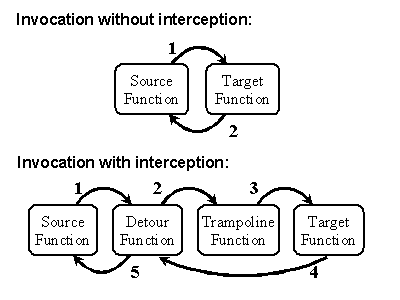
\includegraphics[width=\textwidth]{images/Detours_ovr_Technical_Figure_1.png}
		\caption{Detour/MinHook Execution Flow}
		\label{fig:Det}
	\end{subfigure}
	
	\vspace{1em} % Add some vertical space between the stacked images
	
	\begin{subfigure}{0.98\textwidth}
		\centering
		\includegraphics[width=\textwidth]{images/frida_flow.png}
		\caption{Frida-Gum Execution Flow}
		\label{fig:Frida}
	\end{subfigure}
	
	\caption{A comparison between the different architectures and roles of the Trampoline}
	\label{fig:instrumentation_comparison}
\end{figure}

\subsection{Instruction Boundaries and the Role of Disassemblers}

\note{Advisor}{cyan}{Non so se mettere questa sezione}
A fundamental challenge in implementing the hook structure described above, particularly on Intel x86 and x64 architectures, is the variable-length nature of the instruction set. To detour a target function, an inline hooking framework typically needs to overwrite the first few bytes of the function's prologue with an unconditional jump (\texttt{JMP}) to the custom payload. In a standard 32-bit architecture, this jump requires 5 bytes (1 byte for the opcode, 4 bytes for the relative address).

If the framework blindly overwrites exactly 5 bytes, it risks cutting an existing instruction in half. For example, if the original prologue consists of two 3-byte instructions, overwriting 5 bytes will corrupt the second instruction, leaving a hanging, invalid byte. When the trampoline attempts to execute these copied bytes to resume the program, the CPU will encounter an invalid opcode and crash the process.

To prevent this, hooking frameworks must incorporate a Length Disassembler Engine (LDE). Before applying any patches, the engine disassembles the target function's prologue to calculate exact instruction boundaries. It then copies whole, unfragmented instructions into the trampoline until it has safely relocated at least the number of bytes required for the jump (padding any remaining bytes in the original function with \texttt{NOP} instructions).

The choice of disassembler heavily impacts the footprint and dependencies of the framework:
\begin{itemize}
	\item \textbf{Microsoft Detours} relies on a proprietary, internal instruction decoder optimized specifically for standard compiler prologues.
	\item \textbf{MinHook} utilizes a highly optimized, custom-built Hacker Disassembler Engine (HDE32/HDE64), as it only needs to calculate instruction lengths rather than fully analyze instruction semantics.
	\item \textbf{Frida-Gum} requires deep semantic analysis of the instructions to achieve its context-aware routing. To accomplish this, it statically links against Capstone, a comprehensive and heavy multi-architecture disassembly framework, significantly increasing the size of the resulting \ac{DLL}.
\end{itemize}

\subsection{Transactional Patching: Safe Attachment and Detachment}

Another critical challenge in inline hooking is applying the memory patch (e.g., the \texttt{JMP} instruction) to a live, running process without causing a \textbf{race condition}. 
In a multi-threaded application, if one thread attempts to execute a target function at the exact moment the instrumentation framework is overwriting its prologue, the CPU may attempt to execute a partially written, invalid instruction.

To guarantee thread safety during the patching phase (both attaching and detaching), modern instrumentation frameworks implement a \textbf{transactional model}. Instead of patching memory directly and immediately, the developer queues the hooks. When the transaction is finalized, the framework briefly suspends all threads in the target process (except the one applying the patch), writes the bytes to memory atomically, flushes the CPU's Instruction Cache, and finally resumes the suspended threads.

\textbf{Detours} makes this transaction explicitly visible to the developer. The \ac{API} requires opening a transaction, manually declaring which threads need to be stopped, attaching/detaching the specified hooks, and committing the transaction:

\begin{lstlisting}[language=C++, caption={Microsoft Detours transactional model for safe attachment and detachment.}, label={lst:detours_lifecycle}, basicstyle=\ttfamily\footnotesize, breaklines=true]
		// --- SAFE ATTACHMENT ---
		// Start the transaction
		DetourTransactionBegin();
		
		// Enlist threads to be suspended during the patch
		DetourUpdateThread(GetCurrentThread()); 
		// here we specify possible other threads we want to stop...
		
		// Queue the hooks
		DetourAttach(&(PVOID&)TrueMessageBoxW, HookedMessageBoxW);
		// here we specify possible other hooks we want to inject...
		
		// Apply patches atomically, suspending the specified threads and flushing the instruction cache
		DetourTransactionCommit();
		
		
		// --- SAFE DETACHMENT ---
		DetourTransactionBegin();
		
		DetourUpdateThread(GetCurrentThread());
		// here we specify possible other threads we want to stop...
		
		DetourDetach(&(PVOID&)TrueMessageBoxW, HookedMessageBoxW); // Queue removal
		// here we specify possible other hooks we want to detach...
		
		DetourTransactionCommit();
		// Suspends threads, restores original bytes, resumes
	\end{lstlisting}

\textbf{MinHook} abstracts the explicit transaction start and end calls, but enforces the exact same synchronization internally when hooks are enabled or disabled (\Cref{lst:minhook_lifecycle}):

\begin{lstlisting}[language=C++, caption={MinHook internal thread synchronization during enable/disable phases.}, label={lst:minhook_lifecycle}, basicstyle=\ttfamily\footnotesize, breaklines=true]
		// --- SAFE ATTACHMENT ---
		MH_CreateHook(&MessageBoxW, &HookedMessageBoxW, reinterpret_cast<LPVOID*>(&fpMessageBoxW));
		// here we specify possible other hooks we want to inject...
		
		// MH_EnableHook internally suspends threads, writes the JMP, and resumes
		MH_EnableHook(&MessageBoxW);
		//or MH_EnableHook(MH_ALL_HOOKS); if we have more than one hook
		
		// --- SAFE DETACHMENT ---
		// MH_DisableHook internally suspends threads, restores original bytes, and resumes
		MH_DisableHook(&MessageBoxW);
		//or MH_DisableHook(MH_ALL_HOOKS); if we have more than one hook
	\end{lstlisting}

\textbf{Frida-Gum} employs an identical safety mechanism through its Interceptor \ac{API}:

\begin{lstlisting}[language=C, caption={Frida-Gum utilizing transaction boundaries for hook management.}, label={lst:frida_lifecycle}, basicstyle=\ttfamily\footnotesize, breaklines=true]
		// --- SAFE ATTACHMENT ---
		gum_interceptor_begin_transaction (interceptor);
		
		gum_interceptor_attach (interceptor,
		  GSIZE_TO_POINTER (gum_module_find_export_by_name (user32, "MessageBoxW")),
		  listener,
		  NULL,
		  GUM_ATTACH_FLAGS_NONE);
		// here we specify possible other hooks we want to inject...
		
		gum_interceptor_end_transaction (interceptor);
		// Threads are paused and patches applied
		
		// --- SAFE DETACHMENT ---
		gum_interceptor_begin_transaction (interceptor);
		
		gum_interceptor_detach (interceptor, listener);
		// here we specify possible other hooks we want to detach...
		
		gum_interceptor_end_transaction (interceptor);
		// Threads are paused and bytes restored
	\end{lstlisting}

\section{Dynamic Binary Instrumentation (\ac{DBI}) Architectures}

For deeper execution analysis at the assembly level, \ac{DBI} engines are utilized. Unlike inline hooking, which patches the original binary in place, \ac{DBI} engines ensure that the target application's original code is never executed directly by the CPU. Instead, the framework employs a \textbf{Just-In-Time (JIT) compilation} mechanism to dynamically translate and instrument instruction sequences.

\subsection{Core Architectural Components}
Modern \ac{DBI} frameworks rely on a unified architectural pattern comprising the following components:

\begin{description}
	\item[1. The Dispatcher (Control Flow Manager):] The dispatcher is the central component of the \ac{DBI} engine, responsible for orchestrating the execution state. Because the application and the \ac{DBI} framework share the same process but operate under different scopes, they must safely transit between ``framework mode" and ``application mode." The dispatcher trigger a context-switch mechanism that carefully saves and restores the application's state whenever execution exits or enters the code cache.
	\item[2. \ac{JIT} Compiler:] Instead of translating the entire binary before execution, these architectures translate the application's instructions dynamically in small fragments. During this translation phase, the framework decodes and encodes (into the framework's abstraction) the original instructions and has the opportunity to insert custom instrumentation code or patches before emitting the new sequence.
	\item[3. The Code Cache (The Execution Sandbox):] To mitigate the massive performance penalty of repeatedly translating the same code, \ac{DBI} frameworks employ a software-based code cache. The translated and potentially instrumented fragments are stored in this sandboxed memory region. When the application re-executes a previously translated section of code, it runs directly from the code cache, which significantly optimizes execution speed.
	\item[4. The Client Interface (Instrumentation API):] This is the abstraction layer exposed to the developer. It provides the necessary functions to inspect the program state, traverse instruction sequences, and specify exactly where and how instrumentation should be injected.
\end{description}

\subsection{The Execution Lifecycle: The JIT Loop}
To formally describe how these components interact at runtime, we can outline the execution lifecycle of a standard block of code:

\begin{enumerate}
	\item \textbf{Interception:} The target application attempts to execute a block of original code. The \ac{DBI} engine intercepts this attempt and yields control to the Dispatcher.
	\item \textbf{Cache Lookup:} The Dispatcher queries a fast-lookup hash table to check if the target memory address has already been translated. If it results in a cache hit, the CPU is redirected to the Code Cache.
	\item \textbf{Translation (On Cache Miss):} If the code has not been encountered before, the \ac{JIT} Compiler decodes original binary instructions one by one to form a straight-line sequence that terminates at a control transfer, such as a branch, call, or return.
	\item \textbf{Instrumentation:} The engine queries the Client Interface to determine if the user wishes to instrument the block or a single instruction within it. If so, the instrumentation instructions are injected. 
	\item \textbf{Emission and Linking:} Most \ac{DBI} frameworks use this phase to apply patches to the control-flow instructions at the end of the sequence, guaranteeing that when the block finishes running, it will redirect back to the framework rather than jumping to a native memory address. If the block ends in a direct branch to another previously translated block, the engine ``links'' them together directly in the cache (if it was an indirect branch, it cannot know the target before executing it), allowing the CPU to bypass the Dispatcher in future iterations. The modified block is emitted into the Code Cache.
	\item \textbf{Execution:} The Dispatcher performs a context switch, restoring the application state, and commands the CPU to execute the newly cached block natively.
	\item \textbf{Code Cache Exit:} Execution remains safely inside the code cache --- often jumping directly from one translated block to another through ``linking''---until it hits a boundary. This boundary might be an unlinked branch or an indirect branch whose target hasn't been translated yet. When this happens, the block executes an exit stub which saves the CPU's state and transfers control back to the Dispatcher, restarting the loop.
\end{enumerate}

\begin{figure}[H]
	\centering
	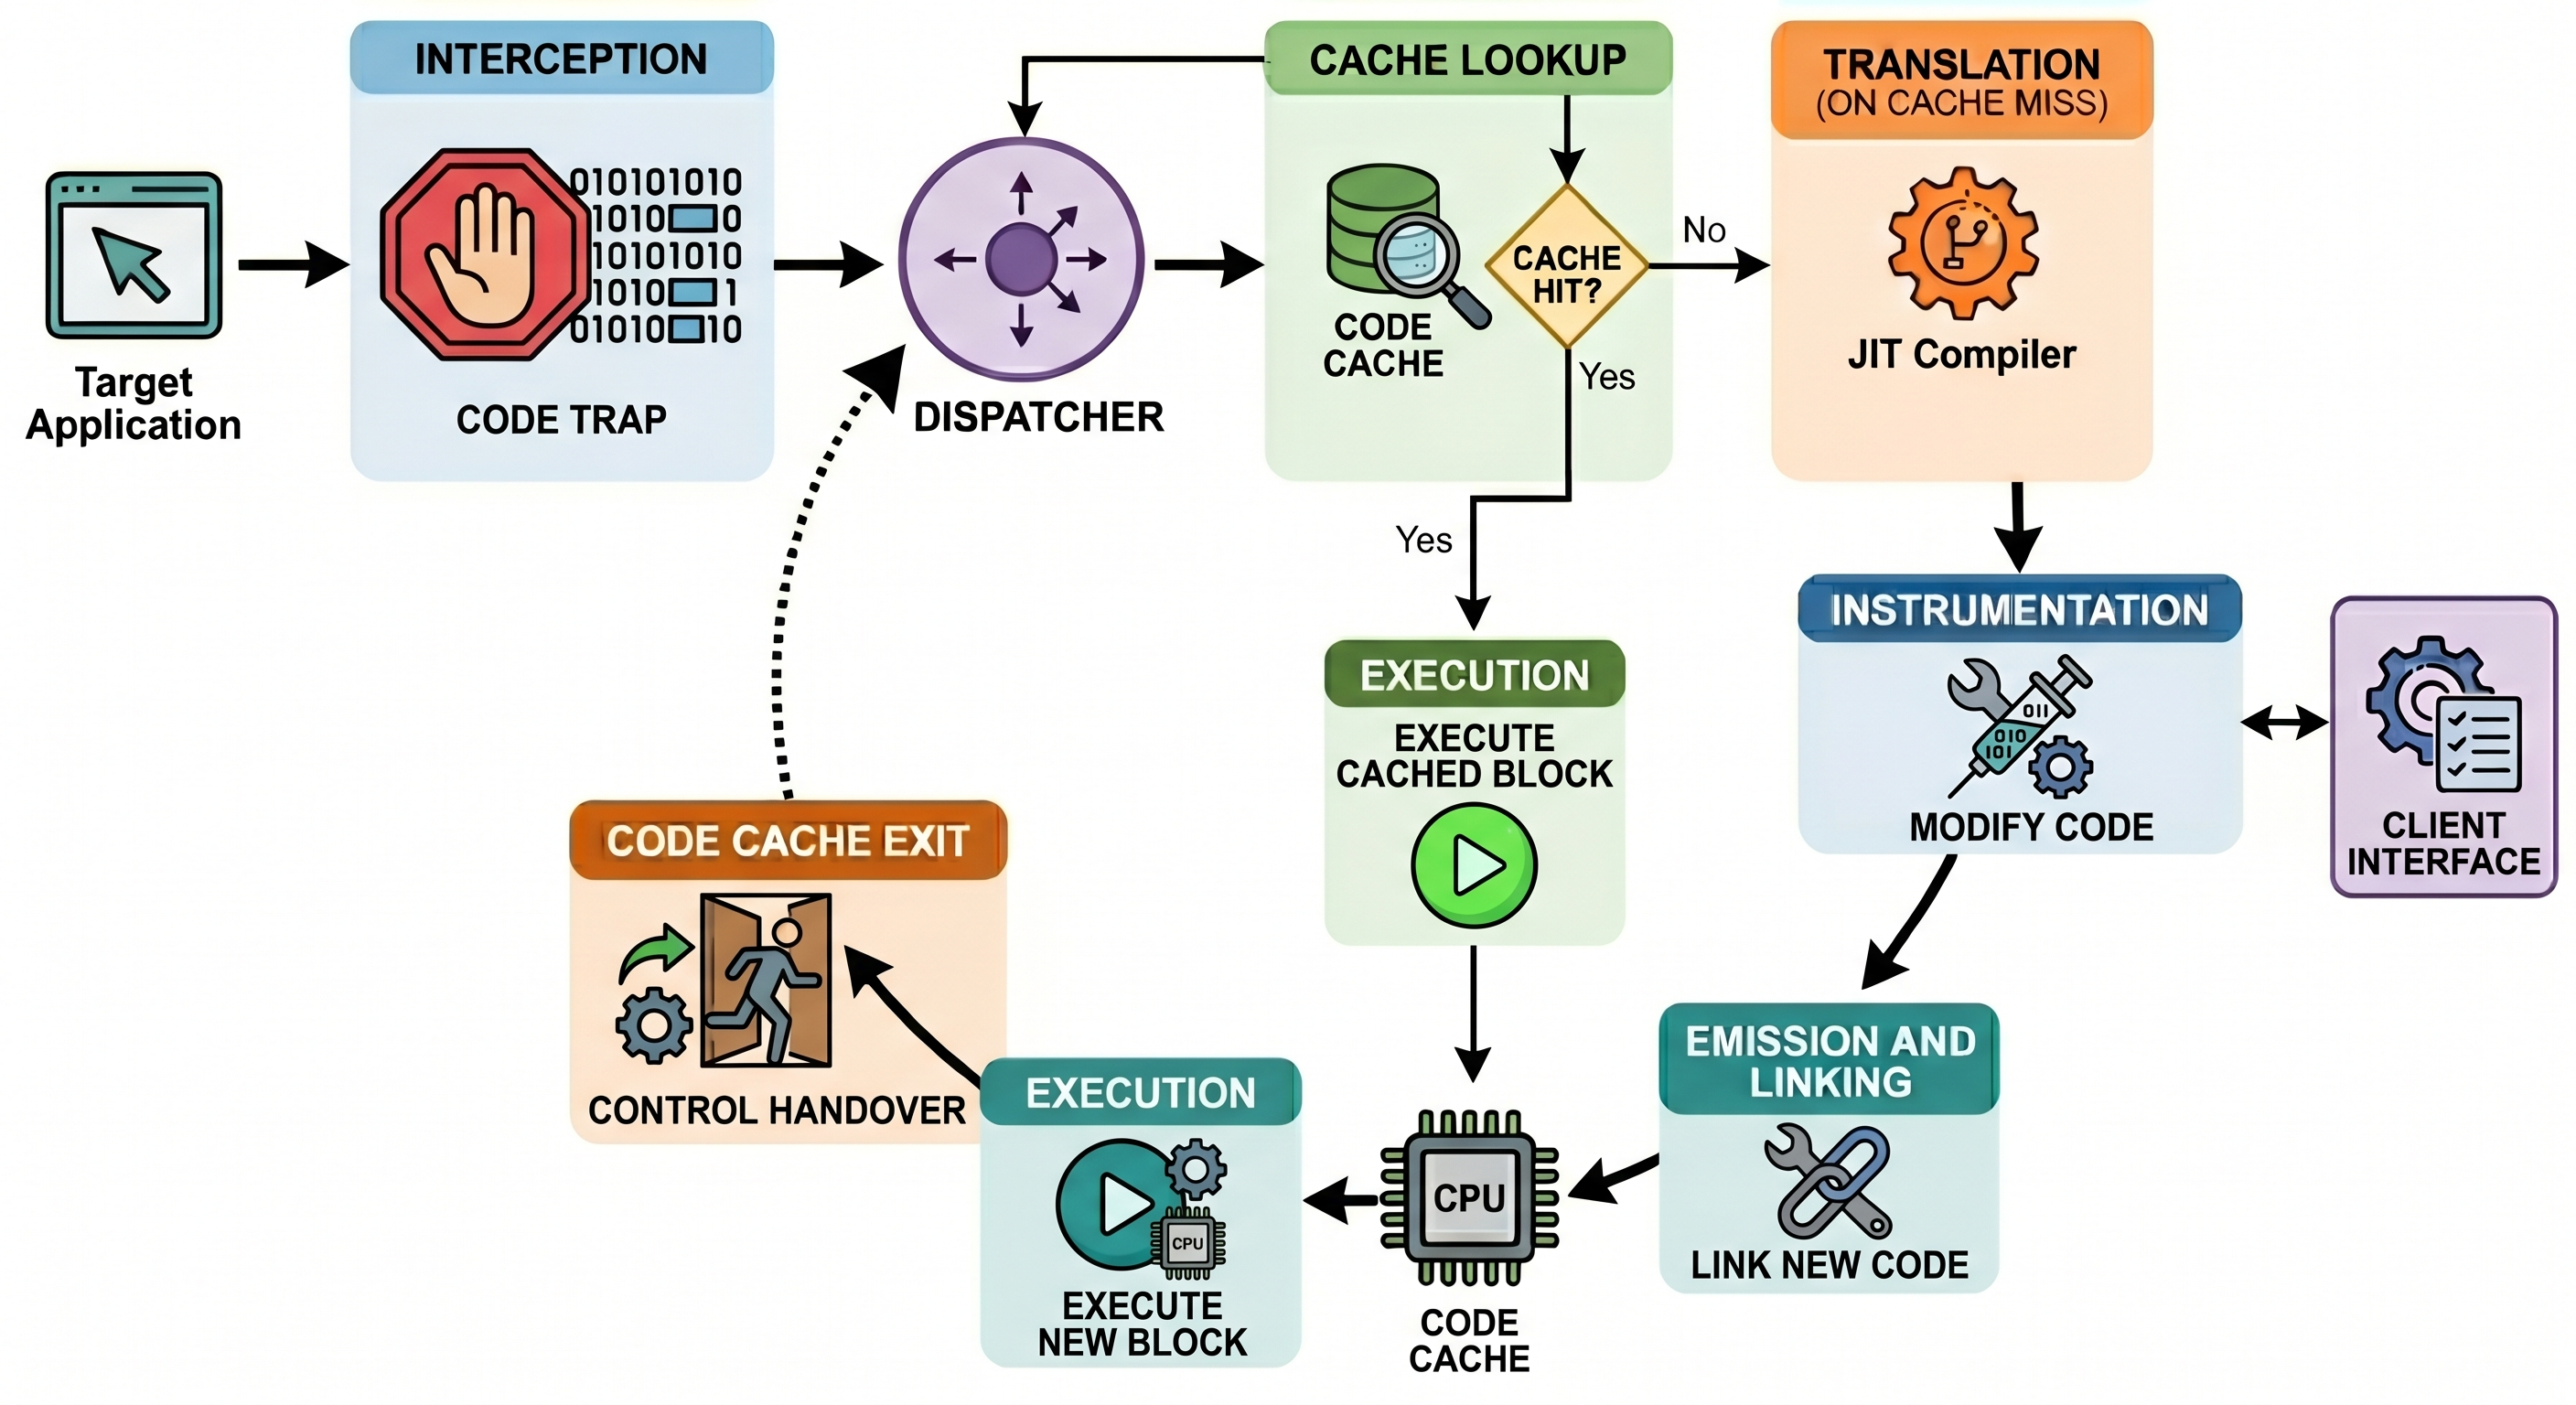
\includegraphics[width=0.9\textwidth]{images/DBI_flow.png}
	\caption{The Execution Lifecycle of a DBI framework}
	\label{fig:dbi_flow}
\end{figure}

While \ac{DBI} frameworks allow a more granular analysis of the target code, they introduce \textbf{significantly higher overhead} compared to inline hooking. Every single instruction of the program needs to be \ac{JIT}-compiled before execution, even if no instrumentation is injected.

\subsection{The Client Interface: Instrumentation vs. Analysis Functions}

\ac{DBI} frameworks require the developer to interact with the engine using a \textbf{two-tiered callback paradigm}. The developer must supply two distinct types of functions to the engine, each operating at fundamentally different times during the execution lifecycle:

\begin{itemize}
	\item \textbf{The Instrumentation Function (The ``Where'' and ``What''):} 
	This callback is invoked by the \ac{DBI} engine \emph{only once} per newly discovered sequence of instructions during the \ac{JIT} compilation phase. Its purpose is to inspect the static properties of the instructions (e.g., opcodes, operands) and decide \emph{if} and \emph{where} custom code should be injected. If injection is required, it uses the \ac{API} to queue the insertion of the analysis function.
	\item \textbf{The Analysis Function (The ``Action''):} 
	This is the actual custom payload injected into the Code Cache. Unlike the instrumentation function (executed only at compile time), it is executed \emph{every time} the CPU runs the corresponding instrumented block of code. For this reason, the analysis function must be heavily optimized and efficient.
\end{itemize}

The level of abstraction provided by the Client Interface significantly alters how developers interact with the engine.

\subsection{High-Level Abstraction: Intel PIN}
Intel PIN is a standard academic \ac{DBI} framework with a proprietary (free for non-commercial use) license. It provides a heavily abstracted C++ \ac{API}.

To utilize Intel PIN, developers do not modify the core engine itself. Instead, they write a custom C++ program known as a \emph{PINtool}. 
A PINtool represents the physical implementation of the Client Interface discussed previously; it is the user-defined module that contains both the Instrumentation Functions and the Analysis Functions. 

Architecturally, a PINtool is compiled as a standard shared library (a \ac{DLL} on Windows). When the user launches a target application under PIN, the engine automatically injects the PINtool \ac{DLL} into the target process's memory space. 
Once loaded, the engine invokes the PINtool's \texttt{main} function, allowing the tool to register its specific callbacks. 

In the following PINtool, we can observe the granularity achievable using \ac{DBI}: in this case, we can log conditional branches to determine which paths are taken during code execution.

\begin{lstlisting}[language=C++, caption={An example of a PINtool for branch logging}, label={lst:pin_branch}, basicstyle=\ttfamily\footnotesize, breaklines=true]
		// Analysis function (Runs at execution time in the Code Cache)
		void record_branch(ADDRINT instruction_address, ADDRINT target_address, BOOL taken) {
			
		  if (taken) { /* Log Taken */ } 
		  else       { /* Log Not Taken */ }
		}
		
		// Instrumentation function (Runs at JIT compilation time)
		void trace(INS instruction, void *v) {
			
		  // PIN abstracts away module resolution: we want to instrument
		  // only target application instructions, filter possible external libraries
		  RTN rtn = INS_Rtn(instruction);
		  
		  if (RTN_Valid(rtn) && IMG_IsMainExecutable(SEC_Img(RTN_Sec(rtn)))) {
		    // If it is inside the target executable, check if it's an IF branch
		    if (INS_IsBranch(instruction) && INS_HasFallThrough(instruction)) {
		      // Inject analysis function right before the jump happens.
		      INS_InsertCall(instruction, IPOINT_BEFORE, (AFUNPTR)record_branch,
		        IARG_INST_PTR,           
		        IARG_BRANCH_TARGET_ADDR,  
		        IARG_BRANCH_TAKEN,        
		        IARG_END);
		    }
		  }
		}
	\end{lstlisting}

\subsection{Bare-Metal \ac{DBI}: DynamoRIO}
DynamoRIO is the open-source alternative that exposes a lower-level C \ac{API}. 
The following code is the equivalent branch-logging example seen previously for PIN:

\begin{lstlisting}[language=C, caption={DynamoRIO branch instrumentation example}, label={lst:dr_branch}, basicstyle=\ttfamily\footnotesize, breaklines=true]
		// Analysis function
		static void record_branch(app_pc instr_addr, app_pc target_addr, int taken) {
		  
		  if (taken) { /* Log Taken */ } 
		  else       { /* Log Not Taken */ }
		}
		
		// Instrumentation function
		static dr_emit_flags_t event_bb_analysis(void *drcontext, void *tag, instrlist_t *bb, instr_t *inst, bool for_trace, bool translating,
		void *user_data) {
		  
		  // Manual module tracking to filter out OS libraries
		  app_pc instr_addr = instr_get_app_pc(inst);
		  
		  module_data_t *mod = dr_lookup_module(instr_addr);
		  bool is_main_exec = false;
		  
		  if (mod != NULL) {
		    module_data_t *main_mod = dr_get_main_module();
		    
		    if (main_mod != NULL) {
		      if (mod->start == main_mod->start) { is_main_exec = true; }
		      dr_free_module_data(main_mod);
		    }
		    dr_free_module_data(mod);
		  }
		  
		  if (!is_main_exec) return DR_EMIT_DEFAULT;
		  
		  // Check if it's a conditional branch (CBR)
		  if (instr_is_cbr(inst)) {
		    // Inject analysis function into the basic block (bb)
		    dr_insert_cbr_instrumentation(drcontext, bb, inst, (void *)record_branch);
		  }
		  return DR_EMIT_DEFAULT;
		}
	\end{lstlisting}

Using DynamoRIO, developers can directly manipulate the instruction flow. In PIN, developers generally ``wrap" existing instructions (adding a call before or after an instruction) but cannot easily modify the instruction itself. 
In DynamoRIO, the developer is handed a linked list of instructions (\texttt{instrlist\_t}) and can easily manipulate or modify them (e.g., reordering them or moving a load instruction earlier to test for race condition).

Furthermore, because PIN is designed to be highly opaque, using \texttt{INS\_InsertCall} prompts PIN's \ac{JIT} compiler to automatically analyze the custom analysis function for deciding which registers need to be saved and restored based on what the C++ code actually uses. 
With DynamoRIO, developers can manage the state and flags manually for specialized analysis.

In conclusion, while DynamoRIO may present a steeper learning curve than Intel PIN, it affords developers greater transparency and raw power, providing fine-grained control over the translated code and the code cache.

% \include{related}

\chapter{Methodology}
\label{ch:method}

This chapter presents the design, architecture, and implementation of HookDesigner: a declarative, multi-target transpilation and telemetry framework for Windows binary instrumentation.
The chapter is structured as follows:
\cref{sec:arch_overview} establishes the design principles, the overall architecture, and the target hooking engines.
\cref{sec:policy_dsl} introduces the declarative policy specification.
\cref{sec:code_gen} describes the template-driven code generation process.
\cref{sec:telemetry_engine} outlines the asynchronous logging and metrics collection subsystems.
\cref{sec:safety_fault_tolerance} examines runtime safety, crash prevention, and fault tolerance mechanisms.
Finally, \cref{sec:injection_lifecycle} details payload deployment, process injection, and safe module ejection.

\section{Design Principles and Architecture}
\label{sec:arch_overview}

The core objective of HookDesigner is to eliminate the gap between \emph{policy specification}---the \emph{what} of an instrumentation policy---and \emph{production-ready instrumentation code}---the \emph{how} of implementing that policy against a concrete hooking engine.
This gap is traditionally bridged by hand: a developer reads a policy document, then manually translates each requirement into engine-specific code.
However, handcrafting instrumentation code is notoriously error-prone due to the complete virtual address space sharing between the host application and the injected payload.
For this reason, subtle programming errors---such as dereferencing invalid parameters, or encountering race conditions in multi-threaded programs---inevitably result in unhandled crashes that terminate the entire host process.
Moreover, managing the lifecycle of hooks, including safe runtime attachment/detachment, produces fragile, tightly coupled to a specific engine code that is difficult to audit and maintain under changing requirements.

HookDesigner addresses this challenge through five foundational design principles.

\subsection{Design Principles}
\label{subsec:design_principles}

\begin{itemize}
	\item \textbf{Engine-Independent Transpilation}
	As analyzed in \fullref{sec:inline_hooking}, inline hooking engines expose different \acp{API}, and constraints on the instrumentation code.
	Rather than hard-coding engine details, HookDesigner treats each engine as a plug-in rendering target.
	A YAML engine registry (\texttt{engines.yaml}) maps engine names to Jinja2 template files, library paths, and linking arguments.
	The transpiler renders one complete C++ translation unit per engine in a single pass, producing compilable output.
	Adding a new engine requires only a new template and a registry entry; the core transpiler logic remains unchanged.
	
	\item \textbf{Crash Safety}
	As analyzed in \cref{subsec:address_space_isolation}, the instrumentation payload is mapped directly into the target application's private virtual address space.
	Consequently, any runtime error or unhandled memory access violation in the hook payload will crash the entire host process.
	HookDesigner enforces zero-crash safety through automated fault isolation, generating safe memory-access primitives around all parameter reads, pointer dereferences, and wrapping user callback executions and telemetry code in exception handlers.
	
	\item \textbf{Thread Safety}
	Hooking a running, multi-threaded process introduces synchronization issues during both hook installation/removal and module ejection (as analyzed in \cref{subsec:ejection_sync}).
	HookDesigner addresses these challenges through transactional patching models during attachment and detachment, combined with automatic thread-tracking guards embedded in each hook.
	
	\item \textbf{High-Performance Telemetry}
	To provide observability without damaging application responsiveness, the telemetry must introduce minimal overhead on critical execution paths.
	HookDesigner integrates industry-standard tools for high-performance telemetry, combining asynchronous logging via \texttt{spdlog} with lightweight metric exposition through \texttt{Prometheus}.
	This allows payloads to collect logs and real-time performance data with negligible latency impact on the host application.
	
	\item \textbf{Separation of Policy from Code}
	The instrumentation policy is expressed in a declarative YAML document that specifies \emph{which} functions are intercepted and \emph{what} behaviors are applied for each hook (logging rules, performance metrics, pre/post callbacks).
	The callback implementations and the target function signatures are authored separately in a standard C++ source file using a comment-based tagging convention, giving policy authors full IDE support and syntax highlighting.
	This separation allows also the same logic file to be reused across different policies and different target engines.
\end{itemize}

\subsection{The Seven-Stage Pipeline}
\label{subsec:pipeline}

HookDesigner processes an instrumentation request through a pipeline of seven stages.
The pipeline is split into two execution contexts: an \emph{offline} context executed on the developer's workstation (stages 1--4), and an \emph{online} context executed inside the target process' environment after the compiled \ac{DLL} has been transferred to the deployment machine (stages 5--7).

\begin{itemize}
	\item \textbf{Stage~1 -- Input:}
	The user provides two artifacts: a YAML policy file that declaratively specifies the instrumentation configuration, and a C++ logic file that contains the implementations of pre-hook and post-hook callbacks and the signature of the functions to instrument specified in the policy.
	The policy file declares the target process name, the logic file path, the selected engine(s), optional telemetry configuration, and the list of functions to hook with their associated behaviors.
	
	\item \textbf{Stage~2 -- Parse \& Validate:}
	The transpiler parses the YAML policy and validates its structural and semantic integrity against the schema, verifying consistency and cross-referencing declarations with data in the C++ logic file.
	
	\item \textbf{Stage~3 -- Generate:}
	The validated policy data are passed to the code generation engine. Using modular templates, the transpiler generatess complete, self-contained C++ source code tailored to the requested hooking engine.
	
	\item \textbf{Stage~4 -- Compile:}
	The generated C++ source files are compiled into Windows \acp{DLL}. The build process statically links the chosen instrumentation engine and telemetry backends, producing self-contained binaries without external runtime dependencies.
	
	\item \textbf{Stage~5 -- Inject:}
	The compiled \ac{DLL} is loaded into the target process by the injector utility (\texttt{injector.exe}, implemented in \texttt{injector.cpp}), which supports both attaching to an already-running process and launching a new process with the instrumentation payload active from its startup.
	
	\item \textbf{Stage~6 -- Execute:}
	Inside the running target, the injected hooks wrap target function, executing custom pre- and post-execution callbacks, recording performance metrics, and evaluating logging rules.
	
	\item \textbf{Stage~7 -- Eject:}
	When instrumentation terminates, the injector initiates a safe detachment procedure. Hook modifications are atomically reverted, and module unloading is coordinated with in-flight thread tracking to prevent process crashes.
\end{itemize}

A key consequence of the split into two execution contexts is that the online stages require no Python runtime, no \ac{LLVM}/LIBCLANG installation, and no access to the policy source---only the compiled \ac{DLL} and the injector binary are needed on the deployment host.
This is especially relevant for SCADA environments, where the target host is typically a resource-constrained, or sandboxed system that lacks developer runtimes and on which installing external dependencies or interpreters is usually blocked.

\subsection{HookDesigner Architecture}
\label{subsec:component_mapping}

To link the presented pipeline to the codebase, \cref{tab:component_mapping} maps each component of HookDesigner to its corresponding source files and responsibilities.

\begin{table}[H]
	\centering
	\small
	\begin{tabular}{p{3.2cm}p{4.0cm}p{6.6cm}}
		\toprule
		\textbf{Component} & \textbf{Source File} & \textbf{Responsibility} \\
		\midrule
		\textbf{Transpiler} & \texttt{transpiler.py} & Orchestrates parsing/validation, logic file validation, Jinja2 rendering, and MSVC compilation. \\
		\addlinespace
		\textbf{Engine Registry} & \texttt{engines.yaml} & Define engine specific templates, static libraries, and compiler flags. \\
		\addlinespace
		\textbf{Process Injector} & \texttt{injector.cpp} & Utility managing \ac{DLL} injection \& ejection. \\
		\addlinespace
		\textbf{Code Templates} & \texttt{templates/}
		\texttt{detours\_template.cpp} \newline
	 	\texttt{frida\_template.cpp}
		& Modular Jinja2 C++ templates generating engine-specific instrumentation code \\
		\bottomrule
	\end{tabular}
	\caption{Mapping of HookDesigner components to codebase files.}
	\label{tab:component_mapping}
\end{table}

\subsection{Selection of Compilation Targets}
\label{subsec:target_selection}

The architectural analysis and experimental results presented in \fullref{ch:background} directly guided the choice of instrumentation engines supported by HookDesigner.

For simplicity, I decided to start making HookDesigner compatible only with inline hooking paradigm (\cref{sec:inline_hooking}).

\begin{itemize}
	\item \textbf{Microsoft Detours:}
	Microsoft Detours was selected because, despite its minimalistic bare-metal model (analyzed in \cref{subsec:bare_metal_hooking}), it represents the gold standard for binary instrumentation in Windows x86 and x64 environments.
	By delegating execution routing directly to the detour function without intermediate layers (as illustrated in \cref{fig:Det}), Detours achieves near-zero runtime overhead, prioritizing execution speed over framework complexity. 
	
	\item \textbf{Frida-Gum:}
	Frida-Gum was chosen as a complementary engine to provide cross-architecture support and modern dynamic interception capabilities.
	However, as observed in \cref{subsec:scenario_2}, Frida-Gum's high-level \emph{Invocation Listener} mode introduces an \ac{ABI} limitation under the Windows x64 calling convention: its argument extraction \acp{API} index exclusively into General-Purpose Registers (\texttt{RCX}, \texttt{RDX}, \texttt{R8}, \texttt{R9}), failing to access floating-point parameters passed in vector registers (\texttt{XMM0}--\texttt{XMM3}).
	To bypass this constraint, HookDesigner targets only Frida-Gum's \emph{Function Replacement} mode (\texttt{gum\_interceptor\_replace} and \texttt{gum\_interceptor\_replace\_fast}, presented in \cref{subsec:frida_arch}).
	This allows developers to manually handle floating-point parameter extraction bypassing Frida indexing, while retaining some of Frida's built-in capabilities not included in Detours \ac{API}.
\end{itemize}

\section{Declarative Policy Specification and Logic File Integration}
\label{sec:policy_dsl}

This section analyzes the two input artifacts processed by HookDesigner in Stage~1 of its pipeline (\cref{subsec:pipeline}): the declarative YAML policy file, which defines \emph{what} functions to intercept and \emph{which} behaviors to attach, and the C++ user logic file, which implements \emph{how} pre/post callbacks behave.

\subsection{The Core YAML Policy DSL}
\label{subsec:yaml_policy_dsl}

The policy DSL is structured as a human-readable YAML document containing two top-level blocks: \texttt{configure}, which establishes global setting for the instrumentation, and \texttt{hooks}, which specifies the list of target functions to intercept along with their runtime address resolution strategies and optional code to inject (pre/post callbacks).

\subsubsection{The \texttt{configure} Block}

The \texttt{configure} section declares target process parameters, the relative path to the companion C++ logic file, the instrumentation paradigm and the correspondent target engines, as summarized in \cref{tab:configure_schema}.

\begin{table}[H]
	\centering
	\small
	\begin{tabular}{@{}llllp{6.0cm}@{}}
		\toprule
		\textbf{Field} & \textbf{Type} & \textbf{Req.} & \textbf{Default} & \textbf{Description} \\
		\midrule
		\texttt{process}      & string         & Yes & ---               & Target executable filename (e.g., \texttt{scada\_engine.exe}). \\
		\texttt{logic\_file}  & string         & Yes & ---               & Relative path (from the policy file) to the C++ logic source file. \\
		\texttt{engines}      & string / list  & No  & \texttt{"detours"} & Instrumentation engine(s) to generate code for. (e.g., \texttt{["detours", "frida"]}). \\
		\texttt{paradigm}     & string         & No  & \textit{inferred} & Hooking paradigm (e.g., \texttt{inline\_hook}). \\
		\texttt{telemetry}     & object         & No  & \texttt{\{\}} & Global Telemetry settings (detailed in \cref{sec:telemetry_engine}) \\
		\bottomrule
	\end{tabular}
	\caption{Schema definition for the top-level \texttt{configure} block.}
	\label{tab:configure_schema}
\end{table}

\begin{itemize}
	\item \texttt{engines} accepts either a single engine name or a list of target engines. When multiple engines are declared, the transpiler generates separate, engine-specific translation C++ files in a single invocation, enabling multi-engine deployments from a single policy definition.
	\item \texttt{paradigm} (for the moment can be only inline\_hook) explicitly declares the instrumentation paradigm. If specified, transpiler validates that all \texttt{engines} belong to this paradigm. If omitted, it is automatically inferred from the configuration registered in \texttt{engines.yaml} of the specified \texttt{configure.engines}.
\end{itemize}

\subsubsection{The \texttt{hooks} List}

The \texttt{hooks} section defines a sequence of hook configuration objects. Each entry specifies a target function to intercept, the runtime address resolution strategy to locate its address within \texttt{configure.process}, and the optional behavioral policies to apply, as detailed in \cref{tab:hook_schema}.

\begin{table}[H]
	\centering
	\small
	\begin{tabularx}{\textwidth}{@{}llcl>{\RaggedRight\arraybackslash}X@{}}
		\toprule
		\textbf{Field} & \textbf{Type} & \textbf{Req.} & \textbf{Default} & \textbf{Description} \\
		\midrule
		\texttt{function\_name}       & string       & Yes & ---                     & Target function name. \\
		\texttt{module}              & string       & No  & \texttt{""}             & Target \ac{DLL} module or \texttt{configure.process}. \\
		\texttt{is\_noreturn}        & bool         & No  & \texttt{false}          & Flag for non-returning functions. \\
		\texttt{address\_resolution} & object       & No  & \shortstack[l]{\texttt{\{strategy:}\\\texttt{~"export"\}}} & Strategy for runtime function address lookup. \\
		\texttt{behaviors}           & object       & No  & \texttt{\{\}}           & Sub-policies for metrics, logging, and callbacks. \\
		\midrule
		\multicolumn{5}{@{}l}{\textit{\textbf{Address Resolution Configuration (\texttt{address\_resolution})}}} \\
		\texttt{strategy}            & string       & Yes & ---                     & Resolution method: \texttt{"export"} or \texttt{"offset"}. \\
		\texttt{symbol\_name}        & string       & No  & \texttt{function\_name} & Exported decorated symbol for \texttt{GetProcAddress}. \\
		\texttt{rva\_offset}         & string / int & If offset & ---              & Hexadecimal \ac{RVA} offset (e.g., \texttt{"0x1A30"}). \\
		\midrule
		\multicolumn{5}{@{}l}{\textit{\textbf{Behavioral Sub-Policies Configuration (\texttt{behaviors})}}} \\
		\texttt{security\_policy}    & object       & No  & \texttt{\{\}}           & Custom pre-hook and post-hook callback bindings. \\
		\texttt{log\_rules}          & list         & No  & \texttt{[]}             &  Logging rules (detailed in \cref{sec:telemetry_engine}). \\
		\texttt{performance\_metrics}& object       & No  & \texttt{\{\}}           & Target latency and Prometheus metrics (detailed in \cref{sec:telemetry_engine}) \\
		\bottomrule
	\end{tabularx}
	\caption{Schema definition for the \texttt{hooks} list entries}
	\label{tab:hook_schema}
\end{table}

\begin{itemize}
	\item \textbf{Address Resolution Strategies:}
	\begin{itemize}
		\item \emph{Export Strategy (\texttt{strategy: export}):} Resolves the function entry address dynamically via \texttt{GetProcAddress}. When hooking C++ member functions or overloaded APIs where compiler name mangling alters the exported symbol name, the optional \texttt{symbol\_name} field allows specifying the decorated symbol.
		\item \emph{Offset Strategy} (\texttt{strategy:}\allowbreak\ \texttt{offset}): For unexported functions, HookDesigner computes its address at runtime by adding the specified hexadecimal \ac{RVA} offset (\texttt{rva\_offset}) to the base address of the specified \texttt{module}.
	\end{itemize}
	
	\item \textbf{Non-Returning Functions (\texttt{is\_noreturn}):} this flag is automatically inferred for standard non-returning \acp{API} (such as \texttt{RaiseException}, \texttt{ExitProcess}, and \texttt{ExitThread}). Because these functions never return to the caller, the transpiler leverages this flag either during semantic validation to prevent policy authors from defining post-trampoline callbacks or non-compatible telemetry features (\cref{subsec:static_semantic_validation}) and for correctly selecting the hook function structure designed for non-returning functions \cref{subsec:noreturn_adaptation}.
	\item \textbf{Security\_policy}: is a dictionary containing the user-defined \texttt{pre\_hook} name (executed prior to the trampoline) and \texttt{post\_hook} name (executed after original function completes) of the callbacks implemented in the C++ logic file.
\end{itemize}


\subsection{Logic File Integration}
\label{subsec:logic_file}

A core design principle of HookDesigner is the separation between declarative policy and imperative logic to inject, as presented in \cref{subsec:design_principles}.

For guiding the transpiler in parsing the logic file, it must present a specific structure built using tag markers:

\begin{enumerate}
	\item \textbf{Signatures Block} (\texttt{// @signatures-start} \dots\ \texttt{// @signatures-end}): 
	This block defines the exact parameter types, parameter order, optional calling conventions, and return types of the functions targeted by the policy.
	\item \textbf{Callback Implementation Regions} (\texttt{// @<CallbackName>-start}): 
	Each user callback implementation is prefixed with a dedicated tag matching the callback name referenced in the YAML policy's \texttt{security\_policy} dictionary (\texttt{pre\_hook} or \texttt{post\_hook}).
\end{enumerate}

The logic file will be included directly via \texttt{\#include} in the transpiler generated C++ file, so it can be used as a standard helper file.

\subsubsection{Clang Parsing}
\label{subsec:libclang_ast}

Parsing C++ function declarations using naive regular expressions is notoriously fragile due to complex types, pointer nesting, and calling conventions.
To guarantee correctness, Stage~2 of HookDesigner integrates CLANG via its Python bindings (\texttt{clang.cindex}).

The transpiler uses CLANG creates an in-memory Abstract Syntax Tree correspondent to the logic file with \texttt{-std=c++17} standard and traverses its nodes for performing the following task:

\begin{enumerate}
	\item \textbf{Extracting Signatures:} 
	The transpiler locates the Signatures Block and iterates over all function declarations. For every signatures node within this range, it extracts:
	\begin{itemize}
		\item The \emph{target function name} and \emph{return type}
		\item The \emph{calling convention} by scanning the token preceding the function identifier, looking for calling convention keywords (\texttt{\_\_stdcall}, \texttt{\_\_cdecl}, \texttt{\_\_fastcall}, etc.).
		\item The \emph{parameter list}, capturing parameter names and Clang type handles (\texttt{\_clang\_type}).
	\end{itemize}
	\item \textbf{Extracting Callback Parameters:}
	The transpiler scans for \texttt{// @<CallbackName>-}\allowbreak\texttt{start} tag patterns and filters the AST for matching \texttt{FUNCTION\_DECL} nodes, extracting parameter name for cross-validation against target function prototypes.
\end{enumerate}

During the parse and validation stage, the transpiler enforces the following semantic constraints:
\begin{itemize}
	\item \textbf{Signature Bindings:} Every \texttt{function\_name} specified in the YAML policy must have a corresponding function declaration inside the Signatures Block.
	\item \textbf{Callback Resolution:} Every callback identifier declared under \texttt{security\_policy} (\texttt{pre\_hook} - \texttt{post\_hook}) must have a matching \texttt{// @<CallbackName>-start} implementation in the logic file.
	\item \textbf{Parameter Matching:} Each callback parameter must match the name of a parameter in the target function's signature. Type checking and reference binding to the C++ compiler, since we could have arguments passed as reference or type aliases.
	\item \textbf{Return Value Overriding:} For \texttt{post\_hook} callbacks attached to non-void functions, an optional reference parameter matching the return type can be declared, enabling the callback to inspect or override the value returned to the caller.
\end{itemize}

\subsubsection{Callback Reusability}
\note{Advisor}{cyan}{Non so se mettere questa parte su Callback Reusability}

In some cases, sharing a pre/post callback across multiple distinct target functions could be useful for saving times and avoiding code duplication.
Because HookDesigner binds callback arguments by matching parameter names against the target function's parameters (delegating type checking and reference binding to the C++ compiler), developers can achieve callback reusability through parameter name alignment.

As illustrated in \cref{lst:reusability_example}, if two target routines (\texttt{UpdateSensorA} and \texttt{UpdateSensorB}) operate on a sensor reading under different parameter names, the developer unifies the parameter identifier to \texttt{val} in the \texttt{signatures} block. A single callback (\texttt{ChangeSensorValue}) can then be attached to both hooks in the YAML policy without duplicating logic.

\begin{lstlisting}[language=C++, caption={C++ user logic file illustrating callback reusability.}, label={lst:reusability_example}, basicstyle=\ttfamily\footnotesize, breaklines=true]
	
	// @signatures-start
	int UpdateSensorA(int sensorId, double val);
	int UpdateSensorB(double val, int flags);    
	// @signatures-end
	
	
	// @ChangeSensorValue-start
	void ChangeSensorValue(double& val) {
		if (val > 100.0) {
			val = 100.0;
		}
	}
\end{lstlisting}

To summarize the integration between declarative policy configuration and callback definitions, \cref{lst:policy_example} presents a complete YAML policy targeting multiple engines, combining export lookup, \ac{RVA} offset resolution, and injected user defined callbacks.

\begin{lstlisting}[language=SQL, caption={Example of core HookDesigner YAML policy}, label={lst:policy_example}, basicstyle=\ttfamily\footnotesize, breaklines=true]
	configure:
	paradigm: inline_hook
	engines:
	- detours
	- frida
	process: scada_engine.exe
	logic_file: "policy_logic.cpp"
	
	hooks:
	- function_name: QueuePut
	module: module.dll
	address_resolution:
	strategy: export
	security_policy:
	pre_hook: QueuePut_pre
	post_hook: QueuePut_post
	
	- function_name: UpdateSensor
	module: scada_engine.exe
	address_resolution:
	strategy: offset
	rva_offset: "0x1A30"
	security_policy:
	pre_hook: ChangeSensorValue
	
	- function_name: RaiseException
	is_noreturn: true
	address_resolution:
	strategy: export
\end{lstlisting}

The corresponding companion \texttt{logic\_file} (\texttt{policy\_logic.cpp}) is shown in \cref{lst:logic_example}. It illustrates the signature declarations block, tagged callback implementations with parameter mutation, and return value overriding.

\begin{lstlisting}[language=C++, caption={C++ logic file (\texttt{policy\_logic.cpp}) illustrating signature declarations, tag annotations, argument mutation by reference, and return value overrides.}, label={lst:logic_example}, basicstyle=\ttfamily\footnotesize, breaklines=true]
	#include <windows.h>
	#include <iostream>
	
	// @signatures-start
	int WINAPI QueuePut(void* pQueue, void* pEntry);
	int UpdateSensor(int sensorId, double val);
	void WINAPI RaiseException(DWORD dwExceptionCode, DWORD dwExceptionFlags, 
	DWORD nNumberOfArguments, const ULONG_PTR* lpArguments);
	// @signatures-end
	
	// @QueuePut_pre-start
	void QueuePut_pre(void*& pQueue, void*& pEntry) {
		if (pEntry == nullptr) {
			std::cout << "Blocked null entry in QueuePut\n";
		}
	}
	
	// @QueuePut_post-start
	void QueuePut_post(void* pQueue, void* pEntry, int& __hook_result) {
		if (__hook_result != 0) {
			std::cout << "[POST-LOGIC] Overriding failed QueuePut return code\n";
			__hook_result = 0;
		}
	}
	
	// @ChangeSensorValue-start
	void ChangeSensorValue(double& val) {
		if (val > 100.0) {
			val = 100.0;
		}
	}
\end{lstlisting}

After signature extraction and semantic validation, for each declared hook, the transpiler matches its \texttt{function\_name} against the extracted signatures, extending the hook's in-memory representation with its C++ return type, parameter list, and calling convention.
This merged data structure is subsequently passed to the Jinja2 template rendering engine in Stage~3 (\cref{sec:code_gen}).


\section{C++ Code Generation and DLL Compilation}
\label{sec:code_gen}

Once Stage~2 has validated the declarative policy and extracted the data within the logic file, Stage~3 and Stage~4 translate the in-memory policy representation into compilable C++ source code and build the final instrumentation DLL.
To realize the foundational principle of \emph{engine-independent transpilation} established in \cref{subsec:design_principles}, this phase must overcome a specific challenge: inline hooking engines expose fundamentally different low-level interfaces as examined in \fullref{sec:inline_hooking}.
Hard-coding engine-specific boilerplate into the transpiler would couple the transpilation process to specific frameworks, preventing the addition of new instrumentation engines without modifying the transpiler core.


To resolve this challenge, HookDesigner organizes code generation process through two different layers:
\begin{enumerate}
	\item An \textbf{external engine registry} (\texttt{engines.yaml}) that parameterises engine-specific template selection, cast expressions, and build arguments (\cref{subsec:engine_registry}).
	\item A \textbf{modular template hierarchy} that factors shared instrumentation logic into engine-independent partial templates while delegating specific features to engine templates (\cref{subsec:template_composition}).
\end{enumerate}

\subsection{Engine Registry}
\label{subsec:engine_registry}

The engine registry is a declarative YAML configuration file located at \texttt{engines.yaml} containing all engine-specific parameters.
The transpiler loads this file at startup via \texttt{load\_engines()} and uses it to drive all subsequent template rendering and compilation decisions.
With this registry, supporting a new hooking framework requires only providing an engine template and defining a registry entry; the Python parsing and validation remains unmodified.

\subsubsection{Registry Schema}

Engine entries are organized under a \emph{paradigm} top-level key that groups engines by their hooking model (e.g., \texttt{inline\_hook}).
This classification enables HookDesigner to support heterogeneous instrumentation paradigms (such as \ac{DBI} backends like DynamoRIO or Intel PIN, discussed in \cref{subsec:target_selection}).
\cref{tab:engine_registry_schema} documents the five required configuration fields mandated for every engine operating under the \texttt{inline\_hook} paradigm.

\begin{table}[H]
	\centering
	\small
	\begin{tabular}{@{}p{2.8cm}p{2.8cm}p{8.0cm}@{}}
		\toprule
		\textbf{Field} & \textbf{Type} & \textbf{Architectural Role} \\
		\midrule
		\texttt{template}      & string         & Filename of the engine's root Jinja2 template located in the \texttt{templates/} directory (e.g., \texttt{detours\_template.cpp}) \\
		\addlinespace
		\texttt{cast\_format}  & Python format string & Function-pointer cast expression. Captures engine-specific pointer typedef required. \\
		\addlinespace
		\texttt{libs\_arg}     & string         & Name of the CLI argument through which the static library path for the engine is passed to the transpiler. \\
		\addlinespace
		\texttt{inc\_arg}      & string         & Name of the CLI argument designating the engine's C/C++ header include directory \\
		\addlinespace
		\texttt{extra\_libs}   & list of strings & Additional Windows libraries statically linked into the generated \ac{DLL} \\
		\bottomrule
	\end{tabular}
	\caption{Schema definition for engine entries registered in \texttt{engines.yaml}.}
	\label{tab:engine_registry_schema}
\end{table}

\cref{lst:engines_yaml} lists the current registry configuration supporting Microsoft Detours and Frida-Gum.
The \texttt{cast\_format} field illustrates how the registry handles low-level engine differences without introducing conditional branching into the template files.
By encoding these conventions in \texttt{cast\_format}, the address resolution handler (\texttt{handle\_address\_resolution}, detailed in \cref{subsec:address_resolution}) emits the appropriate C++ cast expression directly in the transpilation process.

\begin{lstlisting}[language=SQL, caption={Current \texttt{engines.yaml} registry definition for Detours and Frida-Gum.}, label={lst:engines_yaml}, basicstyle=\ttfamily\footnotesize, breaklines=true]
	inline_hook:
	detours:
	template: "detours_template.cpp"
	cast_format: "(True{name}_t)"
	libs_arg: "detours_lib"
	inc_arg: "detours_include"
	extra_libs:
	- "User32.lib"
	- "Advapi32.lib"
	
	frida:
	template: "frida_template.cpp"
	cast_format: "(gpointer)"
	libs_arg: "frida_lib"
	inc_arg: "frida_include"
	extra_libs:
	- "User32.lib"
	- "Advapi32.lib"
	- "Ole32.lib"
	- "Shell32.lib"
\end{lstlisting}

\subsubsection{Registry Loading and Multi-Engine Validation}

The transpiler uses \texttt{load\_engines()} to parse \texttt{engines.yaml}, validating each entry against paradigm schemas: \texttt{inline\_hook} mandates all five fields in \cref{tab:engine_registry_schema}.
During policy validation (\texttt{validate\_policy}), the transpiler checks every declared engine (\texttt{configure.engines}) against the registry using \texttt{get\_engine\_config()} helper.
If a policy specifies multiple engines (e.g., \texttt{engines: ["detours", "frida"]}), the transpiler checks that all selected engines belong to the identical paradigm.

This check prevents incoherent code generation scenarios, such as simultaneously targeting two different paradigms from a single DSL policy.

\subsection{Jinja2 template architecture}
\label{subsec:template_composition}

HookDesigner generatess production-ready C++ instrumentation files through a modular Jinja2 template architecture.
A naive approach to multi-target code generation would maintain monolithic, duplicated template files for each supported engine.
However, with the framework we have selected, the majority of generated code is engine-independent.
Duplicating these code across engines would introduce maintenance issues.

\subsubsection{Two-Layer hierarchy}

To maximize code reuse while preserving engine autonomy, in HookDesigner templates are organized into a two-layer hierarchy:
\begin{enumerate}
	\item \textbf{Engine-Specific Templates} (\texttt{detours\_template.cpp}, \texttt{frida\_template.cpp}): 
	The files that define the translation skeleton. Each template defines module-level includes, global synchronisation primitives, function-pointer typedefs, and the exported \texttt{InitializeHooks} and \texttt{DeinitializeHooks} hooks lifecycle routines (\cref{subsec:lifecycle_functions}).
	\item \textbf{Shared Partial Templates} (\texttt{\_*.cpp}): Reusable partial templates located in \texttt{templates/}. Each file is included verbatim into the engine templates using the Jinja2 \texttt{\{\% include \%\}} directive.
\end{enumerate}

\cref{tab:partial_matrix} maps each partial template to its scope in the generated C++ code, its responsibility, and the section where its code is detailed.

\begin{table}[H]
	\centering
	\small
	\begin{tabularx}{\textwidth}{@{} l >{\RaggedRight}p{3.5cm} >{\RaggedRight}X >{\RaggedRight}p{2.3cm} @{}}
		\toprule
		\textbf{Partial File} & \textbf{Scope} & \textbf{Role} & \textbf{Reference} \\
		\midrule
		\texttt{\_telemetry\_globals.cpp} & Global scope, above functions & Declares global telemetry handles, metric family pointers, and metric label formatting utilities. & \cref{sec:telemetry_engine} \\
		\addlinespace
		\texttt{\_telemetry\_init.cpp}    & \texttt{InitializeHooks()} body & Initializes the logging subsystem and registers declared Prometheus metric families. & \cref{sec:telemetry_engine} \\
		\addlinespace
		\texttt{\_telemetry\_body.cpp}    & In-hook function (post trampoline invocation) & Evaluates declared logging rules and updates performance metric observations during hook execution. & \cref{sec:telemetry_engine} \\
		\addlinespace
		\texttt{\_user\_logic\_helpers.cpp} & Global scope, after headers & Provides runtime safety primitives: thread re-entrancy guards, active thread tracking, and safe memory access helpers. & \cref{sec:safety_fault_tolerance} \\
		\addlinespace
		\texttt{\_hook\_body.cpp}         & Inside each \texttt{Hooked<F>} function & Implements the required instrumentation payload for function F. & \cref{subsec:hook_function} \\
		\addlinespace
		\texttt{\_dllmain.cpp}            & end of generated file & Minimal DLL entry point & \cref{sec:injection_lifecycle} \\
		\bottomrule
	\end{tabularx}
	\caption{Template files and correspondent responsibility.}
	\label{tab:partial_matrix}
	\end{table}

Unlike the standard \ac{DLL} pattern presented in \cref{subsec:address_space_isolation} (where hook attachment and detachment are performed within \texttt{DllMain}), HookDesigner intentionally moves payload activation and ejection into standalone exported functions.
This separation is an architectural prerequisite to prevent Windows loader-lock deadlocks when installing complex hooks, as analyzed in \cref{subsec:lock_issue}.

Crucially, the bodies of \texttt{InitializeHooks} and \texttt{DeinitializeHooks} cannot be shared across engines: as established in \cref{subsec:transactional_patching}, guaranteeing thread safety during hook attachment and detachment requires engine-specific transactional models (such as Microsoft Detours' thread-enlisted prologue rewriting vs. Frida-Gum's dynamic interceptor runtime).

\subsubsection{Render Context}

Both engine-specific templates receive from the transpiler a \emph{render dictionary} consisting of three entries:
\begin{itemize}
	\item \texttt{hooks}: the list of hooks extracted in Stage~2, containing the hook policy data merged with the data derived from logic file (\cref{sec:policy_dsl}).
	\item \texttt{logic\_file\_rel}: The normalized relative filesystem path from the output C++ file to the companion user logic file (\cref{subsec:logic_file}), ensuring that the generated \texttt{\#include} directive resolves correctly across arbitrary build directories.
	\item \texttt{telemetry}: The telemetry configuration dictionary (or \texttt{None}), for managing the conditional rendering of logging and metrics C++ code (\cref{subsec:telemetry_dsl}).
\end{itemize}

\subsection{Target Address Resolution}
\label{subsec:address_resolution}

Before template rendering begins, the transpiler resolves the virtual address lookup expression for every declared hook and stores it in \texttt{hook["address\_resolution\_cpp"]}, this will be used by the hooks activation routine (\texttt{InitializeHooks()}, \cref{subsec:trans_attach_detach}).
To support both public exported \acp{API} and proprietary functions, HookDesigner provides two resolution strategies:
\begin{itemize}
	\item \textbf{Export Resolution:} For functions exposed in a module's Export Address Table (EAT), the transpiler generatess dynamic lookup via \texttt{GetProcAddress}, supporting custom or compiler-mangled symbol names where required.
	\item \textbf{Offset Resolution:} In proprietary software where internal subroutines are unexported, the transpiler generates \ac{RVA} pointer arithmetic relative to the module base (\texttt{GetModuleHandleA}), preserving address validity under ASLR.
\end{itemize}
To maintain engine independence, the resulting pointer expression is formatted according to the active engine's \texttt{cast\_format} (e.g., typed function pointers for Microsoft Detours vs. \texttt{gpointer} for Frida-Gum, as defined in \cref{tab:engine_registry_schema}), ensuring that templates remain decoupled from engine-specific type casting conventions.

\subsection{Hook Function Generation}
\label{subsec:hook_function}

For every function declared in the policy, HookDesigner generatess a replacement function named \texttt{Hooked<FunctionName>}.
As established in \cref{sec:abi}, to preserve stack alignment and register integrity across interception boundaries, the hooked function must match the target function's \ac{ABI} specifications exactly.
While 64-bit Windows environments unify calling conventions into a single paradigm, preserving calling convention qualifiers (e.g., \texttt{\_\_stdcall}, \texttt{\_\_cdecl}) remains critical for multi-architecture portability and 32-bit targets.

The transpiler achieves strict fidelity by rendering the function signature directly from the metadata extracted from the logic file in Stage~2 (\cref{subsec:libclang_ast}), as illustrated in the template definition in \cref{lst:function_signature}:
\begin{lstlisting}[language=C++, caption={Hook function signature rendering template.}, label={lst:function_signature}, basicstyle=\ttfamily\footnotesize, breaklines=true]
	{{ hook.return_type }} {% if hook.calling_convention %}{{ hook.calling_convention }} {% endif %}Hooked{{ hook.function_name }}({%- for param in hook.parameters -%}{{ param.type }} {{ param.name }}{%- if not loop.last -%}, {%- endif -%}{%- endfor -%})
\end{lstlisting}

While the classic inline hook function structure (\cref{sec:inline_hooking}) follows a basic three-step pattern (\emph{pre-logic} $\rightarrow$ \emph{trampoline dispatch} $\rightarrow$ \emph{post-logic}), deploying such a function into a live, multi-threaded process could be dangerous: an unhandled exception inside an injected callback crashes the host application, recursive API calls cause stack overflow, in-flight threads crash during DLL unloading.

For this reason in HookDesigner, the body of each hooked function (\texttt{\_hook\_body.cpp}) extend this basic pattern with automated telemetry collection (\cref{sec:telemetry_engine}), and runtime safety defenses (\cref{sec:safety_fault_tolerance}).
The complete, production in-hook execution structure is showed in detail in \cref{subsec:hook_pipeline}.


\subsection{Hook Lifecycle Function Generation}
\label{subsec:lifecycle_functions}

In addition to individual hook functions (\cref{subsec:hook_function}), the generated code must provide entrypoints responsible for orchestrating the overall lifecycle of the instrumentation DLL.
HookDesigner generate two exported functions with standard C linkage: \texttt{InitializeHooks()}, which resolves targets and installs the hooks upon injection, and \texttt{DeinitializeHooks()}, which detaches them prior to unloading.

\subsubsection{Transactional Attachment and Detachment}
\label{subsec:trans_attach_detach}

Once the target functions are located, the template performs batch hook registration using the engine's transactional API, building on the transactional patching principles established in \cref{subsec:transactional_patching}.
Transactional execution guarantees atomicity: either all valid hooks are committed simultaneously, or the entire transaction fails without leaving the process in a partially patched, unstable state.

Symmetrically, during payload deinitialization, an atomic detachment transaction reverts the patches and restores the original instructions.

Depending on the active hooking engine, the template emits the corresponding transactional loops across the declared hooks, as illustrated in \cref{lst:detours_lifecycle_template} for Microsoft Detours and \cref{lst:frida_lifecycle_template} for Frida-Gum.

\begin{lstlisting}[language=C++, caption={Simplified Jinja2 template logic for Microsoft Detours hook lifecycle functions.}, label={lst:detours_lifecycle_template}, basicstyle=\ttfamily\footnotesize, breaklines=true]

extern "C" __declspec(dllexport) void InitializeHooks() {
    // 1. Locate Functions
    {% for hook in hooks %}
    	True{{ hook.function_name }} = {{ hook.address_resolution_cpp }};
    {% endfor %}

    // 2. Transactional Attachment
    DetourTransactionBegin();
    DetourUpdateThread(GetCurrentThread());
    {% for hook in hooks %}
    if (True{{ hook.function_name }}) {
        DetourAttach(&(PVOID&)True{{ hook.function_name }}, (PVOID)Hooked{{ hook.function_name }});
    }
    {% endfor %}
    DetourTransactionCommit();
}

extern "C" __declspec(dllexport) BOOL DeinitializeHooks() {
    // Transactional Detachment / Reversion
    DetourTransactionBegin();
    DetourUpdateThread(GetCurrentThread());
    {% for hook in hooks %}
    if (True{{ hook.function_name }}) {
        DetourDetach(&(PVOID&)True{{ hook.function_name }}, (PVOID)Hooked{{ hook.function_name }});
    }
    {% endfor %}
    DetourTransactionCommit();
    
}
\end{lstlisting}

\begin{lstlisting}[language=C++, caption={Simplified Jinja2 template logic for Frida-Gum hook lifecycle functions.}, label={lst:frida_lifecycle_template}, basicstyle=\ttfamily\footnotesize, breaklines=true]

extern "C" __declspec(dllexport) void InitializeHooks() {
    gum_init_embedded();
    interceptor = gum_interceptor_obtain();

    // 1. Locate Functions
    {% for hook in hooks %}
    	True{{ hook.function_name }} = {{ hook.address_resolution_cpp }};
    {% endfor %}

    // 2. Transactional Replacement
    gum_interceptor_begin_transaction(interceptor);
    {% for hook in hooks %}
    if (target_{{ hook.function_name }}) {
        gum_interceptor_replace(interceptor,
                                target_{{ hook.function_name }},
                                (gpointer)Hooked{{ hook.function_name }},
                                nullptr,
                                (gpointer*)&True{{ hook.function_name }});
    }
    {% endfor %}
    gum_interceptor_end_transaction(interceptor);
}

extern "C" __declspec(dllexport) BOOL DeinitializeHooks() {
    // Transactional Reversion
    gum_interceptor_begin_transaction(interceptor);
    {% for hook in hooks %}
    if (target_{{ hook.function_name }} != nullptr) {
        gum_interceptor_revert(interceptor, target_{{ hook.function_name }});
    }
    {% endfor %}
    gum_interceptor_end_transaction(interceptor);

    return TRUE;
}
\end{lstlisting}

While \cref{lst:detours_lifecycle_template,lst:frida_lifecycle_template} illustrate the simplified Jinja2 template loops used to generate batch attachment and detachment, deploying these routines into a live, multi-threaded process requires additional safeguards to coordinate thread synchronization, handle telemetry subsystems, and prevent loader-lock deadlocks.
The complete runtime execution sequence of \texttt{InitializeHooks()} and \texttt{DeinitializeHooks()} is detailed in \cref{sec:injection_lifecycle}.



\subsection{DLL Compilation}
\label{subsec:compilation}

The generated C++ is compiled into a 64-bit (or 32-bit) Windows \ac{DLL} by \texttt{compile\_dll()}.
The transpiler locates the MSVC compiler by invoking Microsoft's \texttt{vcvars64.bat} environment script through a spawned subprocess, eliminating the requirement for manual  configuration.
To assemble the complete build command, \texttt{compile\_dll()} combines the compiler flags in \cref{tab:compiler_flags} with the engine-specific settings retrieved from \texttt{engines.yaml} (\cref{subsec:engine_registry}).

\cref{tab:compiler_flags} documents the specific compiler flags applied to \texttt{cl.exe} and their justifications.

\begin{table}[H]
	\centering
	\small
	\begin{tabular}{@{}llp{8.5cm}@{}}
		\toprule
		\textbf{Flag} & \textbf{Category} & \textbf{Behavior} \\
		\midrule
		\texttt{/LD}       & Linker Mode      & Instructs MSVC to produce a Dynamic-Link Library (\ac{DLL}) \\
		\addlinespace
		\texttt{/EHa}      & Exception Model  & Enables asynchronous \ac{SEH} translation. (\cref{subsec:seh}). \\
		\addlinespace
		\texttt{/O2}       & Optimization     & Minimizes Interception Overhead on APIs called at high frequencies \\
		\addlinespace
		\texttt{/utf-8}    & Source Encoding  & Enforces UTF-8 character encoding across source files, ensuring cross-platform consistency. \\
		\addlinespace
		\texttt{/std:c++17}& Language Standard& Enables C++17 language constructs\\
		\addlinespace
		\texttt{/MT}       & CRT Linkage      & Statically links the C Runtime Library (\texttt{libcmt.lib}), completely eliminating external runtime dependencies on \texttt{msvcp140.dll}. \\
		\bottomrule
	\end{tabular}
	\caption{MSVC compiler flags utilized in \texttt{compile\_dll()} and their behavior}
	\label{tab:compiler_flags}
\end{table}

\paragraph{DLL portability}
A key design constraint for HookDesigner is operational reliability in restricted industrial \ac{SCADA} settings.

If the instrumentation \ac{DLL} were dynamically linked against the universal CRT (\texttt{/MD}), loading the payload onto a target machine lacking the exact corresponding redistributable build would trigger a loader failure, silently failing injection.
By enforcing static CRT linkage (\texttt{/MT}) and statically linking the hooking engine (Detours or Frida-Gum) alongside the telemetry libraries (\texttt{spdlog} and \texttt{prometheus-cpp}), the transpiler outputs a completely self-contained binary.
The resulting \ac{DLL} carries zero dependencies beyond core Windows system libraries, guaranteeing reliable injection into restricted industrial environments.


\section{Telemetry in HookDesigner}
\label{sec:telemetry_engine}

In industrial SCADA environment, critical functions frequently execute thousands of times per second across concurrent worker threads.
When instrumenting such processes, where performances are essential, telemetry cannot come at the expense of host responsiveness.
A naive instrumentation strategy that performs heavy tasks (such as executing blocking disk writes, or querying network endpoints directly within the hook function) introduces latency spikes and thread contention, destabilizing the monitored system.

To overcome these constraints and fulfill the \emph{High-Performance Telemetry} design principle introduced in \cref{subsec:design_principles}, HookDesigner implements the following solutions:
\begin{enumerate}
	\item \textbf{Asynchronous Logging (\cref{subsec:async_logging}):} A non-blocking logging mechanism powered by \texttt{spdlog}, utilizing a pre-allocated bounded ring buffer that decouples hot-path hook execution from background I/O draining.
	\item \textbf{Real-Time Performance Metrics (\cref{subsec:prometheus}):} A native Prometheus metrics subsystem based on \texttt{prometheus-cpp}, exposed through an embedded HTTP server.
\end{enumerate}

Before generating code, the framework processes telemetry policy rules during transpilation: \cref{subsec:telemetry_dsl} defines the declarative YAML schema and static validation constraints.

\subsection{Telemetry Policy Specification}
\label{subsec:telemetry_dsl}

HookDesigner defines telemetry behaviors declaratively within the policy document introduced in \cref{subsec:yaml_policy_dsl}.
Telemetry configuration is split into two distinct components: process-wide parameters declared in the top-level \texttt{configure.telemetry} block, and hook-specific behavioral policies declared under each hook entry's \texttt{behaviors} mapping.

\subsubsection{Global Telemetry Configuration}

The top-level \texttt{configure.telemetry} mapping establishes the general settings for the logging framework and the metric server endpoint.
\cref{tab:telemetry_configure_schema} outlines the schema definitions for this block.

\begin{table}[H]
	\centering
	\small
	\begin{tabularx}{\textwidth}{@{} l l l l X @{}}
		\toprule
		\textbf{Field} & \textbf{Type} & \textbf{Req.} & \textbf{Default} & \textbf{Description} \\
		\midrule
		\texttt{logger}        & string & No  & \texttt{null} & Logging engine identifier (currently supports \texttt{"spdlog"}). \\
		\texttt{logger\_config} & object & No  & \texttt{\{\}} & if \texttt{logger} not \texttt{null}, log configuration \\
		\texttt{metrics}       & string & No  & \texttt{null} & Metrics engine identifier (currently supports \texttt{"prometheus"}). \\
		\texttt{metrics\_config}& object & No  & \texttt{\{\}} & if \texttt{metrics} not \texttt{null}, HTTP exposer configuration. \\
		\midrule
		\multicolumn{5}{@{}l}{\textit{\textbf{Logger Settings (\texttt{logger\_config})}}} \\
		\texttt{type}          & string & No  & \texttt{"file"} & Log destination: \texttt{"file"} (local disk) or \texttt{"udp"} (remote Syslog). \\
		\texttt{host}          & string & No  & \texttt{"127.0.0.1"} & Target host IPv4 address only if \texttt{type: "udp"}. \\
		\texttt{port}          & integer& No  & \texttt{1514} & Target \ac{UDP} listening port only if \texttt{type: "udp"}. \\
		\texttt{file}          & string & No  & \texttt{"hook\_log.txt"} & Destination file path only if \texttt{type: "file"}. \\
		\texttt{level}         & string & No  & \texttt{"info"} & Minimum severity filter (\texttt{trace}, \texttt{debug}, \texttt{info}, \texttt{warn}, \texttt{error}, \texttt{critical}). \\
		\midrule
		\multicolumn{5}{@{}l}{\textit{\textbf{Metrics Exposer Endpoint (\texttt{metrics\_config})}}} \\
		\texttt{endpoint}      & string & No  & \texttt{"127.0.0.1:8080"} & Address and port bound by the embedded Prometheus HTTP server. \\
		\bottomrule
	\end{tabularx}
	\caption{Schema definition for the top-level \texttt{configure.telemetry} block.}
	\label{tab:telemetry_configure_schema}
\end{table}

\subsubsection{Hook-Level Telemetry Behaviors}

At the granularity of individual hooks, the \texttt{behaviors.performance\_metrics/log\_rules} defines logging and performance metrics rules to inject in the \texttt{hook.target\_function}.
Hook-level telemetry is configured across two sub-mappings:
\begin{itemize}
	\item \texttt{log\_rules}: A list of conditional rule objects specifying log severity, triggering conditions, and emitted message formats.
	\item \texttt{performance\_metrics}: flag for execution latency tracking and Prometheus canonical metrics configuration.
\end{itemize}

Within the metrics configuration, an optional \texttt{label} key-value mapping can be declared.
In Prometheus, labels (\cref{subsubsec:metric_labels}) allow a single metric family to partition its observations dynamically according to runtime execution context (e.g., classifying a function invocation counter by return status or error code).

\cref{tab:telemetry_behaviors_schema} documents the schema for these behavioral sub-policies.

\begin{table}[H]
	\centering
	\small
	\begin{tabularx}{\textwidth}{@{} l l l l X @{}}
		\toprule
		\textbf{Field} & \textbf{Type} & \textbf{Req.} & \textbf{Default} & \textbf{Description} \\
		\midrule
		\multicolumn{5}{@{}l}{\textit{\textbf{Performance Metrics Policy (\texttt{behaviors.performance\_metrics})}}} \\
		\texttt{execution\_time} & bool & No & \texttt{false} & Enables \texttt{target\_function} latency measurement\\
		\texttt{counters}        & list & No & \texttt{[]}    & Counter metric definitions \\
		\texttt{gauges}          & list & No & \texttt{[]}    & Gauge metric definitions \\
		\texttt{histograms}      & list & No & \texttt{[]}    & Histogram metric definitions \\
		\midrule
		\multicolumn{5}{@{}l}{\textit{\textbf{Metric Instrument Schema (Counters, Gauges, Histograms)}}} \\
		\texttt{name}            & string & Yes & --- & Unique metric identifier within the hook function. \\
		\texttt{description}     & string & No  & \texttt{""} & Human-readable help string exported to the Prometheus registry. \\
		\texttt{condition}       & string & No  & \texttt{"true"} & Boolean expression indicating when the observation occurs. \\
		\texttt{value}           & string & Gauges/Hists & --- & C++ numerical expression to record (e.g., \texttt{latency}, parameter). \\
		\texttt{buckets}         & list   & No (Hists) & \textit{default} & Custom strictly increasing positive bucket upper bounds only for histograms. \\
		\texttt{label}           & dict   & No  & \texttt{\{\}} & Dynamic key-value label mapping for dimensional partitioning. \\
		\midrule
		\multicolumn{5}{@{}l}{\textit{\textbf{Logging Rule Schema (\texttt{behaviors.log\_rules})}}} \\
		\texttt{name}            & string & No  & \texttt{"rule\_N"} & Unique rule name identifier within the hook \\
		\texttt{level}           & string & No  & \texttt{"info"} & Log severity level (\texttt{trace}, \texttt{debug}, \texttt{info}, \texttt{warn}, \texttt{error}, \texttt{critical}). \\
		\texttt{condition}       & string & No  & \texttt{"true"} & Boolean expression evaluated at runtime to trigger logging. \\
		\texttt{arguments}       & list   & No  & \texttt{[]}    & Parameter identifiers captured for auto-generated format strings. \\
		\texttt{format}          & string & No  & \texttt{null}  & Custom message format string supporting positional format specifierws. \\
		\bottomrule
	\end{tabularx}
	\caption{Schema definition for hook-level logs and metrics}
	\label{tab:telemetry_behaviors_schema}
\end{table}

\subsubsection{Logging Rule Declaration Modalities}
\label{subsubsec:log_rule_modalities}

In binary instrumentation, logging formats can vary widely across different inspection environments.
During exploratory reverse engineering, an analyst often requires rapid, call-graph tracing log to understand execution control flow.
Conversely, during an incident response, logs should be able to capture precise parameter states and outcome codes formatted to match external ingestion tools.

To reconcile these different requirements, HookDesigner supports different declaration modalities within \texttt{behaviors.log\_rules}, illustrated in \cref{lst:log_rule_modalities}:
\begin{enumerate}
	\item \textbf{Default / Empty Rule (\texttt{-\ \{\}}):} Injects a function invocation log using default metadata (\texttt{name: "rule\_1"}, \texttt{level: "info"}, \texttt{condition: "true"}), only for checking if the target\_function is called.
	\item \textbf{Default Rule with Arguments:} The policy author can specify target function parameters to include in the log; the transpiler validates argument identifiers against the target signature and generates a structured, pipe-delimited key-value format string automatically.
	\item \textbf{Custom Format String:} Parses tokens matching \texttt{\{placeholder\}} (supporting format specifiers like \texttt{:x} or \texttt{:.2f}) and emits a pre-compiled positional \texttt{fmtlib} template representing the custom log.
	\item \textbf{Multi-Rule:} Emits independent sequential C++ \texttt{if} blocks for generating logs evaluated against return codes or runtime arguments.
	\item \textbf{No Logging (\texttt{log\_rules:\ []}):} Completely eliminates all logging code generation
\end{enumerate}


\begin{lstlisting}[language=SQL, caption={Demonstration of the logging rule declaration modalities}, label={lst:log_rule_modalities}, basicstyle=\ttfamily\footnotesize, breaklines=true]
hooks:
  # Modality 1: Empty Rule
  - function_name: CreateFileW
    module: "kernel32.dll"
    behaviors:
      log_rules:
        - {}  # Emits: "[HOOK CreateFileW] [rule_1] called"

  # Modality 2: Default Rule with Arguments
  - function_name: UpdatePacket
    module: "user32.dll"
    behaviors:
      log_rules:
        - name: "dpi_trace"
          level: "debug"
          arguments:
            - input_hWnd
            - input_dwFlags
          # Emits: "[HOOK SetProcessDPIAware] [dpi_trace] | input_hWnd={hWnd} | input_dwFlags={flags}"

  # Modality 3: Custom format string with format specifiers (:x)
  - function_name: RegOpenKeyExA
    module: "advapi32.dll"
    behaviors:
      log_rules:
        - name: "reg_failure"
          condition: "__hook_result != 0"
          level: "warn"
          format: "[WARN] RegOpenKeyExA FAILED | key={input_lpSubKey} access=0x{input_samDesired:x} err={__hook_result}"
          # Emits: "[WARN] RegOpenKeyExA FAILED | key=12 access=0x20019 err=2"

  # Modality 4: Multi-rule
  - function_name: DispatchPacket
    module: "scada_engine.exe"
    behaviors:
      log_rules:
        - name: "on_success"
          condition: "__hook_result == 0"
          level: "debug"
          arguments:
            - input_packetId
          # Emits on success: "[HOOK DispatchPacket] [on_success] | input_packetId=13"
        - name: "on_failure"
          condition: "__hook_result != 0"
          level: "error"
          format: "[ERROR] Dispatch failed | id={input_packetId} code={__hook_result} latency={latency:.2f}ms"
          # Emits on failure: "[ERROR] Dispatch failed | id=101 code=-1 latency=12.45ms"

  # Modality 5: No logging
  - function_name: HighFrequencyTimerTick
    module: "scada_engine.exe"
    behaviors:
      log_rules: []  # Emits: nothing
\end{lstlisting}

\cref{lst:telemetry_policy_snippet} provides a YAML policy snippet demonstrating the integration of latency tracking, Prometheus counters and histograms with dynamic labels, and multi-condition log routing.

\begin{lstlisting}[language=SQL, caption={Example YAML with telemetry configuration}, label={lst:telemetry_policy_snippet}, basicstyle=\ttfamily\footnotesize, breaklines=true]
configure:
  process: "scada_engine.exe"
  logic_file: "scada_logic.cpp"
  telemetry:
    logger: "spdlog"
    logger_config:
      type: "udp"
      host: {ip_addr}
      port: 1514
      level: "info"
    metrics: "prometheus"
    metrics_config:
      endpoint: "0.0.0.0:8085"

hooks:
  - function_name: ParseProprietaryPacket
    module: "scada_engine.exe"
    address_resolution:
      strategy: export
    behaviors:
      performance_metrics:
        execution_time: true
        counters:
          - name: "packets_total"
            description: "Total proprietary packets processed"
            label:
              status: "__hook_result == 1 ? success : failure"
        histograms:
          - name: "processing_latency_ms"
            description: "Distribution of packet parsing latency"
            value: "latency"
            buckets: [0.05, 0.1, 0.5, 1.0, 5.0, 10.0]
            label:
              status: "__hook_result == 1 ? success : failure"
      log_rules:
        - name: "packet_failure"
          condition: "__hook_result != 1"
          level: "warn"
          format: "[WARN] Packet parse failure | weight={input_complexityWeight} thread={tid} latency={latency:.2f}ms"
\end{lstlisting}

\subsection{Static Telemetry Expression Translation}
\label{subsec:expr_translation}

Inside a detour function, evaluating telemetry expressions---such as conditional triggers, custom format strings, and dynamic metric values---through runtime interpretation would introduce execution latency.
To eliminate this overhead, HookDesigner employs \emph{static expression translation} across Stage~2 and Stage~3: the transpiler analyzes telemetry expressions ahead of time and translates them directly into native C++ instructions.

\subsubsection{Telemetry Wildcard}

The transpiler inspects \texttt{log\_rules} (conditions, custom formats, arguments) or \texttt{performance\_metrics} (metric conditions, gauge/histogram values, dynamic label expressions) using \texttt{translate\_telemetry\_expr()}, replacing domain-specific wildcards with their concrete C++ equivalents:
\begin{itemize}
	\item \texttt{\_\_hook\_tid} $\longrightarrow$ \texttt{GetCurrentThreadId()}: Inserts a direct Win32 call querying the current thread's unique identifier.
	\item \texttt{\_\_hook\_latency} $\longrightarrow$ \texttt{elapsed\_ms\_<FunctionName>}: Translates the latency wildcard into an elapsed millisecond variable. If referenced, the transpiler automatically forces \texttt{execution\_time = true} on the target hook.
	\item \texttt{\_\_hook\_result} $\longrightarrow$ return value of non-void target functions.
\end{itemize}

\subsubsection{Parameter Capturing}
\label{subsec:param_capture}

A requirement in inline hooking is capturing function parameter values accurately across a detour function execution (\cref{subsec:hook_function}).
Target functions or injected callbacks may mutate parameter buffers or pointer values in-place during execution.
Consequently, a telemetry rule evaluated \emph{after} the original function returns may observe altered parameter rather than the values originally supplied by the caller.

To provide correct visibility, HookDesigner establishes an explicit way for targeting parameter from the policy file:
\begin{itemize}
	\item \texttt{input\_<param>}: Represents the parameter captured upon hook entry, \emph{before} any pre-hook callbacks or original function execute.
	\item \texttt{output\_<param>}: Represents the parameter captured \emph{after} the original function returns and post-hook execution.
\end{itemize}

Crucially, argument capturing is \emph{demand-driven}.
The transpiler identifies precisely which parameters are referenced across the specified log rules and metric by scanning them with regular expressions (\texttt{\_VAR\_RE = \textbackslash b(input|output)\_([a-zA-Z0-9\_]+)\textbackslash b}), .
If an argument is never referenced in telemetry, the transpiler emits zero capturing code for it, ensuring zero overhead for unused arguments.

For every needed parameter, the transpiler invokes \texttt{analyze\_type()} on its Clang type handle (\texttt{\_clang\_type}, preserved from the signature extraction stage in \cref{subsec:libclang_ast}), to automatically generate the safe C++ code for saving the parameter's value according to its type, as detailed in \cref{subsec:safe_access}:
\begin{itemize}
	\item \textbf{C-Style Strings:} The transpiler generates safe string capture via \texttt{input\_<param> = CopyString(<param>)} helper
	\item \textbf{Primitive Pointers:} The transpiler generates safe pointer dereference chains via \texttt{input\_<param> = ReadPointer(<param>)} helper.
	\item \textbf{Primitive Values:} Value types are captured directly by value assignment.
\end{itemize}

\paragraph{Member Field Access}
A design trade-off arises when policy rules reference struct members (e.g., \texttt{\{input\_pQueue->queueId\}} or \texttt{\{input\_pStruct.value\}}).
When member operators (\texttt{->} or \texttt{.}) are detected, the transpiler identifies the base symbol (\texttt{pQueue}) to ensure the base pointer is captured in \texttt{input\_vars\_needed}.
However, it deliberately bypasses complex recursive CLANG struct-layout
inspection on the accessed field, emitting the raw member path directly into the generated C++ code.
This grants policy authors full expressiveness to inspect arbitrary proprietary structures, while deferring a safe access to the member value directly to the policy authors as detailed in \cref{subsec:safe_access}.


\subsubsection{Custom Log Format Handling}

When processing a custom log format (e.g., \texttt{format: "ID=\{input\_id\} Ret=\{\_\_hook\_result:x\}"}), naive instrumentation engines format the message by parsing placeholders dynamically at runtime, introducing non-deterministic latency.
Because HookDesigner's logging engine (\texttt{spdlog}, \cref{subsec:async_logging}) relies on the \texttt{fmt} library (\texttt{fmtlib}) for message formatting, the transpiler completely eliminates runtime string parsing by pre-compiling declarative templates into native \texttt{fmtlib} positional format strings during code generation.

As illustrated in \cref{fig:expr_translation_pipeline}, the transpiler scans the format string for tokens matching \texttt{\{placeholder[:specifier]\}}.
For each detected token:
\begin{enumerate}
	\item The inner expression is resolved into a valid C++ expression and appended to the \texttt{fmt} argument list. If the token references an \texttt{input\_<param>} or \texttt{output\_<param>}, it is cross-referenced against the target routine's parameter list.
	\item The entire token itself in the template string is rewritten into an empty or specifier positional token (e.g., \texttt{\{\}} or \texttt{\{:x\}}), generating a positional format string.
\end{enumerate}

\begin{figure}[H]
	\centering
	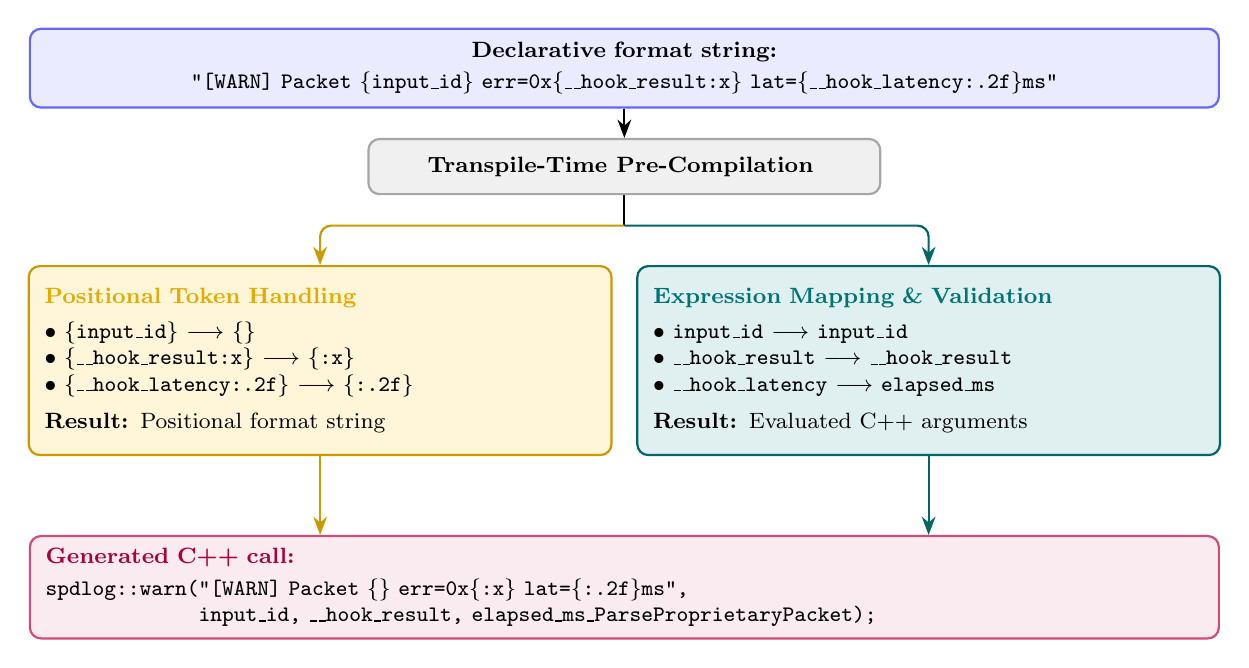
\begin{tikzpicture}[
		>=Stealth,
		font=\footnotesize,
		base/.style={draw, rounded corners=4pt, align=center, thick},
		inputbox/.style={base, fill=blue!8, draw=blue!60, minimum width=15.1cm, text width=14.7cm, minimum height=1.0cm},
		parser/.style={base, fill=gray!12, draw=gray!70, minimum width=6.5cm, minimum height=0.7cm},
		streamA/.style={base, fill=amber!15, draw=amber!80!black, minimum width=7.4cm, text width=7.0cm, minimum height=2.4cm, align=left},
		streamB/.style={base, fill=teal!12, draw=teal!80!black, minimum width=7.4cm, text width=7.0cm, minimum height=2.4cm, align=left},
		outputbox/.style={base, fill=purple!8, draw=purple!70, minimum width=15.1cm, minimum height=1.3cm, text width=14.7cm, align=left},
		tag/.style={font=\bfseries\scriptsize}
	]

		% 1. Input Box
		\node[inputbox] (input) at (0, 0) {
			\textbf{Declarative format string:}\\[2pt]
			\texttt{"[WARN] Packet \{input\_id\} err=0x\{\_\_hook\_result:x\} lat=\{\_\_hook\_latency:.2f\}ms"}
		};

		% 2. Transpiler Parser
		\node[parser] (parser) at (0, -1.25) {
			\textbf{Transpile-Time Pre-Compilation}
		};

		% 3. Dual Streams (Bifurcation)
		\node[streamA, anchor=north east] (streamA) at (-0.15, -2.5) {
			\textbf{\color{amber!90!black}Positional Token Handling}\\[3pt]
			$\bullet$ \texttt{\{input\_id\}} $\longrightarrow$ \texttt{\{\}}\\
			$\bullet$ \texttt{\{\_\_hook\_result:x\}} $\longrightarrow$ \texttt{\{:x\}}\\
			$\bullet$ \texttt{\{\_\_hook\_latency:.2f\}} $\longrightarrow$ \texttt{\{:.2f\}}\\[4pt]
			\textbf{Result:} Positional format string
		};

		\node[streamB, anchor=north west] (streamB) at (0.15, -2.5) {
			\textbf{\color{teal!90!black}Expression Mapping \& Validation}\\[3pt]
			$\bullet$ \texttt{input\_id} $\longrightarrow$ \texttt{input\_id}\\
			$\bullet$ \texttt{\_\_hook\_result} $\longrightarrow$ \texttt{\_\_hook\_result}\\
			$\bullet$ \texttt{\_\_hook\_latency} $\longrightarrow$ \texttt{elapsed\_ms}\\[4pt]
			\textbf{Result:} Evaluated C++ arguments
		};

		% 4. Converged Output
		\node[outputbox, anchor=north] (output) at ([yshift=-1.0cm]0,0 |- streamA.south) {
			\textbf{\color{purple!90!black}Generated C++ call:}\\[2pt]
			\texttt{spdlog::warn("[WARN] Packet \{\} err=0x\{:x\} lat=\{:.2f\}ms",}\\
			\texttt{\phantom{spdlog::warn(}input\_id, \_\_hook\_result, elapsed\_ms\_ParseProprietaryPacket);}
		};

		% Arrows
		\draw[->, thick] (input.south) -- (parser.north);
		
		% Branching from parser to dual streams
		\coordinate (fork) at (0, -2.0);
		\draw[thick] (parser.south) -- (fork);
		\draw[->, thick, rounded corners=4pt, draw=amber!80!black] (fork) -| (streamA.north);
		\draw[->, thick, rounded corners=4pt, draw=teal!80!black] (fork) -| (streamB.north);

		% Downward feeds into output box
		\draw[->, thick, draw=amber!80!black] (streamA.south) -- (streamA.south |- output.north);
		\draw[->, thick, draw=teal!80!black] (streamB.south) -- (streamB.south |- output.north);

	\end{tikzpicture}
	\caption{Transpile-time format string pre-compilation}
	\label{fig:expr_translation_pipeline}
\end{figure}

At runtime, the template emits an spdlog log via \texttt{spdlog::<level>(format\_str, args...)}.
Format string parsing and argument type checking are executed entirely at C++ compile time by \texttt{fmtlib}, resulting in zero runtime parsing overhead within the detour function execution.

Because telemetry frequently evaluates function outcome codes (\texttt{\_\_hook\_result}), elapsed execution latency, and mutated output buffers (\texttt{output\_}), HookDesigner positions the telemetry evaluation block (\texttt{\_telemetry\_body.cpp}) in the hook epilogue, immediately following the trampoline invocation.


\cref{lst:generated_telemetry_cpp} demonstrates the C++ code generated by the transpiler from declarative telemetry rules:

\begin{lstlisting}[language=C++, caption={Generated C++ code inside \texttt{\_hook\_body.cpp} and \texttt{\_telemetry\_body.cpp} demonstrating demand-driven parameter capture and log rule evaluation.}, label={lst:generated_telemetry_cpp}, basicstyle=\ttfamily\footnotesize, breaklines=true]
// --- Entry Parameter Capturing  ---
double input_payloadValue = {};
std::string input_responseBuffer = {};
try {
    input_payloadValue = ReadPointer(payloadValue);
    input_responseBuffer = CopyString(responseBuffer);
    
    ProcessCommandSignal_pre(payloadValue);
} catch (...) {
    OutputDebugStringA("[HOOK EXCEPTION] Exception in pre-hook\n");
}

LARGE_INTEGER start_time_ParseProprietaryPacket;
QueryPerformanceCounter(&start_time_ParseProprietaryPacket);

int __hook_result = TrueParseProprietaryPacket(packetBuffer, complexityWeight);

LARGE_INTEGER end_time_ParseProprietaryPacket;
QueryPerformanceCounter(&end_time_ParseProprietaryPacket);
double elapsed_ms_ParseProprietaryPacket = (double)(end_time_ParseProprietaryPacket.QuadPart - start_time_ParseProprietaryPacket.QuadPart) * 1000.0 / (double)g_PerfFrequency.QuadPart;

try {
    ProcessCommandSignal_post(__hook_result, responseBuffer);

    // Exit Parameter Capturing
    double output_payloadValue = ReadPointer(payloadValue);
    std::string output_responseBuffer = CopyString(responseBuffer);
	
    // Telemetry Evaluation
    if (__hook_result != 200) {
        spdlog::warn("[WARN] Signal failed | id={} | payload: {:.1f} -> {:.1f} | resp: '{}' -> '{}' | lat={:.2f}ms",
                     cmdId,
                     input_payloadValue,
                     output_payloadValue,
                     input_responseBuffer,
                     output_responseBuffer,
                     elapsed_ms_ProcessCommandSignal);
    }
} catch (...) {
    OutputDebugStringA("[HOOK EXCEPTION] Exception in post-hook\n");
}
\end{lstlisting}

\subsection{Static Semantic Validation}
\label{subsec:static_semantic_validation}

During Stage~2 (\texttt{validate\_policy}), HookDesigner performs semantic analysis across declared telemetry rules to catch possible errors offline before DLL compilation.
Beyond standard syntactic checks (such as verifying unique rule identifiers and the mutual exclusivity of \texttt{arguments} and \texttt{format}), the transpiler enforces semantic constraints:

\begin{enumerate}
	\item \textbf{Non-Returning Functions:}
	For target routines classified as non-returning (\texttt{is\_noreturn: true}), execution never returns after trampoline invocation.
	The validator statically rejects any telemetry specification on these targets that references post-invocation properties (including \texttt{execution\_time: true}, \texttt{latency}, \texttt{output\_<param>}, or \texttt{\_\_hook\_result}), preventing the generation of dead code.
	
	\item \textbf{Custom Histogram Buckets Monotonicity:}
	Prometheus registry initialization fails at runtime if histogram bucket upper bounds are unordered or non-positive.
	The transpiler checks custom \texttt{buckets} arrays at compile time to ensure strict positive monotonicity, preventing silent runtime metric registration.
	
	\item \textbf{Bounded Metric Cardinality:}
	A possible failure in metric framework is \emph{cardinality explosion}: the unbounded allocation of metric series caused by assigning high-cardinality values to metric labels or by specifying a huge number of different label per metric.
	HookDesigner strictly restricts metric definitions to at most a single dynamic label, redirecting high-cardinality inspection to structured log events.
\end{enumerate}

\subsection{Asynchronous Logging}
\label{subsec:async_logging}

Logging in high performance environment can be subjected to timing constraints.
Standard synchronous logging models serialize execution by acquiring shared locks and performing blocking operations (such as disk writes or network system calls) directly on the critical execution path.
In an industrial process where intercepted APIs are invoked at high frequencies across multiple threads, synchronous logging often introduces stalls in worker threads, degrading performances of the software under observation.

\subsubsection{Ring Buffer Architecture}

HookDesigner prevents this possible overhead by integrating asynchronous logging powered by \texttt{spdlog}.
During hook initialization in \texttt{\_telemetry\_init.cpp}, the framework pre-allocates an asynchronous thread pool:
\begin{lstlisting}[language=C++, basicstyle=\ttfamily\footnotesize]
spdlog::init_thread_pool(65536, 1);
\end{lstlisting}

This initializes a pre-allocated circular queue capable of holding up to an arbitrary number of pending log items (in our case is $65{,}536$), consumed by a dedicated background worker thread, as modeled in \cref{fig:async_logging_arch}.

\begin{figure}[H]
	\centering
	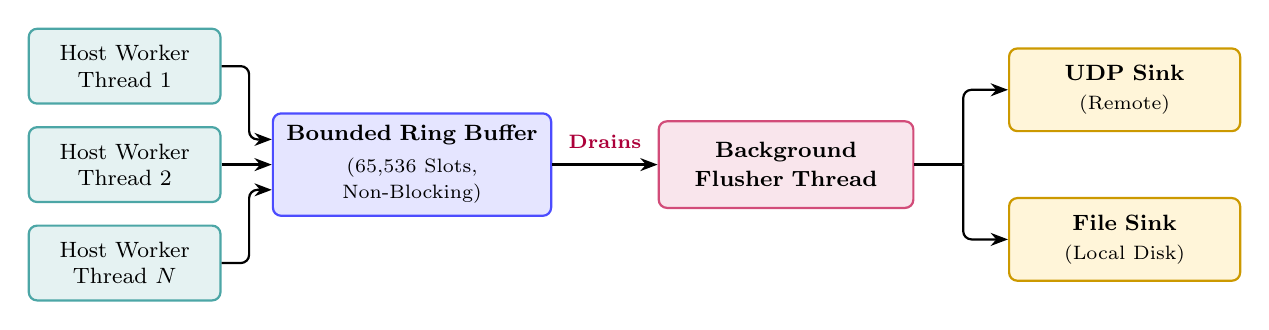
\begin{tikzpicture}[
		font=\footnotesize,
		base/.style={draw, rounded corners=3pt, align=center, thick},
		worker/.style={base, fill=teal!10, draw=teal!70, minimum width=2.4cm, text width=2.2cm, minimum height=0.95cm},
		queue/.style={base, fill=blue!10, draw=blue!70, minimum width=3.5cm, text width=3.3cm, minimum height=1.3cm},
		flusher/.style={base, fill=purple!10, draw=purple!70, minimum width=3.2cm, text width=3.0cm, minimum height=1.1cm},
		sink/.style={base, fill=amber!15, draw=amber!80!black, minimum width=2.9cm, text width=2.7cm, minimum height=1.05cm},
		arrow/.style={-{Stealth[length=2.2mm]}, thick}
	]
		% 1. Host Worker Threads (Producers)
		\node[worker] (th1) at (0, 1.25) {Host Worker\\ Thread 1};
		\node[worker] (th2) at (0, 0)     {Host Worker\\ Thread 2};
		\node[worker] (th3) at (0, -1.25) {Host Worker\\ Thread $N$};

		% 2. Bounded Circular Ring Buffer
		\node[queue] (ring) at (3.65, 0) {\textbf{Bounded Ring Buffer}\\[2pt]\scriptsize (65,536 Slots, Non-Blocking)};

		% 3. Dedicated Background Flusher (1.4cm gap after ring buffer)
		\node[flusher] (bg) at (8.4, 0) {\textbf{Background}\\[1pt]\textbf{Flusher Thread}};

		% 4. Log Sinks
		\node[sink] (udp)  at (12.7, 0.95)  {\textbf{UDP Sink}\\[1pt]\scriptsize  (Remote)};
		\node[sink] (file) at (12.7, -0.95) {\textbf{File Sink}\\[1pt]\scriptsize (Local Disk)};

		% Producer Arrows into Ring Buffer
		\draw[arrow, rounded corners=3pt] (th1.east) -- ++(0.35, 0) |- ([yshift=0.32cm]ring.west);
		\draw[arrow] (th2.east) -- (ring.west);
		\draw[arrow, rounded corners=3pt] (th3.east) -- ++(0.35, 0) |- ([yshift=-0.32cm]ring.west);

		% Queue to Consumer with clear label headroom
		\draw[arrow] (ring.east) -- node[midway, above=2pt, font=\scriptsize\bfseries, color=purple!90!black] {Drains} (bg.west);

		% Consumer to Sinks with clean orthogonal rightward branch
		\coordinate (split) at (10.65, 0);
		\draw[thick] (bg.east) -- (split);
		\draw[arrow, rounded corners=3pt] (split) |- (udp.west);
		\draw[arrow, rounded corners=3pt] (split) |- (file.west);
	\end{tikzpicture}
	\caption{Architecture of the asynchronous structured logging subsystem}
	\label{fig:async_logging_arch}
\end{figure}

When a hook function triggers a log rule, the application thread executes only the minimal CPU instructions required to format the argument tuple and push the record into the circular queue.
No disk I/O, network transmission occurs on the application thread.
The dedicated background thread drains records from the queue and transmits them to the active sinks, guaranteeing that logging overhead on the host threads remains strictly bounded to memory speed.

\subsubsection{Buffer Saturation Policy}

Under burst load, if an application thread generates log messages faster than the background thread can write them to disk or network, a standard logging system will  block the calling thread until queue space becomes available (inducing overhead).
With a pre-allocated capacity of $65{,}536$ ($2^{16}$) entries, the circular ring buffer is intentionally oversized, easily handling standard industrial traffic burst without dropping a single event.
Saturating a queue of this size is unlikely under normal operating conditions; it represents extreme scenario---such as complete physical disk stalls or total network interface disconnection.
In the rare event that saturation does occur, HookDesigner avoids this by configuring the asynchronous logger with the \texttt{overrun\_oldest} policy:
\begin{lstlisting}[language=C++, basicstyle=\ttfamily\footnotesize]
spdlog::async_overflow_policy::overrun_oldest
\end{lstlisting}
Under queue saturation, if the $65{,}536$-entry queue fills completely, the logger drops the oldest unwritten messages to make space for incoming events.
This guarantees that application worker threads are \emph{never} blocked by logs operations, following the minimal-overhead telemetry design principle established in \cref{sec:arch_overview}.

\subsubsection{Network and Storage Sinks}

The logging subsystem supports two distinct log destination (sink):
\begin{itemize}
	\item \textbf{UDP Sink (\texttt{logger\_config.type: "udp"})}:
	Industrial deployments frequently aggregate telemetry across distributed nodes into monitoring systems (such as Promtail, Grafana Loki).
	HookDesigner integrates a non-blocking UDP sink using \texttt{spdlog::}\allowbreak\texttt{sinks::}\allowbreak\texttt{udp\_sink\_mt}.
	Log messages are formatted according to RFC-5424 Syslog specifications:
	\begin{lstlisting}[language=C++, basicstyle=\ttfamily\footnotesize]
logger->set_pattern("<165>1 %Y-%m-%dT%H:%M:%SZ host scada_hook - - - %v");
	\end{lstlisting}
	Utilizing connectionless \ac{UDP} transport provides a reliability advantage: if the remote logging server crashes or network connectivity is severed, the operating system kernel immediately discards the packets.
	The hook payload never blocks attempting to re-establish TCP handshakes, isolating the host process from external network failures.

	\item \textbf{Local File Sink (\texttt{logger\_config.type: "file"}):}
	HookDesigner instantiates also a asynchronous basic file sink (\texttt{spdlog::sinks::basic\_file\_sink\_mt}).
	File flushing is explicitly triggered only on error conditions (\texttt{spdlog::flush\_on(spdlog::level::err)}) to minimize disk write amplification during a possible host process crash.
\end{itemize}

\subsection{Performance Metrics Engine}
\label{subsec:prometheus}

While asynchronous logging provides textual event traces, monitoring of industrial software requires also quantitative analysis (e.g. request throughput, error ratios, and latency distributions).
Extracting these data from log streams requires external log parsing, which could be computationally expensive.

To provide \emph{instantaneous} quantitative observability, HookDesigner integrates Prometheus metrics exposition via \texttt{prometheus-cpp}.
The instrumentation payload hosts an embedded Prometheus HTTP server that continuously exposes current metric values to external scrapers.

\subsubsection{Registration and Metric Family Hierarchy}

During hook payload initialization (\texttt{InitializeHooks}), the framework allocates a global metric registry and starts an embedded CivetWeb-based HTTP exposer on the configured socket address:
\begin{lstlisting}[language=C++, basicstyle=\ttfamily\footnotesize]
g_PromRegistry = std::make_shared<prometheus::Registry>();
g_PromExposer = std::make_unique<prometheus::Exposer>("telemetry.metrics_config.endpoint");
g_PromExposer->RegisterCollectable(g_PromRegistry);
\end{lstlisting}

For every metric declared under \texttt{behaviors.performance\_metrics}, HookDesigner generates typed global metric family pointers (\texttt{g\_PromFamily\_<Function>\_<Metric>}) bound to the central registry:
\begin{itemize}
	\item \textbf{Counters (\texttt{BuildCounter}):} Monotonically increasing values used to track event frequencies (e.g., total packets processed, errors encountered).
	\item \textbf{Gauges (\texttt{BuildGauge}):} Arbitrary numerical values that can increase or decrease, representing instantaneous states (e.g., active queue depth, buffer capacity).
	\item \textbf{Histograms (\texttt{BuildHistogram}):} Samples observations into configurable statistical buckets alongside cumulative counts and sums
\end{itemize}

\subsubsection{Dynamic Labels}
\label{subsubsec:metric_labels}

Prometheus metrics achieve multi-dimensional data modeling through key-value labels.
Intercepted function calls rarely carry uniform monitored value; an analyst must differentiate observations based on runtime execution context (e.g. distinguishing normal completions from error codes, tracking request w.r.t. specific value of a variable).

Without labels, an analyst would be forced to define separate, metric families for every potential outcome (e.g., \texttt{packets\_success\_total}, \texttt{packets\_auth\_error\_total}, \texttt{packets\_crc\_error\_total}).
This practice pollutes the metric registry and requires continuous re-compilation whenever new statuses arise.
By attaching dynamic labels (e.g., \texttt{packets\_total\{status="success"\}}), a single metric family can be dynamically partitioned at runtime according to the specified key (variable).

\paragraph{Lock Contention Bottleneck}
\label{subsubsec:lock_contention}

While dynamic labels provide monitoring dynamic granularity, implementing them efficiently presents a performance challenge.
In the standard \texttt{prometheus-cpp} library, observing a metric with dynamic labels requires invoking:
\begin{lstlisting}[language=C++, basicstyle=\ttfamily\footnotesize]
family->Add({ {"label_key", label_value} }).Increment();
\end{lstlisting}
Under the hood, \texttt{prometheus::Family<T>::Add()} maintains an internal structure protected by a lock.
Every time a hook executes an observation, the thread must:
\begin{enumerate}
	\item Construct a node containing the label key-value pair, triggering heap allocations.
	\item Acquire the family's internal lock.
	\item Perform an associative tree search across registered label sets.
	\item Release the lock and return the metric reference.
\end{enumerate}

In a multi-threaded application where worker threads execute thousands of operations per second, this design induces \emph{lock contention}.
Threads serialize on the shared lock, introducing latency into the host application.

\paragraph{The Lock-Free Thread-Local Cache}

HookDesigner overcomes this bottleneck by implementing a \emph{Caching strategy} generated into \texttt{\_telemetry\_body.cpp}.

Behind this optimization is \emph{temporal label locality}: within industrial processes, worker threads frequently execute batches of operations that share identical label values over extended time windows (e.g., a worker thread processing consecutive packets belonging to the same connection ID).

To exploit this locality, the transpiler generates two thread-local variables for every labeled metric, accessible without acquiring any lock:
\begin{enumerate}
	\item \texttt{thread\_local uint64\_t tl\_last\_hash}: Stores the 64-bit hash of the last observed label value on that specific thread.
	\item \texttt{thread\_local MetricType* tl\_last\_ptr}: Stores a direct pointer to the underlying Prometheus metric instance.
\end{enumerate}

\cref{lst:pod_cache_listing} illustrates the caching logic generated by the transpiler.

\begin{lstlisting}[language=C++, caption={Zero-lock thread-local caching mechanism}, label={lst:pod_cache_listing}, basicstyle=\ttfamily\footnotesize, breaklines=true]
if (g_PromFamily_ParseProprietaryPacket_packets_total) {
    if (__hook_result == 1) {
        // Evaluate label string and compute 64-bit hash
        std::string cur_val = ToLabelString("success");
        uint64_t cur_hash = std::hash<std::string>{}(cur_val);

        // Thread-local storage variables
        thread_local uint64_t tl_last_hash_packets_total = 0;
        thread_local prometheus::Counter* tl_last_ptr_packets_total = nullptr;

        // Fast-Path Check: bypass mutex if label matches cached state
        if (tl_last_ptr_packets_total == nullptr || tl_last_hash_packets_total != cur_hash) {
            // SLOW PATH: Mutex acquired only on start or label transition
            tl_last_ptr_packets_total = &g_PromFamily_ParseProprietaryPacket_packets_total->Add({ {"status", cur_val} });
            tl_last_hash_packets_total = cur_hash;
        }

        // FAST PATH: Lock-free atomic increment
        tl_last_ptr_packets_total->Increment();
    }
}
\end{lstlisting}

\subsubsection{Direct Binding for Label-less Metrics}

For metrics defined without dynamic labels, HookDesigner applies a compile-time optimization.
Because the metric dimensionality is static, resolving the metric instance dynamically at runtime is entirely redundant.
During initialization (\texttt{\_telemetry\_init.cpp}), the transpiler generatess code that registers the metric family and immediately adds the base instance, storing the result in a static global pointer:
\begin{lstlisting}[language=C++, basicstyle=\ttfamily\footnotesize]
g_PromMetric_ParseProprietaryPacket_total = &g_PromFamily_ParseProprietaryPacket_total->Add({ {"function", "ParseProprietaryPacket"} });
\end{lstlisting}

Inside the hook function (\texttt{\_telemetry\_body.}\allowbreak\texttt{cpp}), the observation bypasses even the thread-local hash check, updating the metric directly through the global pointer:
\begin{lstlisting}[language=C++, basicstyle=\ttfamily\footnotesize]
if (g_PromMetric_ParseProprietaryPacket_total) {
    g_PromMetric_ParseProprietaryPacket_total->Increment();
}
\end{lstlisting}
This delivers maximum execution efficiency, reducing metric recording overhead to a single atomic instruction.

To demonstrate how these heterogeneous telemetry features operate cohesively within an intercepted function, \cref{lst:telemetry_summary_cpp} illustrates the complete in-hook telemetry evaluation block generated with \texttt{\_telemetry\_body.cpp}.
In this example we can see spdlog logging, counters, cached labeled histograms, and state gauges that HookDesigner handle with minimal overhead.

\begin{lstlisting}[language=C++, caption={Generated in-hook telemetry block (\texttt{\_telemetry\_body.cpp}) illustrating the co-existence of the seen telemetry features}, label={lst:telemetry_summary_cpp}, basicstyle=\ttfamily\footnotesize, breaklines=true]
	// Asynchronous Logging
	if (__hook_result != 1) {
		spdlog::warn("[WARN] Dispatch failed | id={} | code={} | lat={:.2f}ms",
		input_packetId, 
		__hook_result, 
		elapsed_ms_DispatchPacket);
	}

	// Metric Update (No label)
	if (g_PromMetric_DispatchPacket_invocations_failed) {
		if (__hook_result != 1) {
			g_PromMetric_DispatchPacket_invocations_failed->Increment();
		}
	}
	
	// Dynamic-Label Histogram
	if (g_PromFamily_DispatchPacket_latency_ms) {
		std::string cur_val = ToLabelString(__hook_result == 1 ? "success" : "failure");
		uint64_t cur_hash = std::hash<std::string>{}(cur_val);
		
		thread_local uint64_t tl_last_hash_latency_ms = 0;
		thread_local prometheus::Histogram* tl_last_ptr_latency_ms = nullptr;
		
		if (tl_last_ptr_latency_ms == nullptr || tl_last_hash_latency_ms != cur_hash) {
			tl_last_ptr_latency_ms = &g_PromFamily_DispatchPacket_latency_ms->Add(
			{ {"status", cur_val} }, 
			g_PromBuckets_DispatchPacket_latency_ms
			);
			tl_last_hash_latency_ms = cur_hash;
		}
		tl_last_ptr_latency_ms->Observe(elapsed_ms_DispatchPacket);
	}
	
	// Gauge
	if (g_PromMetric_DispatchPacket_queue_depth) {
		g_PromMetric_DispatchPacket_queue_depth->Set((double)(g_active_queue_depth.load()));
	}
\end{lstlisting}



\section{Hook Function Safety}
\label{sec:safety_fault_tolerance}

As we have seen in \cref{subsec:address_space_isolation}, during binary instrumentation, the compiled payload runs directly inside the target application's virtual address space without any isolation boundary.
While this shared-memory execution model enables the instrumentation, it introduces safety issues: any possible bugs in the injected code (user callbacks, telemetry code) can make crash the host application immediately.
In production environments, such unexpected terminations are unacceptable, directly violating the \emph{Crash Safety} design principle established in \cref{subsec:design_principles}.

To satisfy this requirement, HookDesigner incorporates a defensive architecture designed to prevent possible hook crashes:
\begin{enumerate}
	\item \textbf{Asynchronous Exception Handling:} By compiling the payload with the MSVC \texttt{/EHa} model, all the possible exceptions are intercepted and prevented from crashing the host process (\cref{subsec:seh}).
	\item \textbf{Memory Access Helpers:} the transpiler generates safe pointer dereference and string copying helpers that protect argument capturing (\cref{subsec:safe_access}).
	\item \textbf{Thread-Local Recursion Guard:} A TLS guard prevents re-entrant hook execution loops caused by circular API invocations on the same thread (\cref{subsec:recursion_guard}).
	\item \textbf{Complete Hook Function Structure:} this structure shows how the presented defenses are integrated within the definitive Hook Function implementation, with specializations for both standard and non-returning functions (\cref{subsec:hook_pipeline}).
\end{enumerate}

\subsection{Asynchronous Exception Handling}
\label{subsec:seh}

In standard C++ development on Windows, compilers typically use the synchronous exception model (\texttt{/EHsc}).
Under \texttt{/EHsc}, C++ \texttt{try/catch} blocks are designed only to intercept exceptions thrown explicitly through the C++ \texttt{throw} statement.
Under this standard configuration, a C++ \texttt{catch(...)} block does not catch  OS-level faults---such as dereferencing a null pointer, reading an unmapped virtual address, or encountering a division by zero.
In this way, the exception bypasses user code, triggers the default operating system exception filter, and terminates the host process immediately.

\subsubsection{The /EHa Asynchronous Exception Model}

To eliminate this behavior, HookDesigner's compilation enforces the asynchronous exception handling 
by passing the \texttt{/EHa} flag to MSVC (\cref{subsec:compilation}) compiler.
Under \texttt{/EHa}, the compiler generates structured unwinding tables that bridge Windows kernel \ac{SEH} with C++ exception handling:
\begin{itemize}
	\item Standard C++ \texttt{catch(...)} clauses are transformed to catch both synchronous C++ exceptions and asynchronous Win32 hardware faults.
	\item Proper stack unwinding and destructors execution are guaranteed even when an instruction triggers an OS fault.
\end{itemize}

\subsubsection{Exception Boundaries}

HookDesigner leverages the \texttt{/EHa} model by establishing two isolated boundaries inside each hook function in \texttt{\_hook\_body.cpp}:
one enclosing pre-execution logic (including telemetry argument capture and user \texttt{pre\_hook} callbacks), and one enclosing post-execution logic (including user \texttt{post\_hook} callbacks, argument exit capture, and telemetry evaluation).

\cref{lst:seh_boundaries} illustrates this pattern:
\begin{itemize}
	\item If the fault occurs inside the \emph{pre-hook boundary},  the function jumps directly to the original target function via its trampoline.
	The host process continues its normal execution without crashing.
	\item If the fault occurs inside the \emph{post-hook boundary}, the failed callback or telemetry rule is abandoned, and execution returns to the original caller.
\end{itemize}

\begin{lstlisting}[language=C++, caption={Exception boundaries in \texttt{\_hook\_body.cpp}}, label={lst:seh_boundaries}, basicstyle=\ttfamily\footnotesize, breaklines=true]
// Pre-Execution Boundary
try {
    // Parameter capture and user pre-hook
    input_payload = ReadPointer(payloadValue);
    UserPreCallback(payloadValue);
    
} catch (const std::exception& ex) {  //captures standard C++ exceptions
    OutputDebugStringA("[HOOK EXCEPTION] Access violation contained in pre-hook\n");
} 

catch (...) {  //captures also Win32 hardware faults (thanks to the /EHa flag)
    OutputDebugStringA("[HOOK EXCEPTION] Access violation contained in pre-hook\n");
}

int __hook_result = TrueTargetFunction(payloadValue);

// Post-Execution Boundary
try {
    // User post-hook, exit capture, telemetry
    
    UserPostHook(__hook_result);
   
    output_payload = ReadPointer(payloadValue);
    EvaluateTelemetry();
} catch (const std::exception& ex) {
    OutputDebugStringA("[HOOK EXCEPTION] Access violation contained in post-hook\n");

} catch (...) {
    OutputDebugStringA("[HOOK EXCEPTION] Access violation contained in post-hook\n");
}

return __hook_result;
\end{lstlisting}

\subsection{Transpiler Type Analysis and Memory Access Helpers}
\label{subsec:safe_access}

As already explained in \cref{subsec:param_capture}, binary instrumentation authors often need to inspect function parameters on function entry and exit.
However, manually writing C++ code to capture parameters' value is error-prone: forgetting a null check, dereferencing an invalid pointer, or traversing an unbounded string can easily cause memory access violations.
To help the work of policy authors, HookDesigner \emph{automates} access to primitive variables and strings in a safe way.
By analyzing parameter types at transpile time, the framework automatically generates the appropriate access solution, preventing the author from writing repetitive and error-prone C++ boilerplate.

\subsubsection{Type Analysis}

As introduced in \cref{subsec:param_capture}, every parameter required for telemetry must be safely captured on function entry or exit.
To automate this without requiring manual boilerplate from the user, the transpiler performs static type analysis on each parameter's Clang type representation (preserved from the Stage~1 in \cref{subsec:libclang_ast}).

The analysis classifies each parameter through three conceptual phases:
\begin{itemize}
	\item \textbf{Canonical Alias Resolution:} In C and Win32 development, types are frequently masked behind typedefs (such as \texttt{DWORD}, \texttt{LPSTR}, or \texttt{size\_t}). The transpiler traverses \texttt{get\_canonical()} to resolve these aliases to their underlying primitive representation.
	\item \textbf{Pointer Indirection Resolution:} By recursively unwinding pointee types, the transpiler calculates the pointer depth $d$. Types with $d = 1$ pointing to character types (\texttt{char}, \texttt{wchar\_t}) are classified as string candidates, whereas non-pointer primitives have $d = 0$.
	\item \textbf{Safe Access Expression:} For string pointers, the transpiler generates safe copy calls (\texttt{CopyString}). For dereferenceable primitive pointers (excluding opaque handles such as \texttt{void*} and complex structures), it nests $d$ dereference helpers (\texttt{ReadPointer}). Opaque handles and direct values are passed unchanged.
\end{itemize}

This automated classification enables the transpiler to emit uniform assignments of the form \texttt{input\_<p> = safe\_read\_expr} without requiring template branching in the hook body.
\cref{tab:type_analysis_matrix} formalizes the complete type mapping matrix.

\begin{table}[H]
	\centering
	\small
	\begin{tabularx}{\textwidth}{@{} p{2.8cm} c p{2.5cm} >{\RaggedRight}X p{2.4cm} @{}}
		\toprule
		\textbf{Clang Type} & \textbf{Depth ($d$)} & \textbf{Category} & \textbf{Generated Read Expression} & \textbf{Storage Type} \\
		\midrule
		\texttt{int}, \texttt{double}, \texttt{DWORD} & 0 & Primitive Value & \texttt{param} & \texttt{T} (original type) \\
		\addlinespace
		\texttt{const char*}, \texttt{char*} & 1 & C-String & \texttt{CopyString(param)} & \texttt{std::string} \\
		\addlinespace
		\texttt{const wchar\_t*}, \texttt{wchar\_t*} & 1 & Wide C-String & \texttt{CopyString(param)} & \texttt{std::string} (UTF-8) \\
		\addlinespace
		\texttt{int*}, \texttt{double*} & 1 & Primitive Pointer & \texttt{ReadPointer(param)} & Underlying type (\texttt{int}) \\
		\addlinespace
		\texttt{int**} & 2 & Nested Pointer & \texttt{ReadPointer(}\allowbreak\texttt{ReadPointer(param))} & Underlying type (\texttt{int}) \\
		\addlinespace
		\texttt{void*}, \texttt{HANDLE} & 1 & Opaque Handle & \texttt{param} & Raw pointer type \\
		\bottomrule
	\end{tabularx}
	\caption{Mapping clang type and generated expression}
	\label{tab:type_analysis_matrix}
\end{table}

\subsubsection{Memory-Safety Helper Functions}

Most of the generated expressions leverage helper functions defined in \texttt{\_user\_logic\_}\allowbreak\texttt{helpers.cpp}:

\begin{itemize}
	\item \textbf{Pointer Dereferencing (\texttt{ReadPointer<T>}):}
	When reading data through a pointer, standard C++ dereferencing (\texttt{*ptr}) crashes the process if the pointer is null or unmapped.
	HookDesigner defines a templated helper:
	\begin{lstlisting}[language=C++, basicstyle=\ttfamily\footnotesize]
template <typename T>
static T ReadPointer(const T* ptr, T fallback = T()) {
    if (!ptr) {
        return fallback;
    }
    return *ptr;
}
	\end{lstlisting}
	If \texttt{ptr} is null, \texttt{ReadPointer} returns the default-constructed fallback value without attempting a dereference.
	If \texttt{ptr} contains a non-null but unmapped address (e.g., a dangling pointer pointing to deallocated memory), the resulting read violation is trapped by the outer \texttt{/EHa} exception boundary.

	\item \textbf{Bounded String Copying (\texttt{CopyString}):}
	Passing raw string pointers (\texttt{char*} or \texttt{wchar\_t*}) directly to logging formatters is dangerous: if the target buffer lacks a null terminator or points to invalid memory, formatting routines read past the buffer boundary until they fault.
	HookDesigner generates explicit calls to \texttt{CopyString}:
	\begin{lstlisting}[language=C++, basicstyle=\ttfamily\footnotesize]
static std::string CopyString(const char* source, size_t maxChars = 128) {
    if (!source) return "null";
    size_t len = strnlen(source, maxChars);
    return std::string(source, len);
}
	\end{lstlisting}
	\texttt{CopyString} checks for null pointers, returning the literal \texttt{"null"}.
	For valid pointers, it uses the bounded length function \texttt{strnlen(source, maxChars)}, reading at most 128 characters.
	For wide strings (\texttt{wchar\_t*}), an overloaded implementation uses \texttt{wcsnlen} and converts the result to UTF-8 using \texttt{WideCharToMultiByte(CP\_UTF8)}, ensuring consistent log formatting.
\end{itemize}

\subsubsection{Member Access Contract}

As introduced in \cref{subsec:param_capture}, when a policy rule references an internal struct member using the arrow or dot operator (e.g., \texttt{\{input\_pQueue->queueId\}}), the transpiler detects the operator and \emph{bypasses automated Clang type analysis} on the accessed field.
Instead, it emits the member access expression defined in the YAML policy directly into the generated C++ code.

This design establishes an explicit contract:
\begin{itemize}
	\item \textbf{Author Flexibility:} The policy author can inspect  nested member field, HookDesigner will not refuse the policy.
	\item \textbf{Author Responsibility:} The author is responsible for ensuring pointer or string member safety from the YAML policy, exploiting the helpers provided in \texttt{logic\_helpers.cpp} (e.g. by wrapping the expression in \texttt{ReadPointer(}\allowbreak\texttt{input\_pQueue->queueId)} if the field \texttt{queueId} is a pointer).
	\item \textbf{Exception Boundary Safety:} However, any possible error of the policy author is intercepted by the outer \texttt{/EHa} SEH containment boundary, preventing any possible host crash.
\end{itemize}

\subsection{Recursion Guard}
\label{subsec:recursion_guard}

In binary instrumentation, a common cause of unexpected process termination is \emph{hook re-entrancy}.
Because hooks are installed globally at the entry point of target APIs, any code executed inside the hook payload that directly or indirectly calls a hooked function can trigger an infinite loop on the calling thread.

\subsubsection{The Re-Entrancy Mechanism}

Let's consider an instrumentation configuration where the \texttt{WriteFile} API is hooked.
When the host application invokes \texttt{WriteFile}, execution jumps to the hook function.
Inside the function, a logging rule or diagnostic trace might call a utility that writes a debug string to a file or invokes an internal logging routine that ultimately calls \texttt{WriteFile}.
Without re-entrancy protection, this second call re-enters the hook function from the beginning, which again triggers the logger, forming an infinite recursion loop:
$$\text{HookedWriteFile} \longrightarrow \text{Log} \longrightarrow \text{WriteFile} \longrightarrow \text{HookedWriteFile} \longrightarrow \dots$$
Because each nested invocation allocates a new stack frame, the thread stack is rapidly consumed.
Stack overflow generates a \texttt{STACK\_OVERFLOW} exception, terminating the host application.

\subsubsection{The RecursionHookGuard Definition}

HookDesigner eliminates the re-entrancy risk through a per-thread 
guard.
During hook payload initialization (\texttt{InitializeHooks}), the framework allocates a process-wide TLS slot index:
\begin{lstlisting}[language=C++, basicstyle=\ttfamily\footnotesize]
static DWORD g_TlsIndex = TLS_OUT_OF_INDEXES;
// Inside InitializeHooks():
g_TlsIndex = TlsAlloc();
\end{lstlisting}

Using this slot, HookDesigner implements a RAII helper structure named \texttt{RecursionHookGuard} in the helper file \texttt{\_user\_logic\_helpers.cpp}, shown in \cref{lst:recursion_guard}:

\begin{lstlisting}[language=C++, caption={\texttt{RecursionHookGuard} RAII implementation in \texttt{\_user\_logic\_helpers.cpp}.}, label={lst:recursion_guard}, basicstyle=\ttfamily\footnotesize, breaklines=true]
struct RecursionHookGuard {
    bool active;
    RecursionHookGuard() : active(false) { Acquire(); }
    ~RecursionHookGuard() { Release(); }

    void Acquire() {
        if (!active) {
            TlsSetValue(g_TlsIndex, (LPVOID)1);
            active = true;
        }
    }

    void Release() {
        if (active) {
            TlsSetValue(g_TlsIndex, (LPVOID)0);
            active = false;
        }
    }
};
\end{lstlisting}

\subsubsection{The New Hook Function Control Flow}

As shown in \cref{fig:recursion_flowchart}, at the entry of each generated hook function (\texttt{Hooked<F>}), before executing any code, the function inspects the thread's recursion state:
\begin{lstlisting}[language=C++, basicstyle=\ttfamily\footnotesize]
if (TlsGetValue(g_TlsIndex) != 0) {
    return True<FunctionName>(param1, param2, ...);
}
\end{lstlisting}

If the \ac{TLS} value is non-zero, the thread is already executing inside an active hook function.
The function immediately redirect execution directly to the original trampoline pointer (\texttt{True<FunctionName>}), bypassing all hook logic.

If the thread is not in a recursive call (\texttt{TlsGetValue == 0}), the function instantiates a local \texttt{RecursionHookGuard} on the stack, which sets the \ac{TLS} flag to \texttt{1} (\texttt{Acquire()}).
Crucially, right before invoking the trampoline to execute the original target function, the function calls:
\begin{lstlisting}[language=C++, basicstyle=\ttfamily\footnotesize]
hook_recursion_guard.Release();
\end{lstlisting}

This pre-trampoline release is a deliberate choice:
\begin{itemize}
	\item While user pre-hook and post-hook injected logic execute, the guard is \emph{active} (\texttt{1}), blocking any re-entrant hook loops triggered by callbacks or telemetry code.
	\item While the original target function executes, the guard is \emph{released} (\texttt{0}).
	If the target function legitimately calls \emph{another} hooked function as part of its normal operation, that nested call is permitted to enter its own hook function and be monitored.
\end{itemize}
After the trampoline returns, the function re-acquires the guard (\texttt{hook\_recursion\_guard.}\allowbreak\texttt{Acquire()}) to protect post-hook execution and telemetry recording.

Finally, when the hook function completes and returns, \texttt{hook\_recursion\_guard} goes out of scope on the stack.
Its RAII destructor automatically invokes \texttt{Release()}, restoring the \ac{TLS} slot to \texttt{0}.
By relying on RAII, even if an unexpected exception occurs at any point during pre-hook or post-hook execution, the stack unwinding mechanism automatically disarms the guard, ensuring the thread is always returned to a fair, non-recursive state.

\begin{figure}[H]
	\centering
	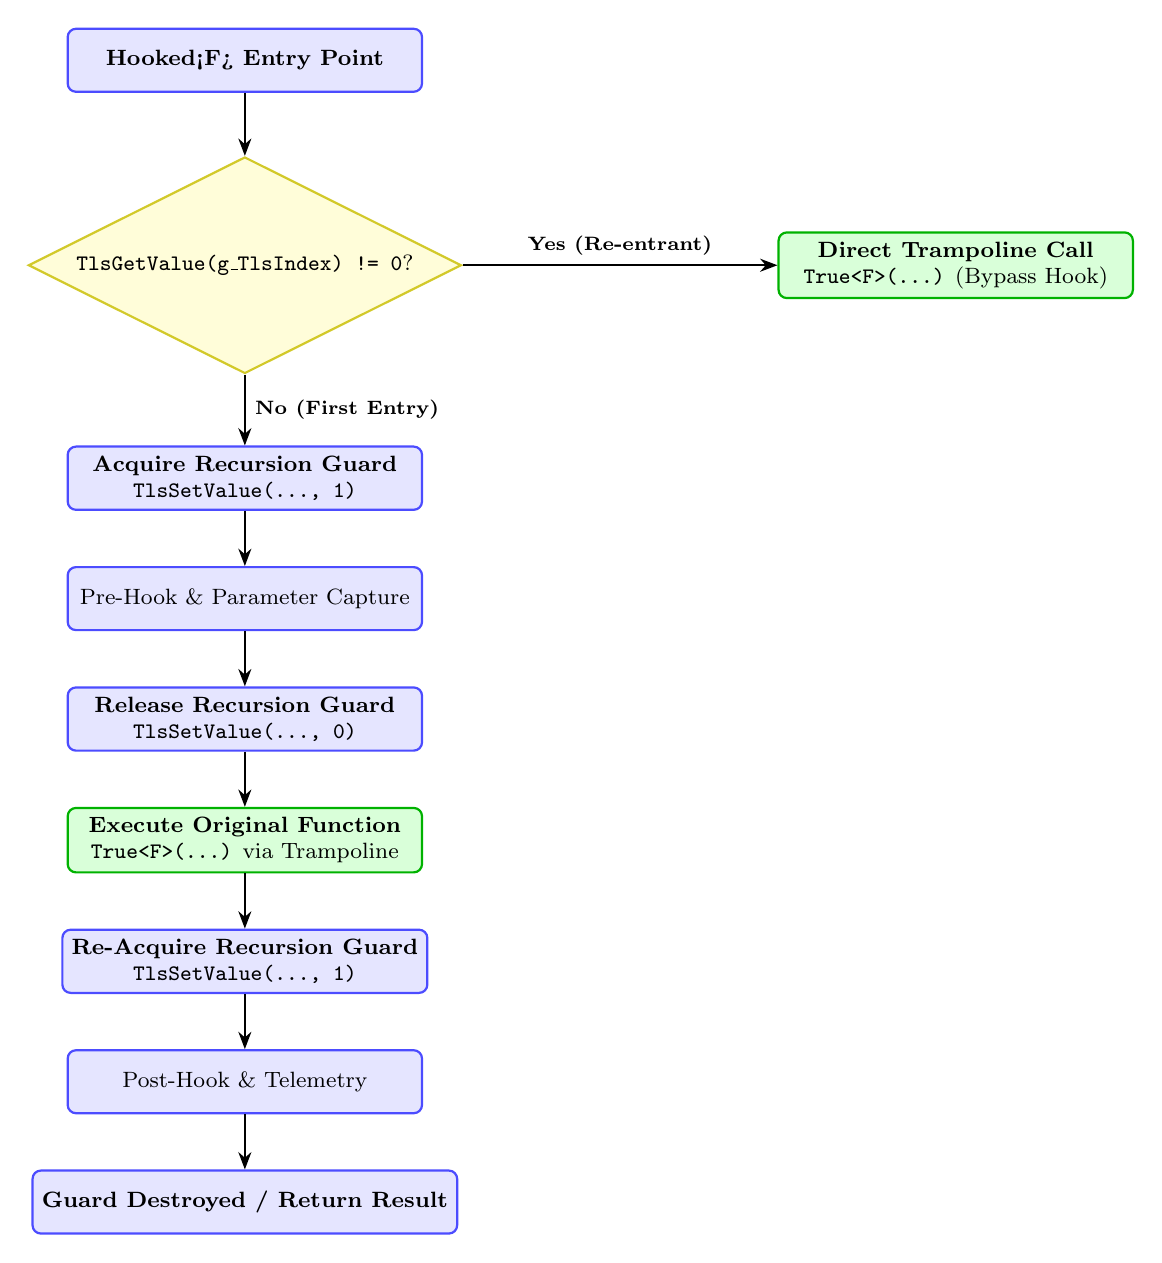
\begin{tikzpicture}[
		>=Stealth,
		font=\footnotesize,
		base/.style={draw, rounded corners=3pt, align=center, thick},
		decision/.style={draw, diamond, aspect=2, align=center, thick, fill=yellow!15, draw=yellow!80!black},
		block/.style={base, fill=blue!10, draw=blue!70, minimum width=4.5cm, minimum height=0.8cm},
		trampoline/.style={base, fill=green!15, draw=green!70!black, minimum width=4.5cm, minimum height=0.8cm},
		arrow/.style={-{Stealth[length=2.2mm]}, thick}
	]
		\node[block] (entry) {\textbf{Hooked<F> Entry Point}};
		\node[decision, below=0.8cm of entry] (check) {\texttt{TlsGetValue(g\_TlsIndex) != 0}?};
		\node[trampoline, right=4.0cm of check] (bypass) {\textbf{Direct Trampoline Call}\\ \texttt{True<F>(...)} (Bypass Hook)};
		\node[block, below=0.9cm of check] (acquire) {\textbf{Acquire Recursion Guard}\\ \texttt{TlsSetValue(..., 1)}};
		\node[block, below=0.7cm of acquire] (pre) {Pre-Hook \& Parameter Capture};
		\node[block, below=0.7cm of pre] (release) {\textbf{Release Recursion Guard}\\ \texttt{TlsSetValue(..., 0)}};
		\node[trampoline, below=0.7cm of release] (orig) {\textbf{Execute Original Function}\\ \texttt{True<F>(...)} via Trampoline};
		\node[block, below=0.7cm of orig] (reacquire) {\textbf{Re-Acquire Recursion Guard}\\ \texttt{TlsSetValue(..., 1)}};
		\node[block, below=0.7cm of reacquire] (post) {Post-Hook \& Telemetry};
		\node[block, below=0.7cm of post] (exit) {\textbf{Guard Destroyed / Return Result}};

		\draw[arrow] (entry) -- (check);
		\draw[arrow] (check) -- node[above, font=\scriptsize\bfseries] {Yes (Re-entrant)} (bypass);
		\draw[arrow] (check) -- node[right, font=\scriptsize\bfseries] {No (First Entry)} (acquire);
		\draw[arrow] (acquire) -- (pre);
		\draw[arrow] (pre) -- (release);
		\draw[arrow] (release) -- (orig);
		\draw[arrow] (orig) -- (reacquire);
		\draw[arrow] (reacquire) -- (post);
		\draw[arrow] (post) -- (exit);
	\end{tikzpicture}
	\caption{Hook control flow with TLS-based recursion guard}
	\label{fig:recursion_flowchart}
\end{figure}

\subsection{The Complete Hook Function Structure}
\label{subsec:hook_pipeline}

All the presented Hook safety features converge in the implementation of the hook function body (\texttt{\_hook\_body.cpp}).
Depending on whether the intercepted target function returns to its caller or is a non-returning function, HookDesigner generates one of two distinct structures: 

\subsubsection{Standard Hook Function Body}

To illustrate how these defenses integrate in practice for standard returning targets, \cref{lst:generated_hook_function} presents a complete generated C++ Hook function.

\begin{lstlisting}[language=C++, caption={Complete generated hook function demonstrating integrated safety mechanisms.}, label={lst:generated_hook_function}, basicstyle=\ttfamily\footnotesize, breaklines=true]
int __stdcall HookedProcessPacket(int packetId, char* payload, double* sensorVal) {
    // Thread Re-Entrancy Check
    if (TlsGetValue(g_TlsIndex) != 0) {
        return TrueProcessPacket(packetId, payload, sensorVal);
    }

    // Thread Guards (TLS Recursion & Active Thread Tracking)
    RecursionHookGuard hook_recursion_guard;
    HookActiveThreads hook_active_threads;

    int input_packetId = {};
    std::string input_payload = {};
    double input_sensorVal = {};

    // Pre-Execution Boundary
    try {
        input_packetId = packetId;
        input_payload = CopyString(payload);
        input_sensorVal = ReadPointer(sensorVal);

        ProcessPacket_pre(packetId, payload);
    } catch (const std::exception& ex) {
        OutputDebugStringA("[HOOK EXCEPTION] Pre-hook error in ProcessPacket\n");
    } catch (...) {
        OutputDebugStringA("[HOOK EXCEPTION] Access violation in pre-hook\n");
    }

    LARGE_INTEGER start_time;
    QueryPerformanceCounter(&start_time);

    // Trampoline Execution (Guard Temporarily Disarmed)
    hook_recursion_guard.Release();
    int __hook_result = TrueProcessPacket(packetId, payload, sensorVal);

    LARGE_INTEGER end_time;
    QueryPerformanceCounter(&end_time);
    double elapsed_ms = (end_time.QuadPart - start_time.QuadPart) * 1000.0 / g_PerfFrequency.QuadPart;

    // Post-Execution Boundary

	//After Trampoline execution, re-acquire guard
    hook_recursion_guard.Acquire();
    try {
        ProcessPacket_post(__hook_result, payload);

        double output_sensorVal = ReadPointer(sensorVal);

        spdlog::info("[PACKET] ID: {}, Latency: {:.2f}ms", input_packetId, elapsed_ms);
        if (g_PromMetric_ProcessPacket_invocations) {
            g_PromMetric_ProcessPacket_invocations->Increment();
        }
    } catch (const std::exception& ex) {
    	OutputDebugStringA("[HOOK EXCEPTION] post-hook error in ProcessPacket\n");
    } 
    catch (...) {
    	OutputDebugStringA("[HOOK EXCEPTION] Access violation in post-hook\n");
    }

    return __hook_result;
}
\end{lstlisting}

\subsubsection{Adaptation for Non-Returning Targets}
\label{subsec:noreturn_adaptation}

The standard hook function body operates on the premise that the intercepted target function eventually returns after execution.
However, several system APIs are \emph{non-returning functions}:
they terminate the thread or process, or transfer control directly to an external exception dispatcher, never returning control to the caller.

If a non-returning function is instrumented using the standard returning function structure, the instrumentation payload encounters the following architectural failures:
\begin{enumerate}
	\item \textbf{Post-Trampoline Telemetry dead-code:} In \_hook\_body.cpp, telemetry evaluation is executed after the trampoline call inside the post-execution block, for this reason it is never reached with this type of functions
	\item \textbf{Bypassed C++ Stack Unwinding:} When a process or thread terminates, the operating system immediately tears down the user-mode execution context.
	Standard C++ stack unwinding is skipped, meaning that local RAII destructors on the stack are \emph{never executed}.
	Consequently, the destructor of \texttt{HookActiveThreads} (\cref{lst:ejection_sync}) never runs, causing the global \texttt{activeThreads} counter to remain permanently greater than zero.
	During payload ejection, this causes the injector to believe threads are permanently trapped in the hook, triggering an unnecessary DLL leak.
	
\end{enumerate}

HookDesigner resolves these issues through automated adaptations applied to the standard hook function body:

\begin{enumerate}
	\item \textbf{Pre-Trampoline Telemetry:} In \texttt{\_hook\_body.cpp}, telemetry evaluation is shifted to execute \emph{before} the trampoline call inside the pre-execution block (\cref{lst:noreturn_function}).
	\item \textbf{Targeted Thread Tracking and Explicit Guard Destruction:}  Since process termination skips local destructors, the function explicitly calls \texttt{hook\_active\_threads}\allowbreak\texttt{.Release()} method deifned in the final version of the guard (\cref{subsubsec:active_def}) immediately before invoking the terminal trampoline (\cref{lst:noreturn_function}).
	This decrements the global \texttt{activeThreads} counter in advance, ensuring DLL ejection synchronization safety (\cref{subsec:ejection}). For applying this solution also in Frida, the framework substitutes \texttt{gum\_interceptor\_}\allowbreak\texttt{replace} with the raw replacement API (\texttt{gum\_interceptor\_}\allowbreak\texttt{replace\_fast}, \cref{subsec:frida_modes}), substituting the automatic Frida-Gum thread-tracking mechanism (\cref{subsubsec:advantages}) with the manual \texttt{HookActiveThreads} RAII guard \emph{only} for non-returning functions (unlike Microsoft Detours, which requires it universally for all hooks).
	
\end{enumerate}

The resulting hook function structure implementing these mitigations is presented in \cref{lst:noreturn_function}.

\begin{lstlisting}[language=C++, caption={Generated hook function structure for non-returning functions}, label={lst:noreturn_function}, basicstyle=\ttfamily\footnotesize, breaklines=true]
void WINAPI HookedRaiseException(DWORD dwExceptionCode, DWORD dwExceptionFlags, 
                                 DWORD nNumberOfArguments, const ULONG_PTR* lpArguments) 
{
    if (TlsGetValue(g_TlsIndex) != 0) {
        TrueRaiseException(dwExceptionCode, dwExceptionFlags, nNumberOfArguments, lpArguments);
        return;
    }

    RecursionHookGuard hook_recursion_guard;
    HookActiveThreads hook_active_threads;

    try {
        DWORD input_dwExceptionCode = dwExceptionCode;
        DWORD input_dwExceptionFlags = dwExceptionFlags;
        RaiseException_pre(dwExceptionCode, dwExceptionFlags, nNumberOfArguments);

        // INVERTED TELEMETRY: BEFORE trampoline call
        spdlog::error("[RaiseException] Code: 0x{:x}, Flags: 0x{:x}", 
                      input_dwExceptionCode, input_dwExceptionFlags);
    } catch (...) {
        OutputDebugStringA("[HOOK EXCEPTION] Exception in RaiseException pre-hook\n");
    }

    //EXPLICIT GUARD RELEASE: Decrements activeThreads before trampoline
    hook_recursion_guard.Release();
    hook_active_threads.Release();

    // Trampoline Invocation (Never returns)
    TrueRaiseException(dwExceptionCode, dwExceptionFlags, nNumberOfArguments, lpArguments);
}
\end{lstlisting}

\section{DLL Lifecycle and Deployment}
\label{sec:injection_lifecycle}

After the offline compilation stage (Stage~4, \cref{subsec:pipeline}) completes, the instrumentation artifact exists as a self-contained Windows \ac{DLL}.
To monitor and manipulate the host application, this payload must be moved to the online context: it must be mapped into the target process's virtual address space, activate its hooks, execute safely alongside application, and cleanly detach when monitoring terminates.

This section examines the deployment and runtime lifecycle of HookDesigner payloads, managed by the standalone injector utility (\texttt{injector.exe}, implemented in \texttt{injector.}\allowbreak\texttt{cpp}).
Specifically, \cref{subsec:injection} details the remote injection process, \cref{subsec:launch_mode} presents the suspended-process launch mode, designed for launching the process already containing the payload instead of injecting it in a running instance, and \cref{subsec:ejection} analyzes the ejection process.

\subsection{DLL Injection}
\label{subsec:injection}

In all the modern operating systems, address space isolation (\cref{subsec:address_space_isolation}) prevents one process from directly manipulating the execution state of another.
To introduce the compiled hook payload into a running target, HookDesigner implements dynamic library injection via the standard Windows debugging and threading \acp{API}.

\subsubsection{The DLL Injection Process}

To attach to a running target process identified by its \ac{PID}, the standalone injector utility (\texttt{injector.exe}) leverages the classical remote thread injection technique introduced in \cref{subsec:dll_injection}.
After obtaining a process handle via \texttt{OpenProcess}, the injector writes the absolute path of the hook \ac{DLL} into the target's virtual address space using \texttt{VirtualAllocEx} and \texttt{WriteProcessMemory}.

To execute \texttt{LoadLibraryA} remotely, the injector exploits an architectural property of the Windows subsystem: core system libraries (specifically \texttt{Kernel32.dll}) are mapped to identical virtual base addresses across all processes on a given system boot.
Consequently, the address of \texttt{LoadLibraryA} in the injector's address space is identical in the target process.
The injector spawns a remote thread pointing to \texttt{LoadLibraryA} with the path buffer as its parameter via \texttt{CreateRemoteThread}, and waits for thread completion.
Once the remote thread finishes and the memory buffer is released, the \ac{DLL} is mapped into the target process.

\subsubsection{Relative Virtual Address Offset Invariance}

Once \texttt{LoadLibraryA} returns, the hook \ac{DLL} is loaded in the target process, but its hooks are still disabled.
The injector must now remotely invoke the module's exported initialization function, \texttt{InitializeHooks}.
However, under Address Space Layout Randomization (ASLR), the operating system loader maps the hook \ac{DLL} to an arbitrary base address in the target process that differs from where it might be loaded in the injector.

To resolve the address of exported remote functions across ASLR boundaries, \texttt{injector.cpp} exploits the property of \emph{\ac{RVA} offset invariance} within Portable Executable (PE) binaries via the \texttt{CallRemoteExport()} helper (\cref{lst:rva_offset_invariance}):

\begin{enumerate}
	\item \textbf{Local DLL Loading:} The injector loads the hook \ac{DLL} locally with \texttt{LoadLibraryExA} specifying \texttt{DONT\_RESOLVE\_}\allowbreak\texttt{DLL\_REFERENCES}.
	This flag instructs the Windows loader to map the binary and its PE headers into memory without invoking \texttt{DllMain} and without resolving external dependencies, avoiding useless side effects.
	\item \textbf{RVA Offset Calculation:} The injector queries the exported function's local virtual address and computes its offset relative to the local module base address.
	Because the relative layout of code sections and the export directory is fixed at link time and does not change when a module is relocated, this offset is \emph{invariant} across all address spaces.
	\item \textbf{Remote Base Address Discovery:} The injector enumerates the target process's loaded modules using the Toolhelp32 snapshot API (\texttt{CreateToolhelp32Snapshot}, locating the target's remote base address \texttt{hRemoteModule} matching the \ac{DLL} filename.
	\item \textbf{Remote Function Execution:} The remote function address is computed by adding the offset relative to the remote base.
	The injector then launches a thread targeting $pRemoteFunc$, waits for it to finish, and collects its return value.
\end{enumerate}

\begin{lstlisting}[language=C++, caption={Cross-process export resolution via RVA offset invariance in \texttt{CallRemoteExport}.}, label={lst:rva_offset_invariance}, basicstyle=\ttfamily\footnotesize, breaklines=true]
// 1. Map DLL locally without side-effects
HMODULE hLocalMod = LoadLibraryExA(localDllPath.c_str(), NULL, DONT_RESOLVE_DLL_REFERENCES);
FARPROC pLocalFunc = GetProcAddress(hLocalMod, exportName.c_str());

// 2. Compute invariant RVA offset and resolve target address under ASLR
DWORD_PTR offset = (DWORD_PTR)pLocalFunc - (DWORD_PTR)hLocalMod;
LPVOID pRemoteFunc = (LPVOID)((DWORD_PTR)hRemoteModule + offset);

// 3. Trigger remote execution in target process
HANDLE hThread = CreateRemoteThread(hProcess, NULL, 0, 
    (LPTHREAD_START_ROUTINE)pRemoteFunc, NULL, 0, NULL);
WaitForSingleObject(hThread, INFINITE);
\end{lstlisting}

\subsubsection{The Loader Lock Issue}
\label{subsec:lock_issue}

A common anti-pattern in binary instrumentation is to install complex hooks directly inside the \ac{DLL} entry point, \texttt{DllMain}, as we have seen in \cref{lst:dllMain}.
In simple hooking scenarios, this could be convenient, but in instrumentation payloads that present complex features (e.g. high-performance telemetry), this approach can cause a deadlock during DLL injection.

Whenever the Windows operating system maps a \ac{DLL} into a process, creates or terminates a thread, the loader need to acquire an internal, process-wide Loader Lock.
While this lock is held, the loader invokes the \texttt{DllMain} functions of all loaded modules.
Binary instrumentation guidelines suggest not acquiring user-mode locks, creating threads, or initializing network sockets within \texttt{DllMain}.

HookDesigner's telemetry engine (\cref{sec:telemetry_engine}) relies on two background subsystems:
\begin{itemize}
	\item \textbf{Asynchronous Logging} (\texttt{spdlog}): Spawns a background thread to flush log messages.
	\item \textbf{Metrics Server} (\texttt{prometheus-cpp}): Initializes a CivetWeb HTTP listener thread to serve metric scrapers.
\end{itemize}

If \texttt{InitializeHooks()} were invoked from inside \texttt{DllMain(DLL\_PROCESS\_ATTACH)}, the following circular deadlock would occur:
\begin{enumerate}
	\item The injector thread calls \texttt{LoadLibraryA}, acquiring Loader Lock and entering \texttt{DllMain}.
	\item \texttt{DllMain} starts the \texttt{spdlog} thread pool or Prometheus HTTP server, creating a new worker thread.
	\item Before the new worker thread can execute user code, the operating system loader initializes the thread unconditionally acquiring Loader Lock to initialize Thread Local Storage and dispatch \texttt{DLL\_THREAD\_ATTACH} notifications.
	\item However, that Lock is already held by the injector thread, which is waiting for the worker thread or socket initialization to complete.
	\item The two threads are deadlocked, permanently freezing the target process.
\end{enumerate}

\paragraph{The Two-Phase Protocol}
\label{subsec:two-phase}

To eliminate this issue, HookDesigner separates DLL mapping from hooks activation using a \emph{Two-Phase Protocol}:

\begin{itemize}
	\item \textbf{Phase~1 (Passive Mapping):} The injector invokes \texttt{CreateRemoteThread} targeting \texttt{LoadLibraryA}.
	Inside the generated payload (\texttt{\_dllmain.cpp}), \texttt{DllMain} executes under Loader Lock but performs only minimal operations:
	\begin{lstlisting}[language=C++, basicstyle=\ttfamily\footnotesize, numbers=none]
BOOL APIENTRY DllMain(HMODULE hModule, DWORD ul_reason_for_call, LPVOID lpReserved) {
    if (ul_reason_for_call == DLL_PROCESS_ATTACH) {
        DisableThreadLibraryCalls(hModule);
    }
    return TRUE;
}
	\end{lstlisting}
	Calling \texttt{DisableThreadLibraryCalls} informs the Windows Loader that the \ac{DLL} does not require notifications when application worker threads are created or terminated (\texttt{DLL\_THREAD\_ATTACH} or \texttt{DLL\_THREAD\_DETACH}).
	This eliminates thread-notification overhead during application runtime.
	Crucially, \texttt{DllMain} creates no threads, makes no network calls.
	It returns \texttt{TRUE} immediately, allowing the OS loader to release Loader Lock cleanly.
	
	\item \textbf{Phase~2 (Active Initialization):} Once the Phase~1 remote thread exits, the injector computes the remote address of \texttt{InitializeHooks} via RVA offset invariance (\cref{lst:rva_offset_invariance}) and launches a second remote thread.
	Because this second thread runs entirely outside \texttt{DllMain} and so outside Loader Lock, it can safely initialize the \texttt{spdlog} background thread pool, bind the Prometheus HTTP metrics server, and install transactional inline hooks, bypassing the Loader Lock deadlock risk.
\end{itemize}

\subsubsection{Engine-Specific Initialization Mechanics}

While \cref{subsec:lifecycle_functions} introduced the simplified template structure used to emit the \texttt{InitializeHooks()} skeleton (\cref{lst:detours_lifecycle_template,lst:frida_lifecycle_template}), the actual binary payload executes a more complex initialization process during Phase~2.
This process incorporates all the HookDesigner's features we have seen so far throughout \cref{sec:telemetry_engine,sec:safety_fault_tolerance}, adapting the attachment strategy to the underlying engine as summarized in \cref{tab:engine_init_comparison}.

\begin{table}[H]
	\centering
	\small
	\begin{tabular}{p{3.2cm}p{5.6cm}p{5.7cm}}
		\toprule
		\textbf{Initialization Step} & \textbf{Microsoft Detours} & \textbf{Frida-Gum} \\
		\midrule
		\textbf{Recursion Safety} & Allocates TLS index (\texttt{TlsAlloc}) & Allocates TLS index (\texttt{TlsAlloc}) \\
		\addlinespace
		\textbf{Telemetry Engine} & Initialized via \texttt{\_telemetry\_init.cpp} (\texttt{spdlog} thread pool, QPC frequency, Prometheus Exposer) & Identical initialization via shared partial \texttt{\_telemetry\_init.cpp} \\
		\addlinespace
		\textbf{Runtime Core} & None (Direct binary patching) & Calls \texttt{gum\_init\_embedded()} and \texttt{gum\_interceptor\_obtain()} \\
		\addlinespace
		\textbf{Address Resolution} & Evaluates \texttt{GetProcAddress} or base + \ac{RVA} offset & Evaluates \texttt{GetProcAddress} or base + \ac{RVA} offset \\
		\addlinespace
		\textbf{Thread Enumeration} & Calls \texttt{EnlistAllThreads()} via Toolhelp32 snapshot & None \\
		\addlinespace
		\textbf{Transactional Scope} & \texttt{DetourTransactionBegin()} & \texttt{gum\_interceptor\_}\allowbreak\texttt{begin\_transaction()} \\
		\addlinespace
		\textbf{Thread Enlistment} & Calls \texttt{DetourUpdateThread()} for all worker threads & None \\
		\addlinespace
		\textbf{Hook Attachment} & \texttt{DetourAttach(}\allowbreak\texttt{\&(PVOID\&)True<F>,}\allowbreak\texttt{ Hooked<F>)} & Calls \texttt{gum\_interceptor\_}\allowbreak\texttt{replace()} (standard) or \texttt{replace\_fast()} (non-returning) \\
		\addlinespace
		\textbf{Transaction Commit} & \texttt{DetourTransactionCommit()} (suspends threads, relocates \ac{IP}, applies patch) & \texttt{gum\_interceptor\_}\allowbreak\texttt{end\_transaction()} (atomic instruction write) \\
		\bottomrule
	\end{tabular}
	\caption{Comparison of Hooks initialization between Microsoft Detours and Frida-Gum.}
	\label{tab:engine_init_comparison}
\end{table}

\subsubsection{Low-Level Primitives Hooking}
\note{Advisor}{cyan}{Non so se mettere questa parte nel capitolo Background}
\label{subsubsec:rip_heap_hazards}

As summarized in \cref{tab:engine_init_comparison}, Microsoft Detours and Frida-Gum have a fundamental architectural divergence in how they handle threads within transactions: Detours explicitly enumerates, enlists, and suspends all process worker threads (\texttt{EnlistAllThreads}), whereas Frida-Gum relies entirely on atomic instruction writes without suspending worker threads.
This difference can cause problem when instrumenting live, multi-threaded Windows processes using Frida.

\paragraph{The Instruction Pointer Relocation}
When instrumenting frequently invoked, low-level Win32 primitives in a running process, application worker threads have more probability to be executing the very prologue bytes that the hooking engine is preparing to overwrite:
\begin{itemize}
	\item \textbf{Microsoft Detours} (\texttt{detours\_template.cpp}): 
	As detailed in \cref{subsec:transactional_patching}, Detours enlists all active worker threads and leverages \texttt{DetourUpdateThread()} during \texttt{DetourTransactionCommit()}.
	By suspending threads and inspecting their register contexts, Detours dynamically relocates any \ac{IP} (\texttt{RIP}/\texttt{EIP}) detected within the overwritten prologue to the corresponding offset in the trampoline code, allowing threads to resume execution seamlessly without instruction corruption.
	\item \textbf{Frida-Gum} (\texttt{frida\_template.cpp}): 
	Frida-Gum applies atomic in-memory instruction patching within, but it does \emph{not} inspect or manipulate the \texttt{RIP} registers of running worker threads.
	If a background thread happens to be executing the first few prologue bytes of the target function at the exact instant the transaction commits, its instruction pointer lands mid-instruction on a partial jump displacement.
	When the CPU attempts to decode this corrupted byte sequence an \texttt{Access Violation} make the host process crash.
\end{itemize}

\paragraph{The Process Heap Lock Deadlock}
A natural question is whether HookDesigner could avoid Frida-Gum's \texttt{RIP/EIP} issue by wrapping its transactional APIs in a manual thread-suspension loop as made in Detours.
In multi-threaded applications, however, this approach introduces a deadlock:
\begin{itemize}
	\item Frida-Gum's runtime engine dynamically allocates heap memory during \texttt{gum\_interceptor\_}\allowbreak\texttt{replace()} and \texttt{gum\_interceptor\_}\allowbreak\texttt{end\_}\allowbreak\texttt{transaction()} to construct listener invocation frames and code allocation pages.
	Under Windows, these allocations needs the NT Process Heap Lock.
	\item If HookDesigner enumerates and suspends all worker threads prior to committing the Frida transaction, an arbitrary worker thread may be suspended while currently owning the process heap lock.
	\item When the injector thread calls \texttt{gum\_interceptor\_end\_transaction()}, Frida attempts to allocate memory, attempting to acquire the process heap lock.
	Because the thread holding this lock is suspended, the injector thread blocks indefinitely waiting for the lock, resulting in a deadlock that permanently freezes the target process.
	\item Microsoft Detours avoided this deadlock through low-level engineering: its transaction commit routine was meant to perform \emph{zero heap allocations} while threads are suspended.
	All necessary trampolines and data structures are pre-allocated before threads are paused, ensuring that thread suspension and \texttt{RIP} adjustment never collide with the process heap lock.
\end{itemize}

\subsection{Injector Launch Mode}
\label{subsec:launch_mode}

Dynamic injection into an active process (\texttt{injector.exe inject <PID> <DLL>}) is appropriate when instrumenting long-running processes.
However, this approach introduces a problem: any operations performed by the target before the injector attaches are missed.
To solve this problem, \texttt{injector.cpp} provides a \emph{launch mode} designed for launching the process already containing the instrumentation payload; it can be invoked as:
\begin{lstlisting}[language=bash, basicstyle=\ttfamily\footnotesize, numbers=none]
	injector.exe launch <Executable_Path> <DLL_Path> [optional_target_args...]
\end{lstlisting}

\subsubsection{Suspended-Process Mechanism}

The execution sequence for launch mode proceeds through four steps:

\begin{enumerate}
	\item \textbf{Process Instantiation:} The utility calls \texttt{CreateProcessA} specifying the process creation flag \texttt{CREATE\_SUSPENDED}.
	The Windows kernel allocates the process object, initializes its private virtual address space and creates the primary thread.
	However, the primary thread's instruction pointer is frozen at the binary entry point before any application-level initialization run.
	\item \textbf{Hook Activation:} While the main thread remains frozen, the injector applies the Two-Phase Protocol (\cref{subsec:two-phase}):
	\begin{itemize}
		\item It injects the instrumentation \ac{DLL} via a remote thread pointing to \texttt{LoadLibraryA}.
		\item It computes the remote address of \texttt{InitializeHooks} and activates all hooks via a second remote thread.
	\end{itemize}
	\item \textbf{Primary Thread Resumption:} The injector calls \texttt{ResumeThread}, decrementing the suspend count to zero.
	The primary thread awakens and begins executing its startup sequence.
	Because hooks are already active, any function intercepted by the policy that executes during application startup is captured from its very first call.
	\item \textbf{Process Termination:} The injector observes process execution, queries its exit code via \texttt{GetExitCodeProcess}, and cleanly terminates.
\end{enumerate}

\cref{fig:injection_pipeline_comparison} compares the dynamic injection pipeline with the suspended launch pipeline, illustrating how both share the Two-Phase protocol while targeting different process states and lifecycle requirements.

\begin{figure}[H]
	\centering
	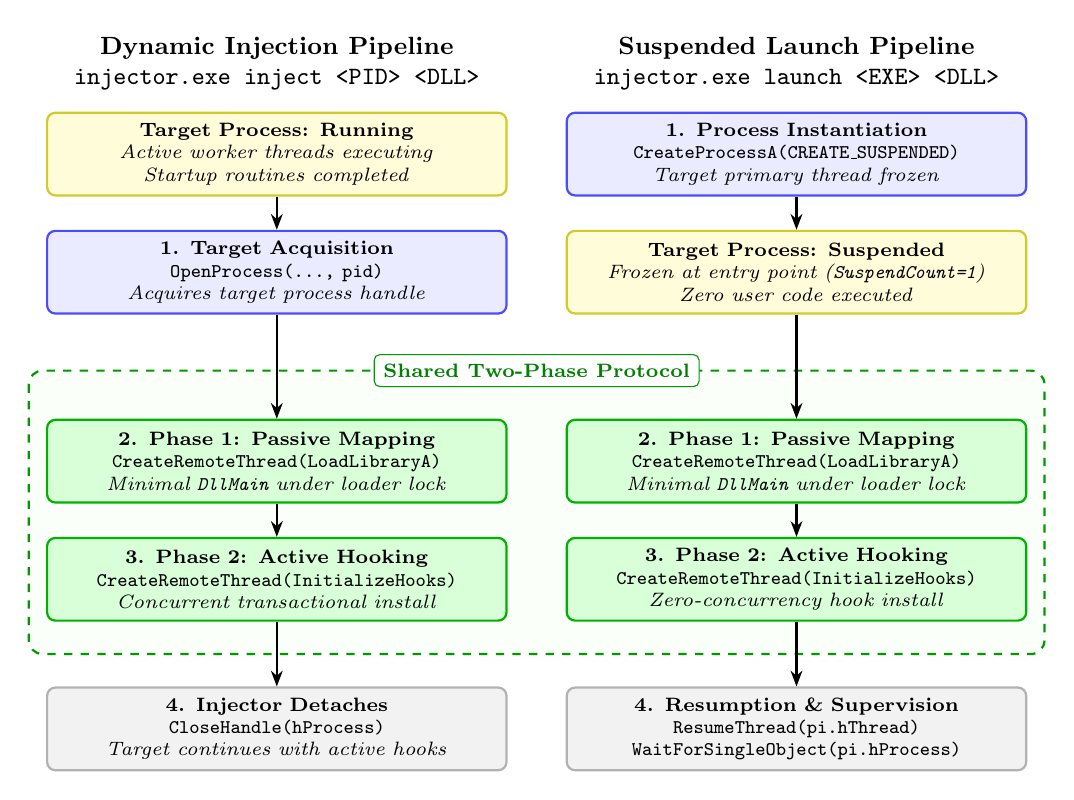
\begin{tikzpicture}[
		>=Stealth,
		font=\scriptsize,
		box/.style={draw, rounded corners=3pt, align=center, thick, text width=5.6cm, minimum height=1.05cm},
		stepnode/.style={box, fill=blue!8, draw=blue!70},
		targetnode/.style={box, fill=yellow!15, draw=yellow!80!black},
		corenode/.style={box, fill=green!15, draw=green!70!black},
		endnode/.style={box, fill=gray!10, draw=gray!60},
		arrow/.style={-{Stealth[length=2.0mm]}, thick}
	]
		% Column Headers
		\node[font=\small\bfseries, align=center] at (0, 1.15) {Dynamic Injection Pipeline\\\texttt{injector.exe inject <PID> <DLL>}};
		\node[font=\small\bfseries, align=center] at (6.6, 1.15) {Suspended Launch Pipeline\\\texttt{injector.exe launch <EXE> <DLL>}};

		% Shared Two-Phase Bracket (Drawn in background)
		\draw[dashed, thick, green!60!black, fill=green!2, rounded corners=5pt] (-3.15, -2.75) rectangle (9.75, -6.35);
		\node[fill=white, draw=green!60!black, font=\scriptsize\bfseries, rounded corners=2pt, text=green!50!black] at (3.3, -2.75) {Shared Two-Phase Protocol};

		% Row 1 (Y = 0.0)
		\node[targetnode] (d_state) at (0, 0) {
			\textbf{Target Process: Running}\\
			\textit{Active worker threads executing}\\
			\textit{Startup routines completed}
		};
		\node[stepnode] (l_create) at (6.6, 0) {
			\textbf{1. Process Instantiation}\\
			\texttt{CreateProcessA(CREATE\_SUSPENDED)}\\
			\textit{Target primary thread frozen}
		};

		% Row 2 (Y = -1.5)
		\node[stepnode] (d_open) at (0, -1.5) {
			\textbf{1. Target Acquisition}\\
			\texttt{OpenProcess(..., pid)}\\
			\textit{Acquires target process handle}
		};
		\node[targetnode] (l_state) at (6.6, -1.5) {
			\textbf{Target Process: Suspended}\\
			\textit{Frozen at entry point (\texttt{SuspendCount=1})}\\
			\textit{Zero user code executed}
		};

		% Row 3 (Y = -3.9)
		\node[corenode] (d_phase1) at (0, -3.9) {
			\textbf{2. Phase 1: Passive Mapping}\\
			\texttt{CreateRemoteThread(LoadLibraryA)}\\
			\textit{Minimal \texttt{DllMain} under loader lock}
		};
		\node[corenode] (l_phase1) at (6.6, -3.9) {
			\textbf{2. Phase 1: Passive Mapping}\\
			\texttt{CreateRemoteThread(LoadLibraryA)}\\
			\textit{Minimal \texttt{DllMain} under loader lock}
		};

		% Row 4 (Y = -5.4)
		\node[corenode] (d_phase2) at (0, -5.4) {
			\textbf{3. Phase 2: Active Hooking}\\
			\texttt{CreateRemoteThread(InitializeHooks)}\\
			\textit{Concurrent transactional install}
		};
		\node[corenode] (l_phase2) at (6.6, -5.4) {
			\textbf{3. Phase 2: Active Hooking}\\
			\texttt{CreateRemoteThread(InitializeHooks)}\\
			\textit{Zero-concurrency hook install}
		};

		% Row 5 (Y = -7.3)
		\node[endnode] (d_end) at (0, -7.3) {
			\textbf{4. Injector Detaches}\\
			\texttt{CloseHandle(hProcess)}\\
			\textit{Target continues with active hooks}
		};
		\node[endnode] (l_end) at (6.6, -7.3) {
			\textbf{4. Resumption \& Supervision}\\
			\texttt{ResumeThread(pi.hThread)}\\
			\texttt{WaitForSingleObject(pi.hProcess)}
		};

		% Vertical Arrows
		\draw[arrow] (d_state) -- (d_open);
		\draw[arrow] (d_open) -- (d_phase1);
		\draw[arrow] (d_phase1) -- (d_phase2);
		\draw[arrow] (d_phase2) -- (d_end);

		\draw[arrow] (l_create) -- (l_state);
		\draw[arrow] (l_state) -- (l_phase1);
		\draw[arrow] (l_phase1) -- (l_phase2);
		\draw[arrow] (l_phase2) -- (l_end);

	\end{tikzpicture}
	\caption{Architectural comparison between Dynamic Injection mode and Suspended Launch mode}
	\label{fig:injection_pipeline_comparison}
\end{figure}


\subsection{DLL Ejection}
\label{subsec:ejection}

When binary instrumentation is no longer required, the payload must detach cleanly so that the target process can continue running without interruption.
As analyzed in \cref{subsec:ejection_sync}, reversing prologue bytes is necessary but not sufficient: in a multi-threaded application, worker threads may already be executing within hook routines when detachment begins.
If the host unmaps the \ac{DLL} via \texttt{FreeLibrary} while a worker thread's instruction pointer points to unmapped memory, the process crashes immediately with an Access Violation.

To prevent this, HookDesigner uses a thread-tracking mechanism during hook detachment.

\subsubsection{Hook Active Thread Tracking}
\label{subsubsec:active_def}

In generated hook functions, thread execution scope is tracked using a RAII helper \texttt{HookActiveThreads}, defined in \texttt{\_user\_logic\_helpers.cpp} and shown in \cref{lst:hook_active_threads_impl}, similar to the one introduced in \cref{subsec:ejection_sync}.

\begin{lstlisting}[language=C++, caption={HookDesigner implementation of active thread tracking in \texttt{\_user\_logic\_helpers.cpp}.}, label={lst:hook_active_threads_impl}, basicstyle=\ttfamily\footnotesize, breaklines=true]
static std::atomic<int> activeThreads{0};

// RAII helper to track active hook execution count
struct HookActiveThreads {
    bool active;
    HookActiveThreads() : active(true) { 
        activeThreads++; 
    }
    ~HookActiveThreads() { 
        if (active) activeThreads--; 
    }
    void Release() {
        if (active) {
            activeThreads--;
            active = false;
        }
    }
};
\end{lstlisting}

\begin{itemize}
	\item \textbf{Lock-Free Counter:} The counter \texttt{activeThreads} is a global atomic variable (\texttt{std::atomic<int>}).
	Its constructor uses atomic increment (\texttt{activeThreads++}) on entry, and its destructor executes atomic decrement (\texttt{activeThreads--}) on exit.
	\item \textbf{Explicit Guard Release for Terminating APIs:}
	As detailed in \cref{subsec:noreturn_adaptation}, functions like \texttt{ExitProcess} or \texttt{RaiseException} never return, so stack unwinding and local destructors are bypassed.
	For this reason I have added the explicit Guard Release method, that the hook explicitly calls \texttt{hook\_active\_threads.Release()} immediately before invoking the terminal trampoline, ensuring the atomic counter decrements before the thread terminates.
\end{itemize}

\subsubsection{The DLL Ejection Mechanism}

When \texttt{injector.exe eject <PID> <DLL>} is executed, it remotely invokes the exported function \texttt{DeinitializeHooks()} via \texttt{CallRemoteExport}, using the same method of the injection, (\cref{lst:rva_offset_invariance}), for preventing Loader Lock deadlock (\cref{subsec:lock_issue}) possible also during ejection.
The payload then performs a five-step ejection sequence, illustrated in \cref{fig:ejection_sequence}:

\begin{figure}[H]
	\centering
	\resizebox{0.98\linewidth}{!}{%
	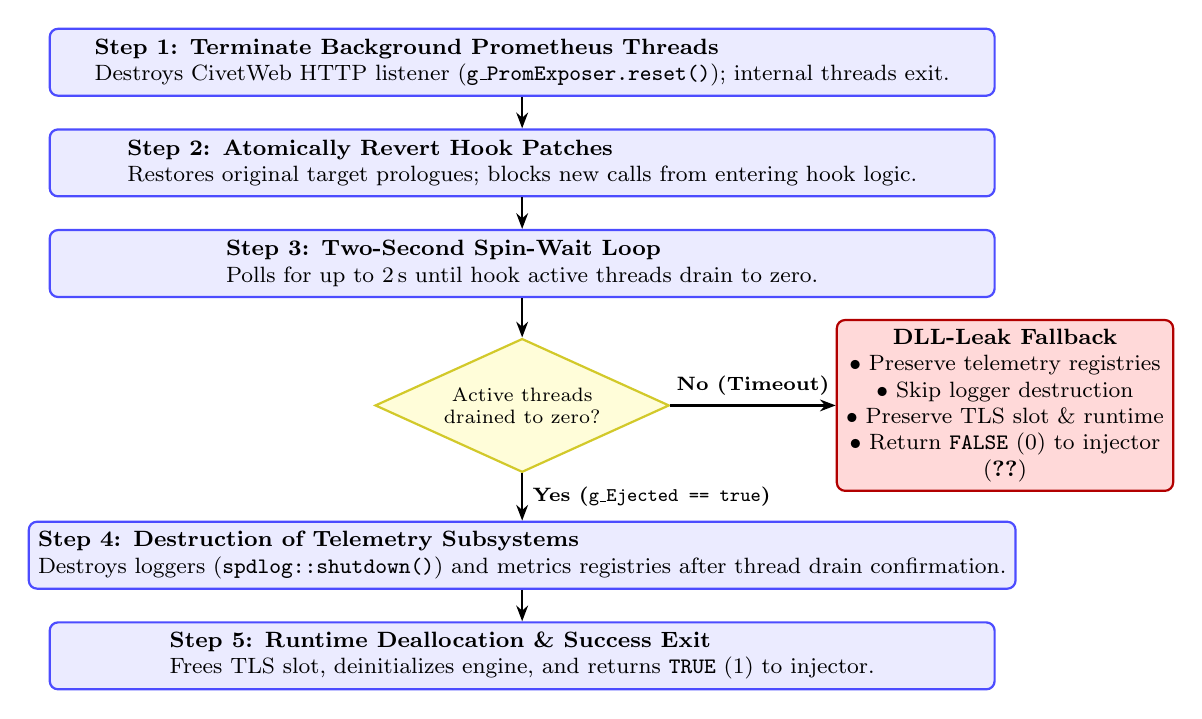
\begin{tikzpicture}[
		>=Stealth,
		font=\footnotesize,
		stepnode/.style={draw, rounded corners=3pt, align=left, thick, fill=blue!8, draw=blue!70, minimum width=12.0cm, minimum height=0.85cm},
		decision/.style={draw, diamond, aspect=2.2, align=center, thick, fill=yellow!15, draw=yellow!80!black, font=\scriptsize},
		term/.style={draw, rounded corners=3pt, align=center, thick, minimum width=3.8cm, minimum height=0.7cm},
		arrow/.style={-{Stealth[length=2.0mm]}, thick}
	]
		\node[stepnode] (s1) at (0, 0) {
			\textbf{Step 1: Terminate Background Prometheus Threads}\\
			Destroys CivetWeb HTTP listener (\texttt{g\_PromExposer.reset()}); internal threads exit.
		};

		\node[stepnode, below=0.4cm of s1] (s2) {
			\textbf{Step 2: Atomically Revert Hook Patches}\\
			Restores original target prologues; blocks new calls from entering hook logic.
		};

		\node[stepnode, below=0.4cm of s2] (s3) {
			\textbf{Step 3: Two-Second Spin-Wait Loop}\\
			Polls for up to 2\,s until hook active threads drain to zero.
		};

		\node[decision, below=0.5cm of s3] (dec) {Active threads\\drained to zero?};

		% Success Branch
		\node[stepnode, below=0.6cm of dec] (s4) {
			\textbf{Step 4: Destruction of Telemetry Subsystems}\\
			Destroys loggers (\texttt{spdlog::shutdown()}) and metrics registries after thread drain confirmation.
		};

		\node[stepnode, below=0.4cm of s4] (s5) {
			\textbf{Step 5: Runtime Deallocation \& Success Exit}\\
			Frees TLS slot, deinitializes engine, and returns \texttt{TRUE} (1) to injector.
		};

		% Failure Branch
		\node[term, fill=red!15, draw=red!70!black, right=2.1cm of dec] (fail) {
			\textbf{DLL-Leak Fallback}\\
			$\bullet$ Preserve telemetry registries\\
			$\bullet$ Skip logger destruction\\
			$\bullet$ Preserve TLS slot \& runtime\\
			$\bullet$ Return \texttt{FALSE} (0) to injector\\
			(\cref{subsec:dll_leak})
		};

		\draw[arrow] (s1) -- (s2);
		\draw[arrow] (s2) -- (s3);
		\draw[arrow] (s3) -- (dec);
		\draw[arrow] (dec) -- node[right, font=\scriptsize\bfseries] {Yes (\texttt{g\_Ejected == true})} (s4);
		\draw[arrow] (s4) -- (s5);
		\draw[arrow] (dec) -- node[above, font=\scriptsize\bfseries] {No (Timeout)} (fail);

	\end{tikzpicture}%
	}
	\caption{Five-step ejection sequence inside \texttt{DeinitializeHooks()}}
	\label{fig:ejection_sequence}
\end{figure}

\begin{enumerate}
	\item \textbf{Terminate Background Listener Threads:}
	The payload resets the Prometheus HTTP exposer.
	The underlying CivetWeb server runs internal threads blocked in \texttt{select()} or \texttt{accept()} calls; destroying the exposer closes the listening socket and terminates these web worker threads cleanly.
	This step must occur first so that external HTTP scraping requests do not arrive while metric families and registries are being destroyed.

	\item \textbf{Atomically Revert Hook Patches:}
	The payload detaches all inline hooks using the engine's transactional API, detailed in \cref{subsec:transactional_patching}
	Once the transaction commits, original prologue bytes are restored in memory.
	New function calls execute the unhooked target code directly; no new threads can enter the hook functions.

	\item \textbf{Two-Second Spin-Wait Loop:}
	Although new calls cannot enter, worker threads that were already inside the hook routines before Step~2 may still be executing.
	To synchronize safely, the payload enters a spin-wait loop with a 2-second (2000\,ms) timeout.
	Under Microsoft Detours, the loop polls only the atomic counter:
	\begin{lstlisting}[language=C++, basicstyle=\ttfamily\footnotesize, numbers=none]
DWORD start = GetTickCount();
while (GetTickCount() - start < 2000) {
    if (activeThreads.load() == 0) {
        Sleep(1000); // Confirmation interval
        if (activeThreads.load() == 0) {
            g_Ejected = true;
            break;
        }
    }
    Sleep(50);
}
	\end{lstlisting}
	Under Frida-Gum, the spin-wait loop adapts based on whether non-returning functions are declared in the policy:
	\begin{lstlisting}[language=C++, basicstyle=\ttfamily\footnotesize, numbers=none]
		DWORD start = GetTickCount();
		while (GetTickCount() - start < 2000) {
			{% if has_noreturn %}
			if (gum_interceptor_flush(interceptor) && activeThreads.load() == 0) {
				Sleep(1000); // Confirmation interval
				if (activeThreads.load() == 0) {
					g_Ejected = true;
					break;
				}
			}
			{% else %}
			if (gum_interceptor_flush(interceptor)) {
				g_Ejected = true;
				break;
			}
			{% endif %}
			Sleep(50);
		}
	\end{lstlisting}
	If the policy intercepts exclusively returning functions, calling \texttt{gum\_}\allowbreak\texttt{interceptor\_}\allowbreak\texttt{flush()} is reliable to confirm that active threads have exited, allowing immediate ejection.
	However, if non-returning functions are present (\texttt{has\_noreturn}), they bypass Frida-Gum's built-in thread tracking.
	In this case, the template emits a dual check requiring both \texttt{gum\_interceptor\_}\allowbreak\texttt{flush()} and \texttt{activeThreads.load() == 0}
	The confirmation interval (\texttt{Sleep(1000\,ms)}) is required because the \texttt{HookActiveThreads} RAII guard decrements the counter inside its destructor, just before the function function returns.
	Consequently, a thread may reach zero while still executing trailing function epilogue instructions (such as register restoration and the final \texttt{ret}) inside the \ac{DLL}'s virtual address space.
	If ejection and module unmapping occurred immediately upon reaching zero, a preempted thread executing these trailing instructions would crash with an Access Violation on unmapped memory.

	\item \textbf{Destruction of Telemetry Subsystems:}
	Only after Step~3 confirms that all worker threads have drained (\texttt{g\_Ejected == true}) the payload destroy the logging and metrics registries.
	This ordering is critical: if loggers or registries were destroyed while a worker thread was still inside \texttt{\_telemetry\_body.cpp} formatting a log or incrementing a counter, the thread would encounter destroyed pointers, triggering a use-after-free crash.

	\item \textbf{Runtime and Resource Deallocation:}
	The payload releases the TLS slot.
	Under Frida-Gum, it unreferences the interceptor and shuts down embedded Frida runtime engine.
	Finally, \texttt{DeinitializeHooks()} returns the outcome to the injector.
\end{enumerate}

\subsubsection{Ejection-Failure DLL Leak Strategy}
\label{subsec:dll_leak}

Despite all the safety measures adopted in the ejection protocol, a persistent challenge in binary instrumentation is the problem of \emph{blocked worker threads}.

\paragraph{The Problem of Hooking Blocking Functions}

In industrial and network-connected applications, worker threads frequently execute blocking system calls, such as:
\begin{itemize}
	\item \texttt{recv()} or \texttt{select()} waiting for incoming network packets on industrial buses;
	\item \texttt{WaitForSingleObject()} or \texttt{Sleep()} waiting for timer ticks or state updates;
	\item \texttt{GetMessage()} or \texttt{ReadFile()} waiting for user input or file I/O completion.
\end{itemize}

If an instrumentation hook intercepts a function that performs a blocking call, a worker thread may enter the hook function, call the original function via the trampoline, and remain blocked in the kernel for seconds, minutes, or hours.
When the user initiates module ejection, Step~2 of \texttt{DeinitializeHooks()} (\cref{fig:ejection_sequence}) successfully restores the original prologue bytes.
However, the blocked thread's activation frame remains frozen on its stack: its return address points directly into \texttt{Hooked<F>} inside the hook \ac{DLL}.

If the injector unloads the \ac{DLL} via \texttt{FreeLibrary}, the operating system unmaps the \ac{DLL}'s code pages from the process's virtual address space.
When the blocking call eventually returns, the worker thread attempts to resume execution at an address that is no longer mapped, triggering an unhandled Access Violation that crashes the host application.

\paragraph{The Controlled Leak Defense Mechanism}

To prevent this event, HookDesigner implements a defense coordinated between the injected \ac{DLL} and the injector utility, illustrated in \cref{fig:leak_strategy_decision_tree}:

\begin{figure}[H]
	\centering
	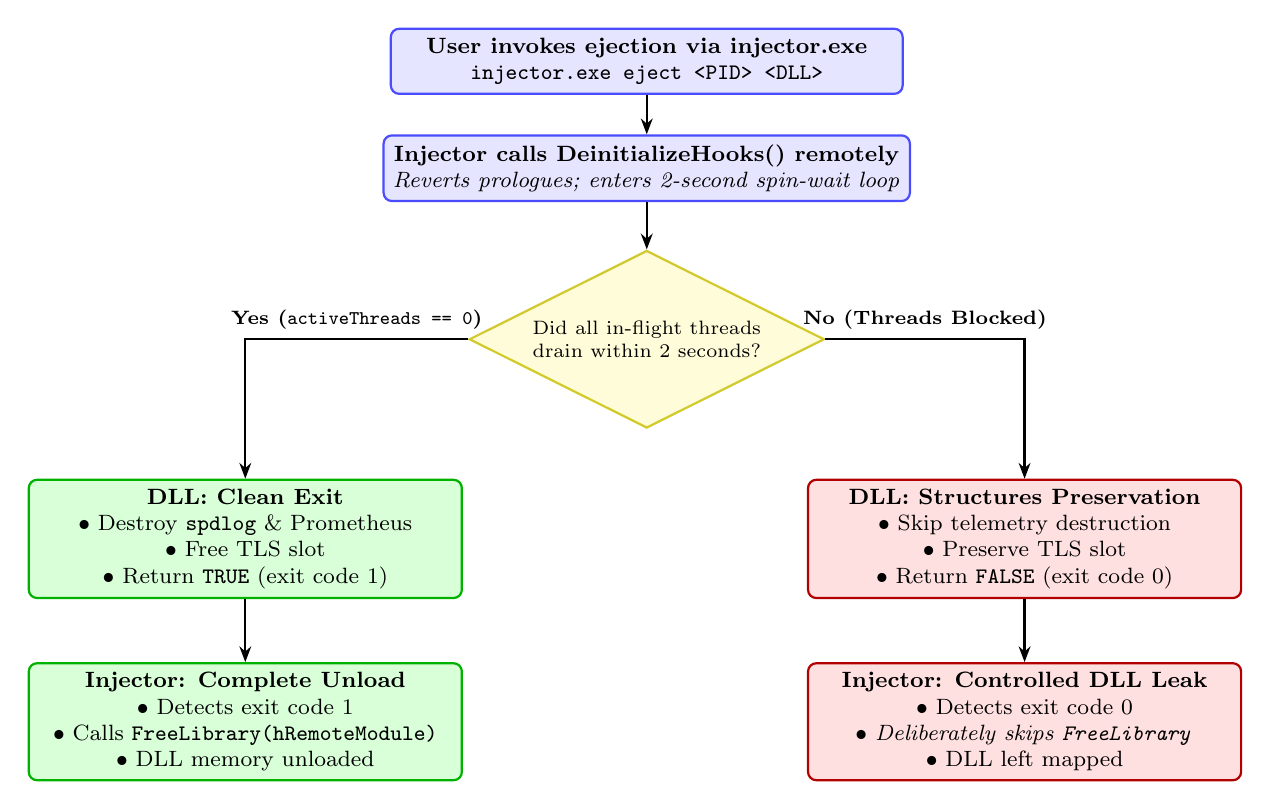
\begin{tikzpicture}[
		>=Stealth,
		font=\footnotesize,
		base/.style={draw, rounded corners=3pt, align=center, thick},
		block/.style={base, fill=blue!10, draw=blue!70, minimum width=6.5cm, minimum height=0.8cm},
		decision/.style={draw, diamond, aspect=2.0, align=center, thick, fill=yellow!15, draw=yellow!80!black, font=\scriptsize},
		success/.style={base, fill=green!15, draw=green!70!black, minimum width=5.5cm, minimum height=1.0cm},
		failure/.style={base, fill=red!12, draw=red!70!black, minimum width=5.5cm, minimum height=1.0cm},
		arrow/.style={-{Stealth[length=2.0mm]}, thick}
	]
		\node[block] (eject_cmd) {\textbf{User invokes ejection via injector.exe}\\\texttt{injector.exe eject <PID> <DLL>}};
		\node[block, below=0.5cm of eject_cmd] (call_deinit) {\textbf{Injector calls DeinitializeHooks() remotely}\\\textit{Reverts prologues; enters 2-second spin-wait loop}};
		\node[decision, below=0.6cm of call_deinit] (check_drain) {Did all in-flight threads\\drain within 2 seconds?};

		% SUCCESS PATH (LEFT)
		\node[success, below left=1.2cm and 1.2cm of check_drain] (succ_dll) {
			\textbf{DLL: Clean Exit}\\
			$\bullet$ Destroy \texttt{spdlog} \& Prometheus\\
			$\bullet$ Free TLS slot\\
			$\bullet$ Return \texttt{TRUE} (exit code 1)
		};
		\node[success, below=0.8cm of succ_dll] (succ_inj) {
			\textbf{Injector: Complete Unload}\\
			$\bullet$ Detects exit code 1\\
			$\bullet$ Calls \texttt{FreeLibrary(hRemoteModule)}\\
			$\bullet$ DLL memory unloaded
		};

		% FAILURE PATH (RIGHT)
		\node[failure, below right=1.2cm and 0.9cm of check_drain] (fail_dll) {
			\textbf{DLL: Structures Preservation}\\
			$\bullet$ Skip telemetry destruction\\
			$\bullet$ Preserve TLS slot\\
			$\bullet$ Return \texttt{FALSE} (exit code 0)
		};
		\node[failure, below=0.8cm of fail_dll] (fail_inj) {
			\textbf{Injector: Controlled DLL Leak}\\
			$\bullet$ Detects exit code 0\\
			$\bullet$ \emph{Deliberately skips \texttt{FreeLibrary}}\\
			$\bullet$ DLL left mapped
		};

		\draw[arrow] (eject_cmd) -- (call_deinit);
		\draw[arrow] (call_deinit) -- (check_drain);
		\draw[arrow] (check_drain) -| node[above, font=\scriptsize\bfseries, pos=0.25] {Yes (\texttt{activeThreads == 0})} (succ_dll);
		\draw[arrow] (succ_dll) -- (succ_inj);
		\draw[arrow] (check_drain) -| node[above, font=\scriptsize\bfseries, pos=0.25] {No (Threads Blocked)} (fail_dll);
		\draw[arrow] (fail_dll) -- (fail_inj);

	\end{tikzpicture}
	\caption{The Ejection-Failure \ac{DLL} Leak Strategy}
	\label{fig:leak_strategy_decision_tree}
\end{figure}

\begin{enumerate}
	\item \textbf{DLL -- Data Structures Preservation (\texttt{DeinitializeHooks}):}
	When the 2-second spin-wait loop expires and threads remain trapped \texttt{DeinitializeHooks()} recognizes that clean ejection is impossible.
	Instead of proceeding with standard cleanup, it:
	\begin{itemize}
		\item \textbf{Preserves Telemetry Registries:} It deliberately skips telemetry data destruction.
		Leaving these structures intact ensures that when the blocked worker thread eventually wakes up and executes post-trampoline telemetry logic, it will not crash due to null pointer dereferences.
		\item \textbf{Preserves TLS Index:} It deliberately skips releasing the allocated TLS slot: when a blocked worker thread unblocks and returns from the target API, it re-enters the hook function's post-logic, calling \texttt{hook\_recursion\_guard.Acquire()} and subsequently \texttt{Release()} inside its RAII destructor (\cref{subsec:recursion_guard}).
		Both routines call \texttt{TlsSetValue} using \texttt{g\_TlsIndex}, if \texttt{TlsFree} had been invoked, \texttt{g\_TlsIndex} would become invalid.
		Preserving \texttt{g\_TlsIndex} guarantees that post-execution re-entrancy tracking and RAII destructors complete safely without process corruption.
		\item \textbf{Returns Failure Code:} It returns \texttt{FALSE} (\texttt{0}) to the injector.
	\end{itemize}

	\item \textbf{Injector -- Safety Fallback:}
	The injector inspects the remote thread's exit code, as shown in \cref{lst:injector_eject_fallback}:
	\begin{lstlisting}[language=C++, caption={Injector fallback logic}, label={lst:injector_eject_fallback}, basicstyle=\ttfamily\footnotesize, breaklines=true]
DWORD deinitExitCode = 1; // Default to success (TRUE)

CallRemoteExport(hProcess, hRemoteModule, dllPath, "DeinitializeHooks", &deinitExitCode);

if (deinitExitCode == 0) { // FALSE: DLL leak fallback
    std::cout << "[WARNING] Skipping FreeLibrary (leaking DLL in target memory)";

} else { // TRUE: Clean drain
    HANDLE hThread = CreateRemoteThread(hProcess, NULL, 0, 
        (LPTHREAD_START_ROUTINE)pFreeLibrary, (LPVOID)hRemoteModule, 0, NULL);
    
    WaitForSingleObject(hThread, INFINITE);
    
    CloseHandle(hThread);
}
	\end{lstlisting}
	If \texttt{deinitExitCode} is \texttt{0}, \texttt{injector.exe} outputs a warning and \emph{deliberately skips} calling \texttt{FreeLibrary}.
	The hook \ac{DLL} remains mapped in the target process's virtual memory space.
\end{enumerate}


From a software engineering perspective, leaking memory is typically considered a defect.
However, in binary instrumentation—particularly in critical industrial software—leaking a \ac{DLL} under ejection failure is a safety-oriented design decision.

Considering the two alternatives when ejection encounters blocked threads:
\begin{enumerate}
	\item \textbf{Strict Memory Reclamation (\texttt{FreeLibrary}):} The injector unmaps the module.
	When the blocked thread wakes up, its return address points to deallocated memory (\texttt{MEM\_FREE}), triggering an instantaneous Access Violation, that makes crash the host process.
	\item \textbf{Controlled Payload Leak (HookDesigner Fallback):} The module remains mapped in virtual memory.
	Because hooks were already reverted in Step~2, no \emph{new} calls can ever enter the \ac{DLL}.
	The memory overhead of the leaked payload is negligible (typically under 1\,MB).
	When the blocked thread eventually unblocks, it unwinds its stack through the still-valid code pages, returns to the host application, the ejection mechanism can be repeated and the DLL can be freed.
\end{enumerate}

In critical environments, often \emph{process stability supersedes complete memory reclamation}.
By combining atomic prologue reversion with the controlled \ac{DLL} leak fallback, HookDesigner guarantees that instrumentation can be safely detached at runtime without risking process termination.




\include{results}

\include{conclusion}

% Bibliography using biber; comment this and uncomment the following lines to use bibtex instead
\nocite{*}
\printbibliography
% \bibliographystyle{alphaurl}
% \bibliography{bib}

\end{document}

